\documentclass[twoside]{book}

% Packages required by doxygen
\usepackage{calc}
\usepackage{doxygen}
\usepackage{graphicx}
\usepackage[utf8]{inputenc}
\usepackage{makeidx}
\usepackage{multicol}
\usepackage{multirow}
\usepackage{fixltx2e}
\PassOptionsToPackage{warn}{textcomp}
\usepackage{textcomp}
\usepackage[nointegrals]{wasysym}
\usepackage[table]{xcolor}

% Font selection
\usepackage[T1]{fontenc}
\usepackage{mathptmx}
\usepackage[scaled=.90]{helvet}
\usepackage{courier}
\usepackage{amssymb}
\usepackage{sectsty}
\renewcommand{\familydefault}{\sfdefault}
\allsectionsfont{%
  \fontseries{bc}\selectfont%
  \color{darkgray}%
}
\renewcommand{\DoxyLabelFont}{%
  \fontseries{bc}\selectfont%
  \color{darkgray}%
}
\newcommand{\+}{\discretionary{\mbox{\scriptsize$\hookleftarrow$}}{}{}}

% Page & text layout
\usepackage{geometry}
\geometry{%
  a4paper,%
  top=2.5cm,%
  bottom=2.5cm,%
  left=2.5cm,%
  right=2.5cm%
}
\tolerance=750
\hfuzz=15pt
\hbadness=750
\setlength{\emergencystretch}{15pt}
\setlength{\parindent}{0cm}
\setlength{\parskip}{0.2cm}
\makeatletter
\renewcommand{\paragraph}{%
  \@startsection{paragraph}{4}{0ex}{-1.0ex}{1.0ex}{%
    \normalfont\normalsize\bfseries\SS@parafont%
  }%
}
\renewcommand{\subparagraph}{%
  \@startsection{subparagraph}{5}{0ex}{-1.0ex}{1.0ex}{%
    \normalfont\normalsize\bfseries\SS@subparafont%
  }%
}
\makeatother

% Headers & footers
\usepackage{fancyhdr}
\pagestyle{fancyplain}
\fancyhead[LE]{\fancyplain{}{\bfseries\thepage}}
\fancyhead[CE]{\fancyplain{}{}}
\fancyhead[RE]{\fancyplain{}{\bfseries\leftmark}}
\fancyhead[LO]{\fancyplain{}{\bfseries\rightmark}}
\fancyhead[CO]{\fancyplain{}{}}
\fancyhead[RO]{\fancyplain{}{\bfseries\thepage}}
\fancyfoot[LE]{\fancyplain{}{}}
\fancyfoot[CE]{\fancyplain{}{}}
\fancyfoot[RE]{\fancyplain{}{\bfseries\scriptsize Generated on Mon Sep 22 2014 14\+:12\+:35 for Phd\+Thesis by Doxygen }}
\fancyfoot[LO]{\fancyplain{}{\bfseries\scriptsize Generated on Mon Sep 22 2014 14\+:12\+:35 for Phd\+Thesis by Doxygen }}
\fancyfoot[CO]{\fancyplain{}{}}
\fancyfoot[RO]{\fancyplain{}{}}
\renewcommand{\footrulewidth}{0.4pt}
\renewcommand{\chaptermark}[1]{%
  \markboth{#1}{}%
}
\renewcommand{\sectionmark}[1]{%
  \markright{\thesection\ #1}%
}

% Indices & bibliography
\usepackage{natbib}
\usepackage[titles]{tocloft}
\setcounter{tocdepth}{3}
\setcounter{secnumdepth}{5}
\makeindex

% Hyperlinks (required, but should be loaded last)
\usepackage{ifpdf}
\ifpdf
  \usepackage[pdftex,pagebackref=true]{hyperref}
\else
  \usepackage[ps2pdf,pagebackref=true]{hyperref}
\fi
\hypersetup{%
  colorlinks=true,%
  linkcolor=blue,%
  citecolor=blue,%
  unicode%
}

% Custom commands
\newcommand{\clearemptydoublepage}{%
  \newpage{\pagestyle{empty}\cleardoublepage}%
}


%===== C O N T E N T S =====

\begin{document}

% Titlepage & ToC
\hypersetup{pageanchor=false,
             bookmarks=true,
             bookmarksnumbered=true,
             pdfencoding=unicode
            }
\pagenumbering{roman}
\begin{titlepage}
\vspace*{7cm}
\begin{center}%
{\Large Phd\+Thesis }\\
\vspace*{1cm}
{\large Generated by Doxygen 1.8.7}\\
\vspace*{0.5cm}
{\small Mon Sep 22 2014 14:12:35}\\
\end{center}
\end{titlepage}
\clearemptydoublepage
\tableofcontents
\clearemptydoublepage
\pagenumbering{arabic}
\hypersetup{pageanchor=true}

%--- Begin generated contents ---
\chapter{Hierarchical Index}
\section{Class Hierarchy}
This inheritance list is sorted roughly, but not completely, alphabetically\+:\begin{DoxyCompactList}
\item \contentsline{section}{\+\_\+label}{\pageref{struct__label}}{}
\item \contentsline{section}{Complex\+Network\+Constructor}{\pageref{class_complex_network_constructor}}{}
\item \contentsline{section}{Complex\+Network\+To\+Matlab}{\pageref{class_complex_network_to_matlab}}{}
\item \contentsline{section}{Complex\+Network\+V2$<$ N, E $>$}{\pageref{class_complex_network_v2}}{}
\item \contentsline{section}{Co\+Ocurrence\+Equation}{\pageref{class_co_ocurrence_equation}}{}
\begin{DoxyCompactList}
\item \contentsline{section}{Add\+One\+Co\+Ocurrence\+Equation}{\pageref{class_add_one_co_ocurrence_equation}}{}
\item \contentsline{section}{Reinforcement\+Co\+Ocurrence\+Equation}{\pageref{class_reinforcement_co_ocurrence_equation}}{}
\end{DoxyCompactList}
\item \contentsline{section}{Database\+Reader}{\pageref{class_database_reader}}{}
\begin{DoxyCompactList}
\item \contentsline{section}{K\+Fold\+Database\+Reader\+:\+:Path\+Database\+Reader}{\pageref{class_k_fold_database_reader_1_1_path_database_reader}}{}
\item \contentsline{section}{Sun\+Database\+Reader}{\pageref{class_sun_database_reader}}{}
\end{DoxyCompactList}
\item \contentsline{section}{Complex\+Network\+V2$<$ N, E $>$\+:\+:Edge\+Iterator}{\pageref{class_complex_network_v2_1_1_edge_iterator}}{}
\item \contentsline{section}{Feature\+Abstract}{\pageref{class_feature_abstract}}{}
\begin{DoxyCompactList}
\item \contentsline{section}{Feature$<$ T $>$}{\pageref{class_feature}}{}
\item \contentsline{section}{Feature$<$ float $>$}{\pageref{class_feature}}{}
\begin{DoxyCompactList}
\item \contentsline{section}{Area\+Feature}{\pageref{class_area_feature}}{}
\end{DoxyCompactList}
\item \contentsline{section}{Feature$<$ label $>$}{\pageref{class_feature}}{}
\begin{DoxyCompactList}
\item \contentsline{section}{Label\+Feature}{\pageref{class_label_feature}}{}
\end{DoxyCompactList}
\item \contentsline{section}{Feature$<$ unsigned int $>$}{\pageref{class_feature}}{}
\begin{DoxyCompactList}
\item \contentsline{section}{Orientation\+Feature}{\pageref{class_orientation_feature}}{}
\end{DoxyCompactList}
\end{DoxyCompactList}
\item \contentsline{section}{Feature\+Abstract\+Key}{\pageref{class_feature_abstract_key}}{}
\item \contentsline{section}{Feature\+Abstract\+Ptr}{\pageref{class_feature_abstract_ptr}}{}
\item \contentsline{section}{Feature\+Factory\+Abstract}{\pageref{class_feature_factory_abstract}}{}
\begin{DoxyCompactList}
\item \contentsline{section}{Area\+Feature\+Factory}{\pageref{class_area_feature_factory}}{}
\item \contentsline{section}{Label\+Feature\+Factory}{\pageref{class_label_feature_factory}}{}
\item \contentsline{section}{Orientation\+Feature\+Factory}{\pageref{class_orientation_feature_factory}}{}
\end{DoxyCompactList}
\item \contentsline{section}{get\+Weight}{\pageref{classget_weight}}{}
\item \contentsline{section}{Graph\+Utilities}{\pageref{class_graph_utilities}}{}
\item \contentsline{section}{Features\+Complex\+Network\+:\+:header}{\pageref{struct_features_complex_network_1_1header}}{}
\item \contentsline{section}{Iterative\+Random\+Walk}{\pageref{class_iterative_random_walk}}{}
\item \contentsline{section}{K\+Fold\+Database\+Reader}{\pageref{class_k_fold_database_reader}}{}
\item \contentsline{section}{Label\+Guesser}{\pageref{class_label_guesser}}{}
\item \contentsline{section}{Label\+Guesser\+Experiment}{\pageref{class_label_guesser_experiment}}{}
\item \contentsline{section}{Labels\+Validation\+Experiment}{\pageref{class_labels_validation_experiment}}{}
\item \contentsline{section}{Link}{\pageref{class_link}}{}
\item List\+Digraph\begin{DoxyCompactList}
\item \contentsline{section}{Complex\+Network$<$ N, E $>$}{\pageref{class_complex_network}}{}
\item \contentsline{section}{Complex\+Network$<$ Feature\+Abstract\+Ptr, Link $>$}{\pageref{class_complex_network}}{}
\begin{DoxyCompactList}
\item \contentsline{section}{Features\+Complex\+Network}{\pageref{class_features_complex_network}}{}
\end{DoxyCompactList}
\item \contentsline{section}{Complex\+Network$<$ Node\+String, Link $>$}{\pageref{class_complex_network}}{}
\end{DoxyCompactList}
\item \contentsline{section}{node\+\_\+t}{\pageref{classnode__t}}{}
\item \contentsline{section}{Complex\+Network\+V2$<$ N, E $>$\+:\+:Node\+Iterator}{\pageref{class_complex_network_v2_1_1_node_iterator}}{}
\item \contentsline{section}{Features\+Complex\+Network\+:\+:Node\+Reader}{\pageref{class_features_complex_network_1_1_node_reader}}{}
\item \contentsline{section}{Node\+String}{\pageref{class_node_string}}{}
\item Q\+Label\begin{DoxyCompactList}
\item \contentsline{section}{Supervised\+Image\+Viewer\+Widget}{\pageref{class_supervised_image_viewer_widget}}{}
\end{DoxyCompactList}
\item Q\+Main\+Window\begin{DoxyCompactList}
\item \contentsline{section}{Complex\+Network\+Visualizer}{\pageref{class_complex_network_visualizer}}{}
\end{DoxyCompactList}
\item Q\+Widget\begin{DoxyCompactList}
\item \contentsline{section}{Area\+Feature\+Extraction\+Window}{\pageref{class_area_feature_extraction_window}}{}
\item \contentsline{section}{Complex\+Network\+Viewer\+Widget}{\pageref{class_complex_network_viewer_widget}}{}
\item \contentsline{section}{Database\+Visualizer\+Widget}{\pageref{class_database_visualizer_widget}}{}
\item \contentsline{section}{G\+Main\+Window}{\pageref{class_g_main_window}}{}
\end{DoxyCompactList}
\item \contentsline{section}{Random\+Walk\+Test}{\pageref{class_random_walk_test}}{}
\item \contentsline{section}{Random\+Walk\+Test2}{\pageref{class_random_walk_test2}}{}
\item \contentsline{section}{Region}{\pageref{class_region}}{}
\item \contentsline{section}{Segmenter}{\pageref{class_segmenter}}{}
\item Structure\begin{DoxyCompactList}
\item \contentsline{section}{compute\+\_\+modularity.\+Bt}{\pageref{classcompute__modularity_1_1_bt}}{}
\item \contentsline{section}{compute\+\_\+modularity.\+Edge}{\pageref{classcompute__modularity_1_1_edge}}{}
\item \contentsline{section}{compute\+\_\+modularity.\+Header}{\pageref{classcompute__modularity_1_1_header}}{}
\item \contentsline{section}{compute\+\_\+modularity.\+Label\+Node}{\pageref{classcompute__modularity_1_1_label_node}}{}
\item \contentsline{section}{compute\+\_\+modularity.\+Linka}{\pageref{classcompute__modularity_1_1_linka}}{}
\item \contentsline{section}{compute\+\_\+modularity.\+Node}{\pageref{classcompute__modularity_1_1_node}}{}
\end{DoxyCompactList}
\item \contentsline{section}{S\+U\+N\+Random\+Folder\+Generator}{\pageref{class_s_u_n_random_folder_generator}}{}
\item \contentsline{section}{Supervised\+Image}{\pageref{class_supervised_image}}{}
\end{DoxyCompactList}

\chapter{Class Index}
\section{Class List}
Here are the classes, structs, unions and interfaces with brief descriptions\+:\begin{DoxyCompactList}
\item\contentsline{section}{\hyperlink{class_area_feature_extractor}{Area\+Feature\+Extractor} }{\pageref{class_area_feature_extractor}}{}
\item\contentsline{section}{\hyperlink{class_complex_network}{Complex\+Network$<$ N\+O\+D\+E\+\_\+\+T\+Y\+P\+E, E\+D\+G\+E\+\_\+\+T\+Y\+P\+E $>$} \\*Rede Complexa }{\pageref{class_complex_network}}{}
\item\contentsline{section}{\hyperlink{class_complex_network_constructor}{Complex\+Network\+Constructor} }{\pageref{class_complex_network_constructor}}{}
\item\contentsline{section}{\hyperlink{class_database_reader}{Database\+Reader} }{\pageref{class_database_reader}}{}
\item\contentsline{section}{\hyperlink{class_edge}{Edge$<$ N\+O\+D\+E\+\_\+\+T\+Y\+P\+E, E\+D\+G\+E\+\_\+\+T\+Y\+P\+E $>$} }{\pageref{class_edge}}{}
\item\contentsline{section}{\hyperlink{class_feature}{Feature} }{\pageref{class_feature}}{}
\item\contentsline{section}{\hyperlink{class_feature_extractor}{Feature\+Extractor} }{\pageref{class_feature_extractor}}{}
\item\contentsline{section}{\hyperlink{class_link}{Link} }{\pageref{class_link}}{}
\item\contentsline{section}{\hyperlink{class_node}{Node$<$ N\+O\+D\+E\+\_\+\+T\+Y\+P\+E, E\+D\+G\+E\+\_\+\+T\+Y\+P\+E $>$} }{\pageref{class_node}}{}
\item\contentsline{section}{\hyperlink{classnode__t}{node\+\_\+t} }{\pageref{classnode__t}}{}
\item\contentsline{section}{\hyperlink{class_region}{Region} }{\pageref{class_region}}{}
\item\contentsline{section}{\hyperlink{class_sun_database_reader}{Sun\+Database\+Reader} }{\pageref{class_sun_database_reader}}{}
\item\contentsline{section}{\hyperlink{class_supervised_image}{Supervised\+Image} }{\pageref{class_supervised_image}}{}
\end{DoxyCompactList}

\chapter{File Index}
\section{File List}
Here is a list of all files with brief descriptions\+:\begin{DoxyCompactList}
\item\contentsline{section}{src/\hyperlink{_complex_network_8cpp}{Complex\+Network.\+cpp} }{\pageref{_complex_network_8cpp}}{}
\item\contentsline{section}{src/\hyperlink{_complex_network_8hpp}{Complex\+Network.\+hpp} }{\pageref{_complex_network_8hpp}}{}
\item\contentsline{section}{src/\hyperlink{_edge_8cpp}{Edge.\+cpp} }{\pageref{_edge_8cpp}}{}
\item\contentsline{section}{src/\hyperlink{_edge_8hpp}{Edge.\+hpp} }{\pageref{_edge_8hpp}}{}
\item\contentsline{section}{src/\hyperlink{main_8cpp}{main.\+cpp} }{\pageref{main_8cpp}}{}
\item\contentsline{section}{src/\hyperlink{_node_8cpp}{Node.\+cpp} }{\pageref{_node_8cpp}}{}
\item\contentsline{section}{src/\hyperlink{_node_8hpp}{Node.\+hpp} }{\pageref{_node_8hpp}}{}
\end{DoxyCompactList}

\chapter{Class Documentation}
\hypertarget{class_area_feature_extractor}{\section{Area\+Feature\+Extractor Class Reference}
\label{class_area_feature_extractor}\index{Area\+Feature\+Extractor@{Area\+Feature\+Extractor}}
}


{\ttfamily \#include $<$Area\+Feature\+Extractor.\+hpp$>$}

\subsection*{Public Member Functions}
\begin{DoxyCompactItemize}
\item 
\hyperlink{class_area_feature_extractor_ab183d05cccc841a75b368ce55d2f37bb}{Area\+Feature\+Extractor} ()
\item 
Q\+Vector$<$ float $>$ \hyperlink{class_area_feature_extractor_a9dfd50444d94b1fd82fdd6ec0f9163c3}{do\+Extraction} (\hyperlink{class_region}{Region} $\ast$r)
\item 
void \hyperlink{class_area_feature_extractor_a9969af2ec658c4404651cc13bef00089}{do\+Discretization} (Q\+Vector$<$ float $>$ \&feature, int \hyperlink{class_feature_extractor_a1d800b4e5f3af7c758bfc5f157110681}{discretization})
\item 
const char $\ast$ \hyperlink{class_area_feature_extractor_af4d987a1253cadd506280d3c8b99d860}{get\+Feature\+Name} ()
\end{DoxyCompactItemize}
\subsection*{Private Member Functions}
\begin{DoxyCompactItemize}
\item 
void \hyperlink{class_area_feature_extractor_a01c1c501f11f6b986e46b7b1fe2d4508}{discretize} (int quantization)
\end{DoxyCompactItemize}
\subsection*{Additional Inherited Members}


Inheritance diagram for Area\+Feature\+Extractor\+:\nopagebreak
\begin{figure}[H]
\begin{center}
\leavevmode
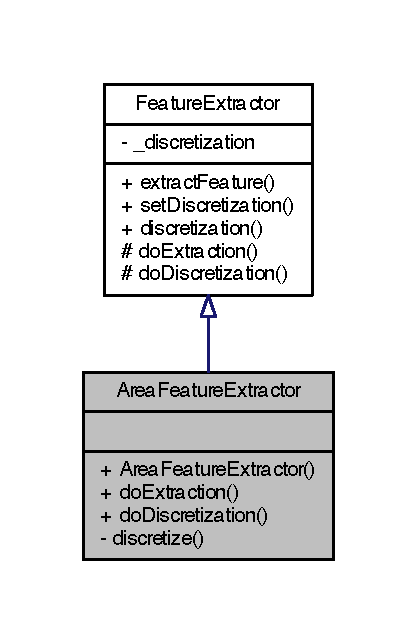
\includegraphics[width=200pt]{class_area_feature_extractor__inherit__graph}
\end{center}
\end{figure}


Collaboration diagram for Area\+Feature\+Extractor\+:\nopagebreak
\begin{figure}[H]
\begin{center}
\leavevmode
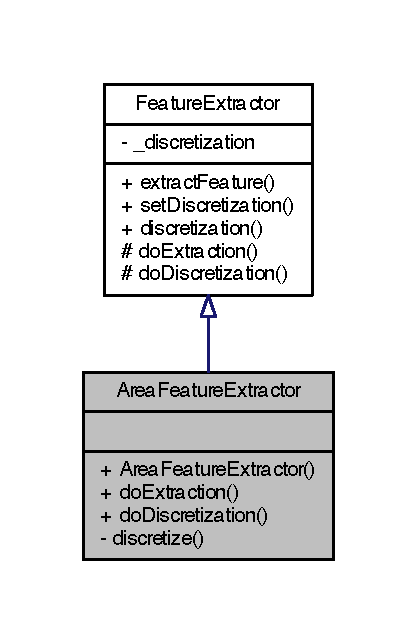
\includegraphics[width=200pt]{class_area_feature_extractor__coll__graph}
\end{center}
\end{figure}


\subsection{Constructor \& Destructor Documentation}
\hypertarget{class_area_feature_extractor_ab183d05cccc841a75b368ce55d2f37bb}{\index{Area\+Feature\+Extractor@{Area\+Feature\+Extractor}!Area\+Feature\+Extractor@{Area\+Feature\+Extractor}}
\index{Area\+Feature\+Extractor@{Area\+Feature\+Extractor}!Area\+Feature\+Extractor@{Area\+Feature\+Extractor}}
\subsubsection[{Area\+Feature\+Extractor}]{\setlength{\rightskip}{0pt plus 5cm}Area\+Feature\+Extractor\+::\+Area\+Feature\+Extractor (
\begin{DoxyParamCaption}
{}
\end{DoxyParamCaption}
)}}\label{class_area_feature_extractor_ab183d05cccc841a75b368ce55d2f37bb}


\subsection{Member Function Documentation}
\hypertarget{class_area_feature_extractor_a01c1c501f11f6b986e46b7b1fe2d4508}{\index{Area\+Feature\+Extractor@{Area\+Feature\+Extractor}!discretize@{discretize}}
\index{discretize@{discretize}!Area\+Feature\+Extractor@{Area\+Feature\+Extractor}}
\subsubsection[{discretize}]{\setlength{\rightskip}{0pt plus 5cm}void Area\+Feature\+Extractor\+::discretize (
\begin{DoxyParamCaption}
\item[{int}]{quantization}
\end{DoxyParamCaption}
)\hspace{0.3cm}{\ttfamily [private]}}}\label{class_area_feature_extractor_a01c1c501f11f6b986e46b7b1fe2d4508}
\hypertarget{class_area_feature_extractor_a9969af2ec658c4404651cc13bef00089}{\index{Area\+Feature\+Extractor@{Area\+Feature\+Extractor}!do\+Discretization@{do\+Discretization}}
\index{do\+Discretization@{do\+Discretization}!Area\+Feature\+Extractor@{Area\+Feature\+Extractor}}
\subsubsection[{do\+Discretization}]{\setlength{\rightskip}{0pt plus 5cm}void Area\+Feature\+Extractor\+::do\+Discretization (
\begin{DoxyParamCaption}
\item[{Q\+Vector$<$ float $>$ \&}]{feature, }
\item[{int}]{discretization}
\end{DoxyParamCaption}
)\hspace{0.3cm}{\ttfamily [virtual]}}}\label{class_area_feature_extractor_a9969af2ec658c4404651cc13bef00089}


Reimplemented from \hyperlink{class_feature_extractor_aa72a103a311a391eafdd0916c8ffabce}{Feature\+Extractor}.



Here is the call graph for this function\+:\nopagebreak
\begin{figure}[H]
\begin{center}
\leavevmode
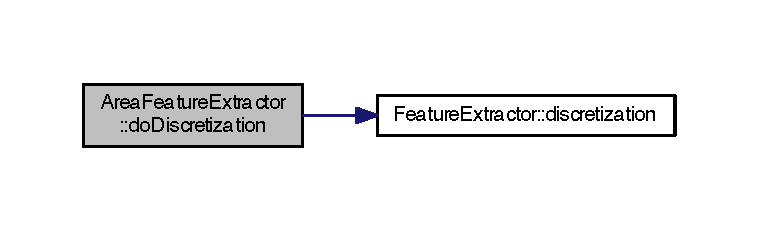
\includegraphics[width=350pt]{class_area_feature_extractor_a9969af2ec658c4404651cc13bef00089_cgraph}
\end{center}
\end{figure}


\hypertarget{class_area_feature_extractor_a9dfd50444d94b1fd82fdd6ec0f9163c3}{\index{Area\+Feature\+Extractor@{Area\+Feature\+Extractor}!do\+Extraction@{do\+Extraction}}
\index{do\+Extraction@{do\+Extraction}!Area\+Feature\+Extractor@{Area\+Feature\+Extractor}}
\subsubsection[{do\+Extraction}]{\setlength{\rightskip}{0pt plus 5cm}Q\+Vector$<$ float $>$ Area\+Feature\+Extractor\+::do\+Extraction (
\begin{DoxyParamCaption}
\item[{{\bf Region} $\ast$}]{r}
\end{DoxyParamCaption}
)\hspace{0.3cm}{\ttfamily [virtual]}}}\label{class_area_feature_extractor_a9dfd50444d94b1fd82fdd6ec0f9163c3}


Reimplemented from \hyperlink{class_feature_extractor_af4afca623abc12c0af3572b2189d0825}{Feature\+Extractor}.



Here is the call graph for this function\+:\nopagebreak
\begin{figure}[H]
\begin{center}
\leavevmode
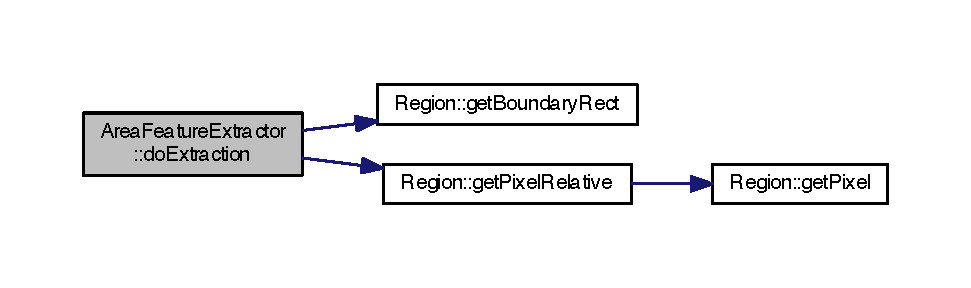
\includegraphics[width=350pt]{class_area_feature_extractor_a9dfd50444d94b1fd82fdd6ec0f9163c3_cgraph}
\end{center}
\end{figure}


\hypertarget{class_area_feature_extractor_af4d987a1253cadd506280d3c8b99d860}{\index{Area\+Feature\+Extractor@{Area\+Feature\+Extractor}!get\+Feature\+Name@{get\+Feature\+Name}}
\index{get\+Feature\+Name@{get\+Feature\+Name}!Area\+Feature\+Extractor@{Area\+Feature\+Extractor}}
\subsubsection[{get\+Feature\+Name}]{\setlength{\rightskip}{0pt plus 5cm}const char $\ast$ Area\+Feature\+Extractor\+::get\+Feature\+Name (
\begin{DoxyParamCaption}
{}
\end{DoxyParamCaption}
)\hspace{0.3cm}{\ttfamily [virtual]}}}\label{class_area_feature_extractor_af4d987a1253cadd506280d3c8b99d860}


Reimplemented from \hyperlink{class_feature_extractor_a12e9b0c683be94146a5c4fbd2d48967f}{Feature\+Extractor}.



The documentation for this class was generated from the following files\+:\begin{DoxyCompactItemize}
\item 
src/\hyperlink{_area_feature_extractor_8hpp}{Area\+Feature\+Extractor.\+hpp}\item 
src/\hyperlink{_area_feature_extractor_8cpp}{Area\+Feature\+Extractor.\+cpp}\end{DoxyCompactItemize}

\hypertarget{class_complex_network}{\section{Complex\+Network$<$ N\+O\+D\+E\+\_\+\+T\+Y\+P\+E, E\+D\+G\+E\+\_\+\+T\+Y\+P\+E $>$ Class Template Reference}
\label{class_complex_network}\index{Complex\+Network$<$ N\+O\+D\+E\+\_\+\+T\+Y\+P\+E, E\+D\+G\+E\+\_\+\+T\+Y\+P\+E $>$@{Complex\+Network$<$ N\+O\+D\+E\+\_\+\+T\+Y\+P\+E, E\+D\+G\+E\+\_\+\+T\+Y\+P\+E $>$}}
}


{\ttfamily \#include $<$Complex\+Network.\+hpp$>$}

\subsection*{Classes}
\begin{DoxyCompactItemize}
\item 
class \hyperlink{class_complex_network_1_1_edge_iterator}{Edge\+Iterator}
\item 
class \hyperlink{class_complex_network_1_1_node_iterator}{Node\+Iterator}
\end{DoxyCompactItemize}
\subsection*{Public Member Functions}
\begin{DoxyCompactItemize}
\item 
\hyperlink{class_complex_network_a4a16e825e1d8b487067ca21d677617a3}{Complex\+Network} (bool \hyperlink{class_complex_network_ae1f8a32f89d84aab42475d8fe46dfa09}{directed}=true)
\item 
virtual \hyperlink{_complex_network_8hpp_a8323334ca788fde39682469321590d52}{node\+\_\+id} \hyperlink{class_complex_network_af2c31ca0d2142dafa1d88ca3ff22356f}{add\+Node} (const N\+O\+D\+E\+\_\+\+T\+Y\+P\+E \&n)
\item 
virtual N\+O\+D\+E\+\_\+\+T\+Y\+P\+E $\ast$ \hyperlink{class_complex_network_a3711aff250a942a9ad61d0571be82c43}{get\+Node} (\hyperlink{_complex_network_8hpp_a8323334ca788fde39682469321590d52}{node\+\_\+id} id)
\item 
virtual bool \hyperlink{class_complex_network_a33f2b4528cc31296ede98be7e6dcd600}{remove\+Node} (\hyperlink{_complex_network_8hpp_a8323334ca788fde39682469321590d52}{node\+\_\+id} id)
\item 
virtual void \hyperlink{class_complex_network_a52c25eb9c9c642a39681e4040fc0a17d}{add\+Edge} (\hyperlink{_complex_network_8hpp_a8323334ca788fde39682469321590d52}{node\+\_\+id} from, \hyperlink{_complex_network_8hpp_a8323334ca788fde39682469321590d52}{node\+\_\+id} to, const E\+D\+G\+E\+\_\+\+T\+Y\+P\+E \&e)
\item 
virtual E\+D\+G\+E\+\_\+\+T\+Y\+P\+E $\ast$ \hyperlink{class_complex_network_a6a1c638e4604efe06c12ce3065020ec1}{get\+Edge} (\hyperlink{_complex_network_8hpp_a8323334ca788fde39682469321590d52}{node\+\_\+id} from, \hyperlink{_complex_network_8hpp_a8323334ca788fde39682469321590d52}{node\+\_\+id} to)
\item 
virtual E\+D\+G\+E\+\_\+\+T\+Y\+P\+E $\ast$ \hyperlink{class_complex_network_ad440008416fc33500754d77b2532560f}{get\+Edge\+From\+Edge\+Id} (\hyperlink{_complex_network_8hpp_ad7d18d7b90a45b6625704e92d10aa3a0}{edge\+\_\+id} id)
\item 
virtual bool \hyperlink{class_complex_network_a9b2c7df561a2ad5fc14b04a5c5c56828}{remove\+Edge} (\hyperlink{_complex_network_8hpp_a8323334ca788fde39682469321590d52}{node\+\_\+id} from, \hyperlink{_complex_network_8hpp_a8323334ca788fde39682469321590d52}{node\+\_\+id} to)
\item 
virtual void \hyperlink{class_complex_network_a64db5949375a84eba3d9ff559d68fc6e}{clear} ()
\item 
unsigned int \hyperlink{class_complex_network_afee98f26ceed674c17be01a740787170}{get\+Num\+Nodes} () const 
\item 
unsigned int \hyperlink{class_complex_network_a720cb4e40342648d394792cc693d29a5}{get\+Num\+Edges} () const 
\item 
\hyperlink{class_complex_network_1_1_node_iterator}{Node\+Iterator} \hyperlink{class_complex_network_ab02bc6912437322f146f6ce98b415759}{Begin} ()
\item 
\hyperlink{class_complex_network_1_1_node_iterator}{Node\+Iterator} \hyperlink{class_complex_network_a2c90f4efd046776d7a53776b24daae0f}{End} ()
\item 
\hyperlink{class_complex_network_1_1_edge_iterator}{Edge\+Iterator} \hyperlink{class_complex_network_a2167b224079f5c0b44443959ad0b6440}{Edges\+Begin} (\hyperlink{_complex_network_8hpp_a8323334ca788fde39682469321590d52}{node\+\_\+id} node\+\_\+from)
\item 
\hyperlink{class_complex_network_1_1_edge_iterator}{Edge\+Iterator} \hyperlink{class_complex_network_ad806138ea94ec18ed17f4681ab731208}{Edges\+End} (\hyperlink{_complex_network_8hpp_a8323334ca788fde39682469321590d52}{node\+\_\+id} node\+\_\+from)
\item 
\hyperlink{class_complex_network_1_1_edge_iterator}{Edge\+Iterator} \hyperlink{class_complex_network_a3a228b9a9497db2b9385deb4eb39f1e1}{Edges\+Begin} ()
\item 
\hyperlink{class_complex_network_1_1_edge_iterator}{Edge\+Iterator} \hyperlink{class_complex_network_afa7d628b66a815d97afbf5373640d12b}{Edges\+End} ()
\item 
unsigned int \hyperlink{class_complex_network_a4036d2cda2dc5596d03e164c3455aff6}{get\+Num\+Edges} (\hyperlink{_complex_network_8hpp_a8323334ca788fde39682469321590d52}{node\+\_\+id}) const 
\item 
void \hyperlink{class_complex_network_a5d127d4296808b7ccdadccaa58084e96}{save} (const char $\ast$filename)
\item 
void \hyperlink{class_complex_network_a54fbdb35418f424e8dad0dbc5dc16bee}{load} (const char $\ast$filename)
\item 
\hyperlink{class_complex_network}{Complex\+Network}$<$ N\+O\+D\+E\+\_\+\+T\+Y\+P\+E, \\*
E\+D\+G\+E\+\_\+\+T\+Y\+P\+E $>$ \& \hyperlink{class_complex_network_a5a8b07f5ca5d247e13a2e2bc5ac75de1}{operator=} (const \hyperlink{class_complex_network}{Complex\+Network}$<$ N\+O\+D\+E\+\_\+\+T\+Y\+P\+E, E\+D\+G\+E\+\_\+\+T\+Y\+P\+E $>$ \&cn)
\end{DoxyCompactItemize}
\subsection*{Protected Member Functions}
\begin{DoxyCompactItemize}
\item 
Q\+Pair$<$ \hyperlink{_complex_network_8hpp_a8323334ca788fde39682469321590d52}{node\+\_\+id}, \hyperlink{_complex_network_8hpp_a8323334ca788fde39682469321590d52}{node\+\_\+id} $>$ \hyperlink{class_complex_network_a982b0db93143ff949025e326794af02d}{create\+Edge\+Key} (\hyperlink{_complex_network_8hpp_a8323334ca788fde39682469321590d52}{node\+\_\+id} from, \hyperlink{_complex_network_8hpp_a8323334ca788fde39682469321590d52}{node\+\_\+id} to)
\end{DoxyCompactItemize}
\subsection*{Protected Attributes}
\begin{DoxyCompactItemize}
\item 
\hyperlink{_complex_network_8hpp_a8323334ca788fde39682469321590d52}{node\+\_\+id} \hyperlink{class_complex_network_ab71dc127e36a989049df28f58f2c315a}{current\+\_\+node\+\_\+id}
\item 
\hyperlink{_complex_network_8hpp_ad7d18d7b90a45b6625704e92d10aa3a0}{edge\+\_\+id} \hyperlink{class_complex_network_a5305dba65a6d949064e46a6729c39e53}{current\+\_\+edge\+\_\+id}
\item 
bool \hyperlink{class_complex_network_ae1f8a32f89d84aab42475d8fe46dfa09}{directed}
\item 
Q\+Hash$<$ \hyperlink{_complex_network_8hpp_a8323334ca788fde39682469321590d52}{node\+\_\+id}, N\+O\+D\+E\+\_\+\+T\+Y\+P\+E $>$ \hyperlink{class_complex_network_a6b0ecc57af689b9ba9f8855132d1c275}{nodes}
\item 
Q\+Hash$<$ \hyperlink{_complex_network_8hpp_a8323334ca788fde39682469321590d52}{node\+\_\+id}, Q\+Hash$<$ \hyperlink{_complex_network_8hpp_a8323334ca788fde39682469321590d52}{node\+\_\+id}, \\*
\hyperlink{_complex_network_8hpp_ad7d18d7b90a45b6625704e92d10aa3a0}{edge\+\_\+id} $>$ $>$ \hyperlink{class_complex_network_adbdf613ffde926399cd5f6e7b8c09536}{edges}
\item 
Q\+Hash$<$ \hyperlink{_complex_network_8hpp_ad7d18d7b90a45b6625704e92d10aa3a0}{edge\+\_\+id}, E\+D\+G\+E\+\_\+\+T\+Y\+P\+E $>$ \hyperlink{class_complex_network_a666bb7ad7f5ab90416f037aeb1ba11d0}{edge}
\item 
\begin{tabbing}
xx\=xx\=xx\=xx\=xx\=xx\=xx\=xx\=xx\=\kill
struct \{\\
\>char \hyperlink{class_complex_network_abc2c2def62701d56ec56c8b0accbedb9}{description} \mbox{[}200\mbox{]}\\
\>unsigned int \hyperlink{class_complex_network_a6c8777ba48e68c02d2d523abe904b6b1}{num\_nodes}\\
\>unsigned int \hyperlink{class_complex_network_ac4a7f179af0187eb3071969642b445cc}{num\_edges}\\
\} \hyperlink{class_complex_network_ab9ab3dbbbcd8dd173ec40938391c0fc4}{file\_header}\\

\end{tabbing}\end{DoxyCompactItemize}


Inheritance diagram for Complex\+Network$<$ N\+O\+D\+E\+\_\+\+T\+Y\+P\+E, E\+D\+G\+E\+\_\+\+T\+Y\+P\+E $>$\+:\nopagebreak
\begin{figure}[H]
\begin{center}
\leavevmode
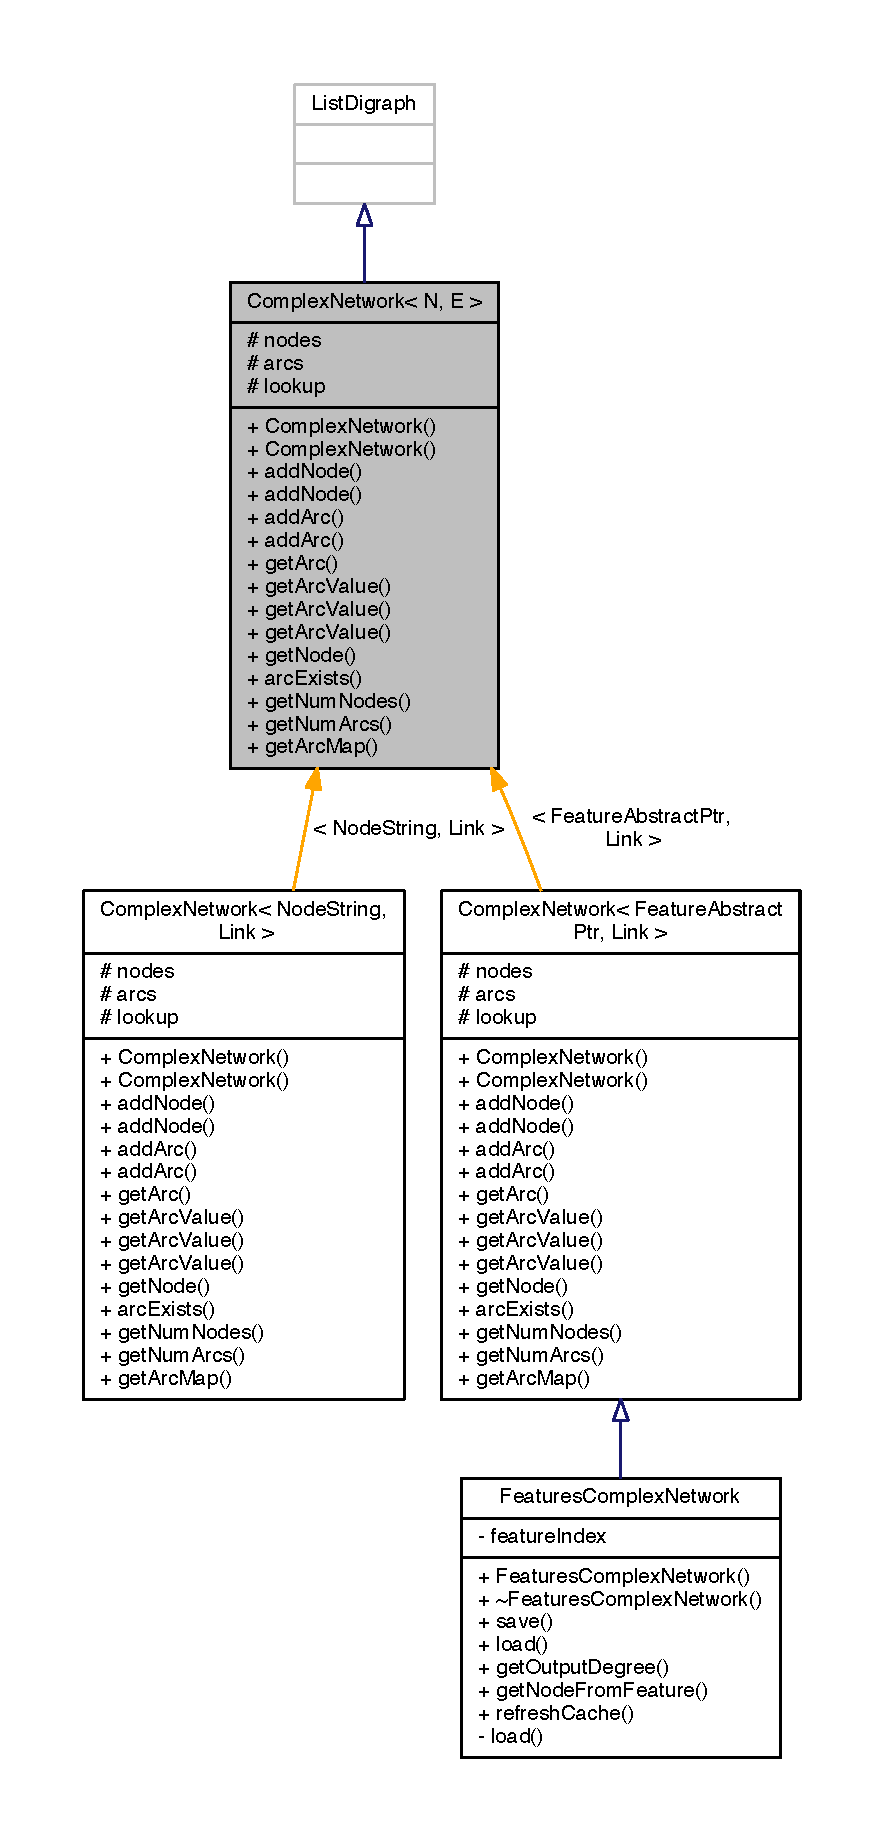
\includegraphics[width=254pt]{class_complex_network__inherit__graph}
\end{center}
\end{figure}


Collaboration diagram for Complex\+Network$<$ N\+O\+D\+E\+\_\+\+T\+Y\+P\+E, E\+D\+G\+E\+\_\+\+T\+Y\+P\+E $>$\+:\nopagebreak
\begin{figure}[H]
\begin{center}
\leavevmode
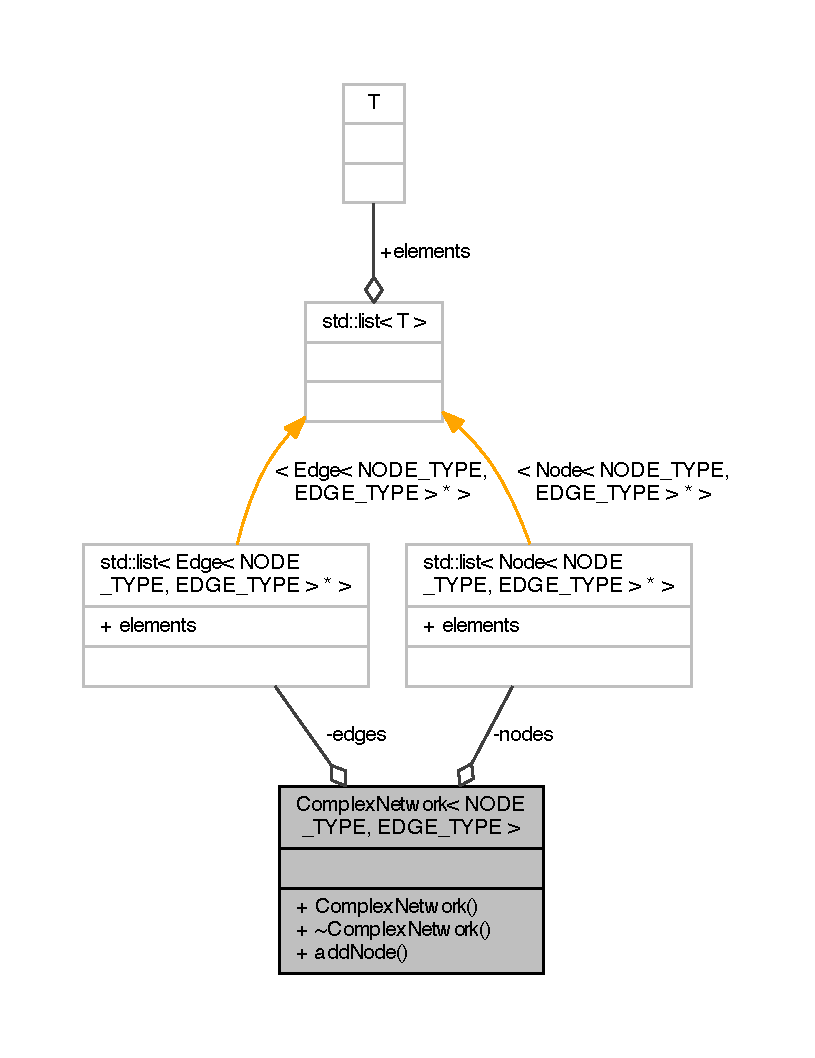
\includegraphics[width=350pt]{class_complex_network__coll__graph}
\end{center}
\end{figure}


\subsection{Constructor \& Destructor Documentation}
\hypertarget{class_complex_network_a4a16e825e1d8b487067ca21d677617a3}{\index{Complex\+Network@{Complex\+Network}!Complex\+Network@{Complex\+Network}}
\index{Complex\+Network@{Complex\+Network}!Complex\+Network@{Complex\+Network}}
\subsubsection[{Complex\+Network}]{\setlength{\rightskip}{0pt plus 5cm}template$<$typename N\+O\+D\+E\+\_\+\+T\+Y\+P\+E , typename E\+D\+G\+E\+\_\+\+T\+Y\+P\+E $>$ {\bf Complex\+Network}$<$ N\+O\+D\+E\+\_\+\+T\+Y\+P\+E, E\+D\+G\+E\+\_\+\+T\+Y\+P\+E $>$\+::{\bf Complex\+Network} (
\begin{DoxyParamCaption}
\item[{bool}]{directed = {\ttfamily true}}
\end{DoxyParamCaption}
)}}\label{class_complex_network_a4a16e825e1d8b487067ca21d677617a3}


\subsection{Member Function Documentation}
\hypertarget{class_complex_network_a52c25eb9c9c642a39681e4040fc0a17d}{\index{Complex\+Network@{Complex\+Network}!add\+Edge@{add\+Edge}}
\index{add\+Edge@{add\+Edge}!Complex\+Network@{Complex\+Network}}
\subsubsection[{add\+Edge}]{\setlength{\rightskip}{0pt plus 5cm}template$<$typename N\+O\+D\+E\+\_\+\+T\+Y\+P\+E , typename E\+D\+G\+E\+\_\+\+T\+Y\+P\+E$>$ void {\bf Complex\+Network}$<$ N\+O\+D\+E\+\_\+\+T\+Y\+P\+E, E\+D\+G\+E\+\_\+\+T\+Y\+P\+E $>$\+::add\+Edge (
\begin{DoxyParamCaption}
\item[{{\bf node\+\_\+id}}]{from, }
\item[{{\bf node\+\_\+id}}]{to, }
\item[{const E\+D\+G\+E\+\_\+\+T\+Y\+P\+E \&}]{e}
\end{DoxyParamCaption}
)\hspace{0.3cm}{\ttfamily [virtual]}}}\label{class_complex_network_a52c25eb9c9c642a39681e4040fc0a17d}


Here is the caller graph for this function\+:
\nopagebreak
\begin{figure}[H]
\begin{center}
\leavevmode
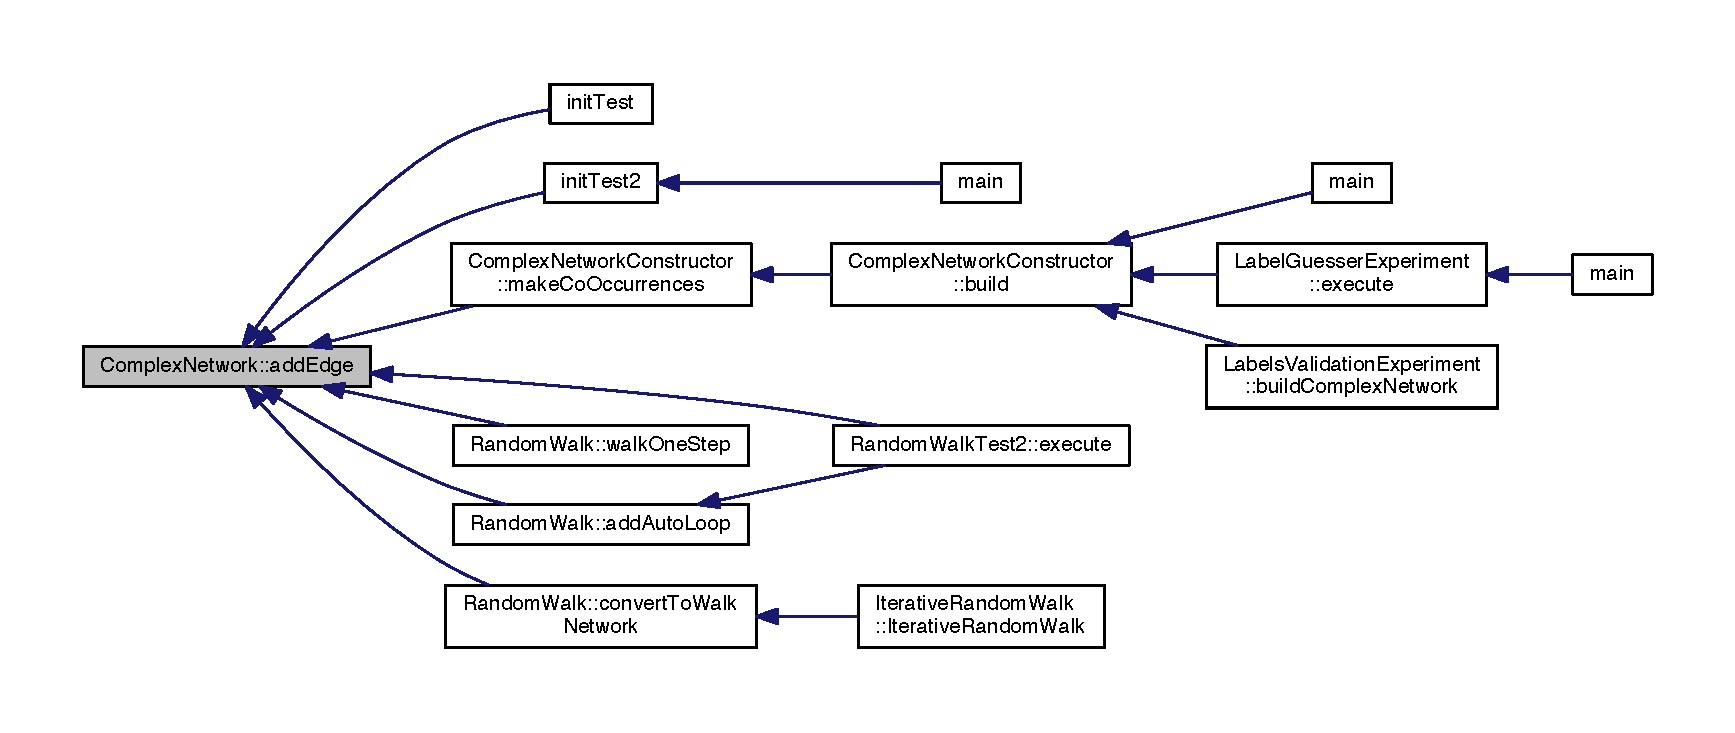
\includegraphics[width=350pt]{class_complex_network_a52c25eb9c9c642a39681e4040fc0a17d_icgraph}
\end{center}
\end{figure}


\hypertarget{class_complex_network_af2c31ca0d2142dafa1d88ca3ff22356f}{\index{Complex\+Network@{Complex\+Network}!add\+Node@{add\+Node}}
\index{add\+Node@{add\+Node}!Complex\+Network@{Complex\+Network}}
\subsubsection[{add\+Node}]{\setlength{\rightskip}{0pt plus 5cm}template$<$typename N\+O\+D\+E\+\_\+\+T\+Y\+P\+E, typename E\+D\+G\+E\+\_\+\+T\+Y\+P\+E $>$ {\bf node\+\_\+id} {\bf Complex\+Network}$<$ N\+O\+D\+E\+\_\+\+T\+Y\+P\+E, E\+D\+G\+E\+\_\+\+T\+Y\+P\+E $>$\+::add\+Node (
\begin{DoxyParamCaption}
\item[{const N\+O\+D\+E\+\_\+\+T\+Y\+P\+E \&}]{n}
\end{DoxyParamCaption}
)\hspace{0.3cm}{\ttfamily [virtual]}}}\label{class_complex_network_af2c31ca0d2142dafa1d88ca3ff22356f}


Reimplemented in \hyperlink{class_cached_complex_network_ad6e24699a050f5f2d7f908aba40b931c}{Cached\+Complex\+Network$<$ N\+O\+D\+E\+\_\+\+T\+Y\+P\+E, E\+D\+G\+E\+\_\+\+T\+Y\+P\+E $>$}, and \hyperlink{class_cached_complex_network_ad6e24699a050f5f2d7f908aba40b931c}{Cached\+Complex\+Network$<$ int, double $>$}.



Here is the caller graph for this function\+:
\nopagebreak
\begin{figure}[H]
\begin{center}
\leavevmode
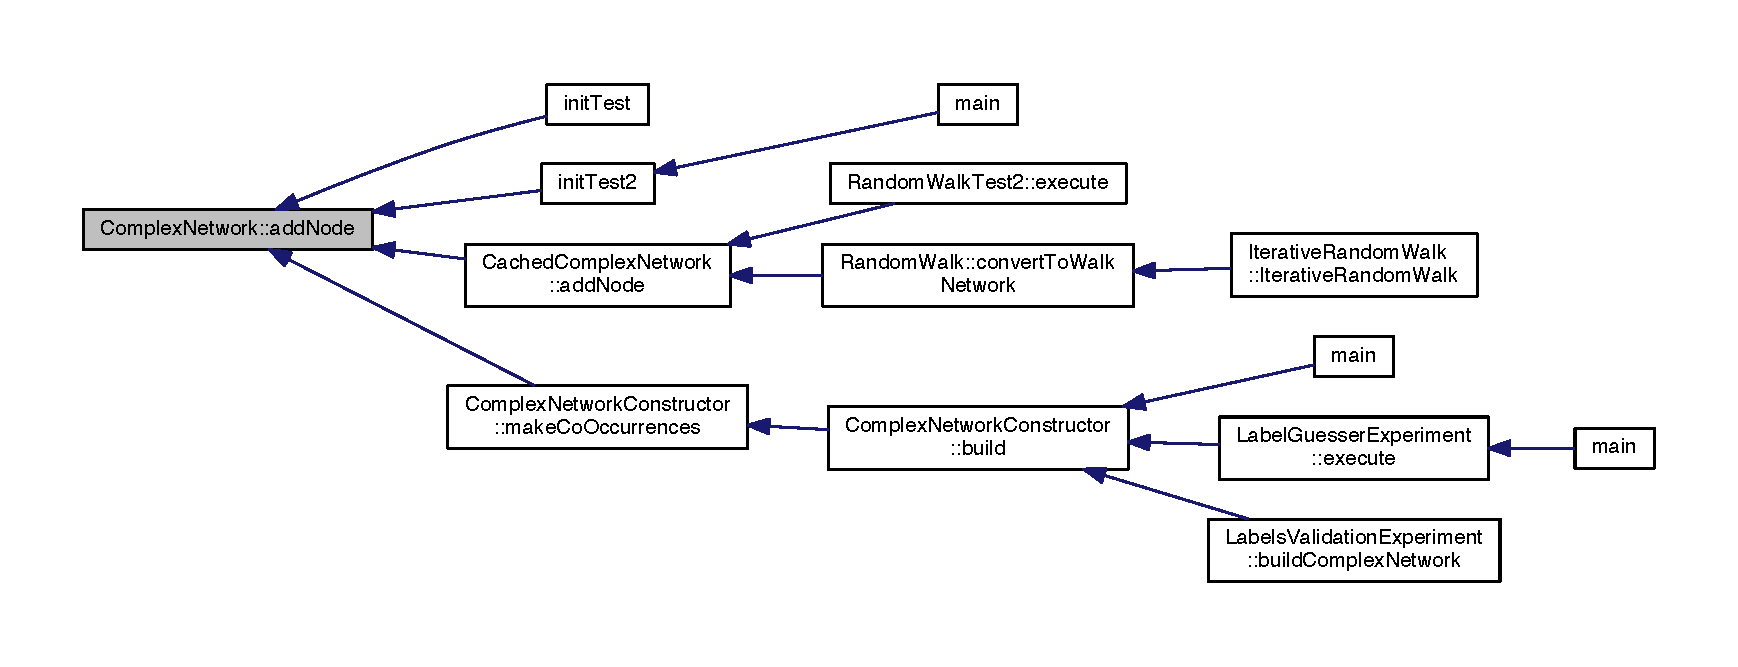
\includegraphics[width=350pt]{class_complex_network_af2c31ca0d2142dafa1d88ca3ff22356f_icgraph}
\end{center}
\end{figure}


\hypertarget{class_complex_network_ab02bc6912437322f146f6ce98b415759}{\index{Complex\+Network@{Complex\+Network}!Begin@{Begin}}
\index{Begin@{Begin}!Complex\+Network@{Complex\+Network}}
\subsubsection[{Begin}]{\setlength{\rightskip}{0pt plus 5cm}template$<$typename N\+O\+D\+E\+\_\+\+T\+Y\+P\+E , typename E\+D\+G\+E\+\_\+\+T\+Y\+P\+E $>$ {\bf Complex\+Network}$<$ N\+O\+D\+E\+\_\+\+T\+Y\+P\+E, E\+D\+G\+E\+\_\+\+T\+Y\+P\+E $>$\+::{\bf Node\+Iterator} {\bf Complex\+Network}$<$ N\+O\+D\+E\+\_\+\+T\+Y\+P\+E, E\+D\+G\+E\+\_\+\+T\+Y\+P\+E $>$\+::Begin (
\begin{DoxyParamCaption}
{}
\end{DoxyParamCaption}
)}}\label{class_complex_network_ab02bc6912437322f146f6ce98b415759}


Here is the caller graph for this function\+:
\nopagebreak
\begin{figure}[H]
\begin{center}
\leavevmode
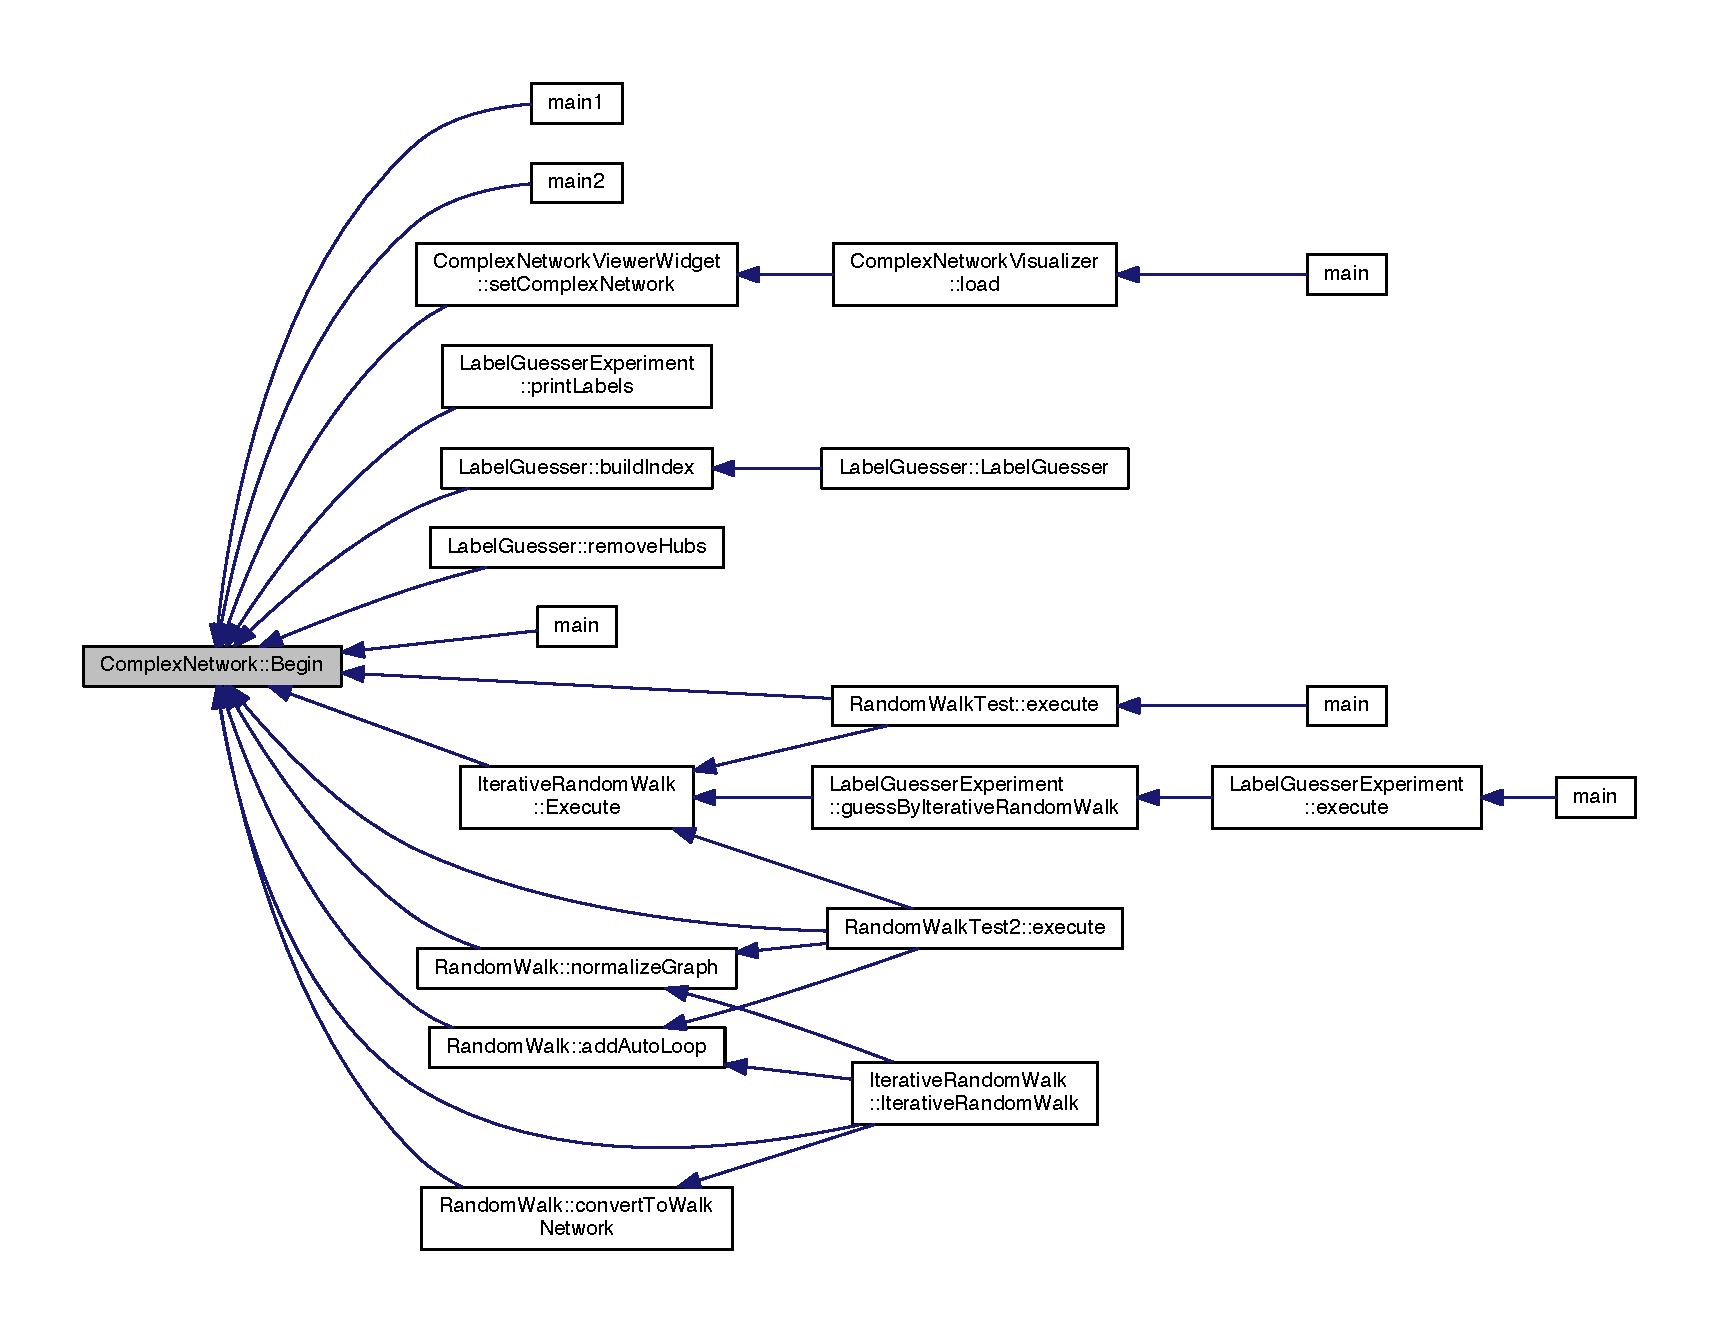
\includegraphics[width=350pt]{class_complex_network_ab02bc6912437322f146f6ce98b415759_icgraph}
\end{center}
\end{figure}


\hypertarget{class_complex_network_a64db5949375a84eba3d9ff559d68fc6e}{\index{Complex\+Network@{Complex\+Network}!clear@{clear}}
\index{clear@{clear}!Complex\+Network@{Complex\+Network}}
\subsubsection[{clear}]{\setlength{\rightskip}{0pt plus 5cm}template$<$typename N\+O\+D\+E\+\_\+\+T\+Y\+P\+E , typename E\+D\+G\+E\+\_\+\+T\+Y\+P\+E $>$ void {\bf Complex\+Network}$<$ N\+O\+D\+E\+\_\+\+T\+Y\+P\+E, E\+D\+G\+E\+\_\+\+T\+Y\+P\+E $>$\+::clear (
\begin{DoxyParamCaption}
{}
\end{DoxyParamCaption}
)\hspace{0.3cm}{\ttfamily [virtual]}}}\label{class_complex_network_a64db5949375a84eba3d9ff559d68fc6e}


Reimplemented in \hyperlink{class_features_complex_network_a747eba83de2a19a39e3d9f230d055d59}{Features\+Complex\+Network}.

\hypertarget{class_complex_network_a982b0db93143ff949025e326794af02d}{\index{Complex\+Network@{Complex\+Network}!create\+Edge\+Key@{create\+Edge\+Key}}
\index{create\+Edge\+Key@{create\+Edge\+Key}!Complex\+Network@{Complex\+Network}}
\subsubsection[{create\+Edge\+Key}]{\setlength{\rightskip}{0pt plus 5cm}template$<$typename N\+O\+D\+E\+\_\+\+T\+Y\+P\+E , typename E\+D\+G\+E\+\_\+\+T\+Y\+P\+E $>$ Q\+Pair$<$ {\bf node\+\_\+id}, {\bf node\+\_\+id} $>$ {\bf Complex\+Network}$<$ N\+O\+D\+E\+\_\+\+T\+Y\+P\+E, E\+D\+G\+E\+\_\+\+T\+Y\+P\+E $>$\+::create\+Edge\+Key (
\begin{DoxyParamCaption}
\item[{{\bf node\+\_\+id}}]{from, }
\item[{{\bf node\+\_\+id}}]{to}
\end{DoxyParamCaption}
)\hspace{0.3cm}{\ttfamily [inline]}, {\ttfamily [protected]}}}\label{class_complex_network_a982b0db93143ff949025e326794af02d}
\hypertarget{class_complex_network_a2167b224079f5c0b44443959ad0b6440}{\index{Complex\+Network@{Complex\+Network}!Edges\+Begin@{Edges\+Begin}}
\index{Edges\+Begin@{Edges\+Begin}!Complex\+Network@{Complex\+Network}}
\subsubsection[{Edges\+Begin}]{\setlength{\rightskip}{0pt plus 5cm}template$<$typename N\+O\+D\+E\+\_\+\+T\+Y\+P\+E , typename E\+D\+G\+E\+\_\+\+T\+Y\+P\+E $>$ {\bf Complex\+Network}$<$ N\+O\+D\+E\+\_\+\+T\+Y\+P\+E, E\+D\+G\+E\+\_\+\+T\+Y\+P\+E $>$\+::{\bf Edge\+Iterator} {\bf Complex\+Network}$<$ N\+O\+D\+E\+\_\+\+T\+Y\+P\+E, E\+D\+G\+E\+\_\+\+T\+Y\+P\+E $>$\+::Edges\+Begin (
\begin{DoxyParamCaption}
\item[{{\bf node\+\_\+id}}]{node\+\_\+from}
\end{DoxyParamCaption}
)}}\label{class_complex_network_a2167b224079f5c0b44443959ad0b6440}


Here is the caller graph for this function\+:\nopagebreak
\begin{figure}[H]
\begin{center}
\leavevmode
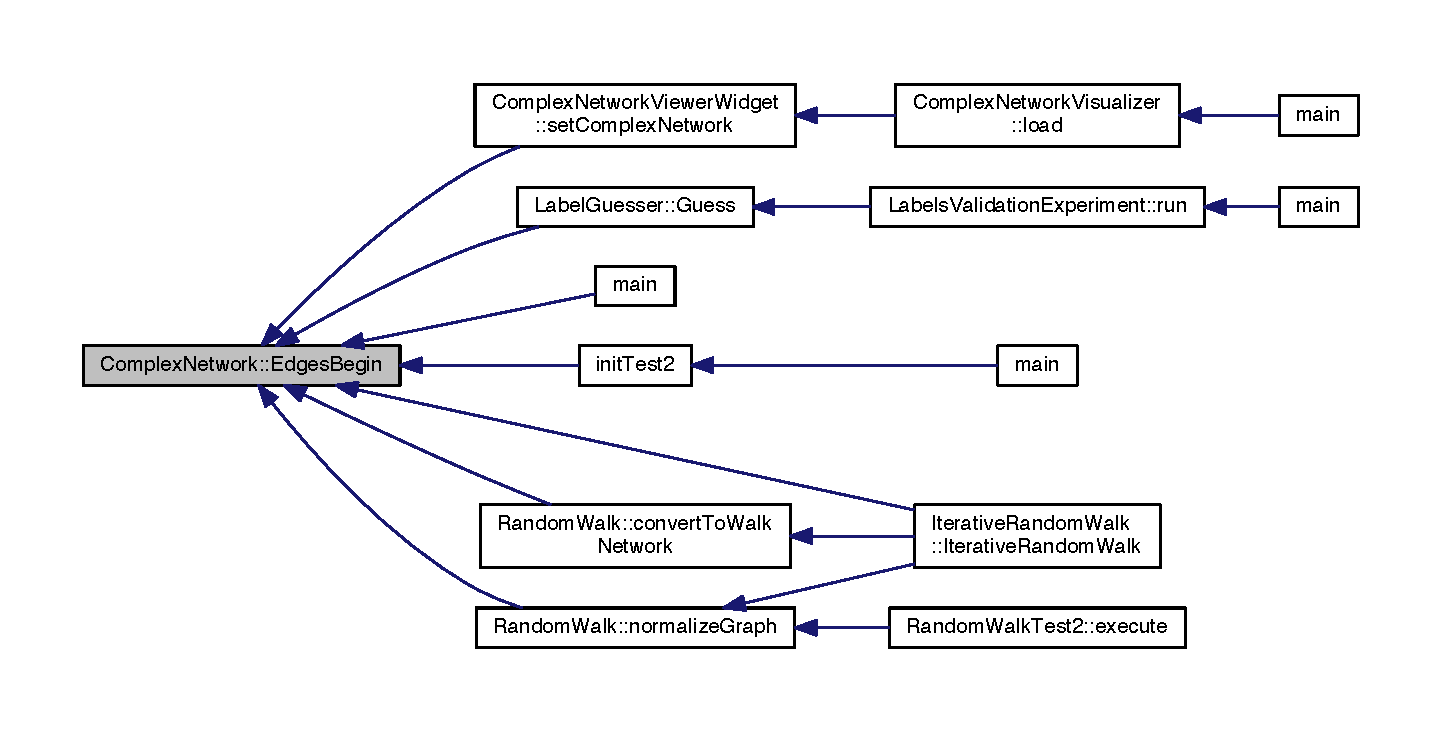
\includegraphics[width=350pt]{class_complex_network_a2167b224079f5c0b44443959ad0b6440_icgraph}
\end{center}
\end{figure}


\hypertarget{class_complex_network_a3a228b9a9497db2b9385deb4eb39f1e1}{\index{Complex\+Network@{Complex\+Network}!Edges\+Begin@{Edges\+Begin}}
\index{Edges\+Begin@{Edges\+Begin}!Complex\+Network@{Complex\+Network}}
\subsubsection[{Edges\+Begin}]{\setlength{\rightskip}{0pt plus 5cm}template$<$typename N\+O\+D\+E\+\_\+\+T\+Y\+P\+E , typename E\+D\+G\+E\+\_\+\+T\+Y\+P\+E $>$ {\bf Complex\+Network}$<$ N\+O\+D\+E\+\_\+\+T\+Y\+P\+E, E\+D\+G\+E\+\_\+\+T\+Y\+P\+E $>$\+::{\bf Edge\+Iterator} {\bf Complex\+Network}$<$ N\+O\+D\+E\+\_\+\+T\+Y\+P\+E, E\+D\+G\+E\+\_\+\+T\+Y\+P\+E $>$\+::Edges\+Begin (
\begin{DoxyParamCaption}
{}
\end{DoxyParamCaption}
)}}\label{class_complex_network_a3a228b9a9497db2b9385deb4eb39f1e1}
\hypertarget{class_complex_network_ad806138ea94ec18ed17f4681ab731208}{\index{Complex\+Network@{Complex\+Network}!Edges\+End@{Edges\+End}}
\index{Edges\+End@{Edges\+End}!Complex\+Network@{Complex\+Network}}
\subsubsection[{Edges\+End}]{\setlength{\rightskip}{0pt plus 5cm}template$<$typename N\+O\+D\+E\+\_\+\+T\+Y\+P\+E , typename E\+D\+G\+E\+\_\+\+T\+Y\+P\+E $>$ {\bf Complex\+Network}$<$ N\+O\+D\+E\+\_\+\+T\+Y\+P\+E, E\+D\+G\+E\+\_\+\+T\+Y\+P\+E $>$\+::{\bf Edge\+Iterator} {\bf Complex\+Network}$<$ N\+O\+D\+E\+\_\+\+T\+Y\+P\+E, E\+D\+G\+E\+\_\+\+T\+Y\+P\+E $>$\+::Edges\+End (
\begin{DoxyParamCaption}
\item[{{\bf node\+\_\+id}}]{node\+\_\+from}
\end{DoxyParamCaption}
)}}\label{class_complex_network_ad806138ea94ec18ed17f4681ab731208}


Here is the caller graph for this function\+:\nopagebreak
\begin{figure}[H]
\begin{center}
\leavevmode
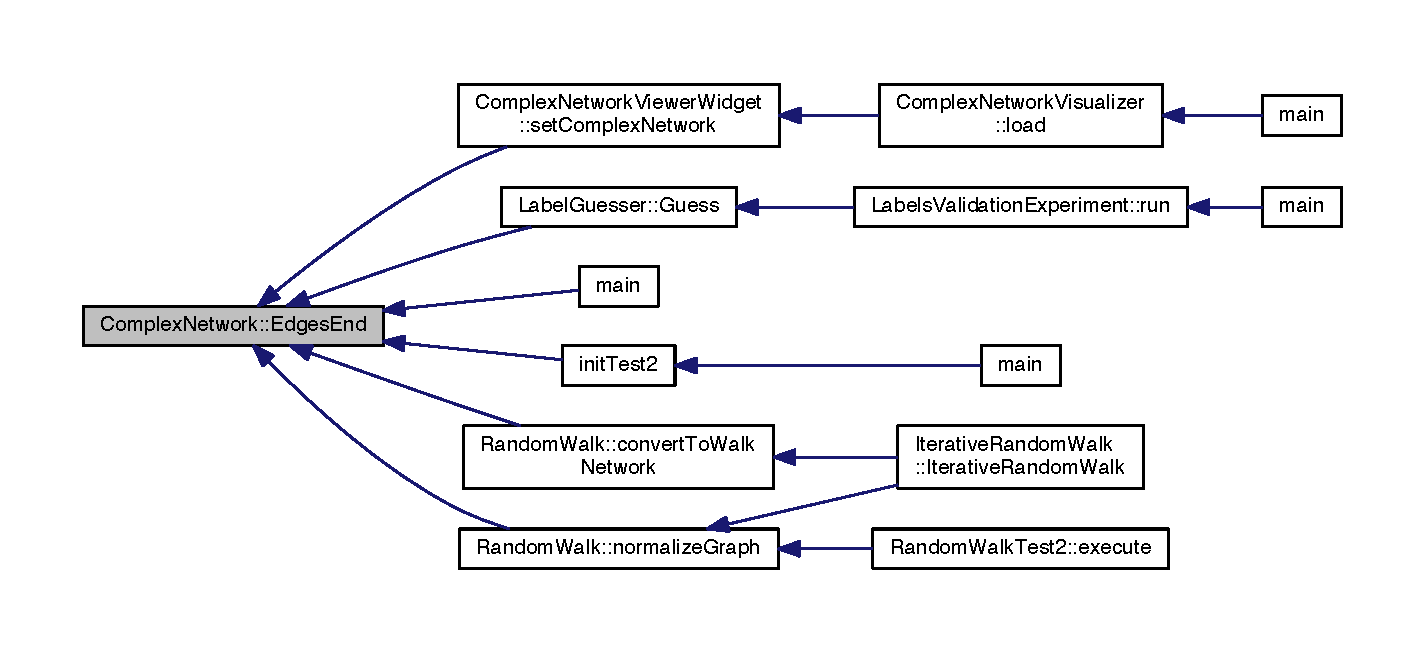
\includegraphics[width=350pt]{class_complex_network_ad806138ea94ec18ed17f4681ab731208_icgraph}
\end{center}
\end{figure}


\hypertarget{class_complex_network_afa7d628b66a815d97afbf5373640d12b}{\index{Complex\+Network@{Complex\+Network}!Edges\+End@{Edges\+End}}
\index{Edges\+End@{Edges\+End}!Complex\+Network@{Complex\+Network}}
\subsubsection[{Edges\+End}]{\setlength{\rightskip}{0pt plus 5cm}template$<$typename N\+O\+D\+E\+\_\+\+T\+Y\+P\+E , typename E\+D\+G\+E\+\_\+\+T\+Y\+P\+E $>$ {\bf Complex\+Network}$<$ N\+O\+D\+E\+\_\+\+T\+Y\+P\+E, E\+D\+G\+E\+\_\+\+T\+Y\+P\+E $>$\+::{\bf Edge\+Iterator} {\bf Complex\+Network}$<$ N\+O\+D\+E\+\_\+\+T\+Y\+P\+E, E\+D\+G\+E\+\_\+\+T\+Y\+P\+E $>$\+::Edges\+End (
\begin{DoxyParamCaption}
{}
\end{DoxyParamCaption}
)}}\label{class_complex_network_afa7d628b66a815d97afbf5373640d12b}
\hypertarget{class_complex_network_a2c90f4efd046776d7a53776b24daae0f}{\index{Complex\+Network@{Complex\+Network}!End@{End}}
\index{End@{End}!Complex\+Network@{Complex\+Network}}
\subsubsection[{End}]{\setlength{\rightskip}{0pt plus 5cm}template$<$typename N\+O\+D\+E\+\_\+\+T\+Y\+P\+E , typename E\+D\+G\+E\+\_\+\+T\+Y\+P\+E $>$ {\bf Complex\+Network}$<$ N\+O\+D\+E\+\_\+\+T\+Y\+P\+E, E\+D\+G\+E\+\_\+\+T\+Y\+P\+E $>$\+::{\bf Node\+Iterator} {\bf Complex\+Network}$<$ N\+O\+D\+E\+\_\+\+T\+Y\+P\+E, E\+D\+G\+E\+\_\+\+T\+Y\+P\+E $>$\+::End (
\begin{DoxyParamCaption}
{}
\end{DoxyParamCaption}
)}}\label{class_complex_network_a2c90f4efd046776d7a53776b24daae0f}


Here is the caller graph for this function\+:
\nopagebreak
\begin{figure}[H]
\begin{center}
\leavevmode
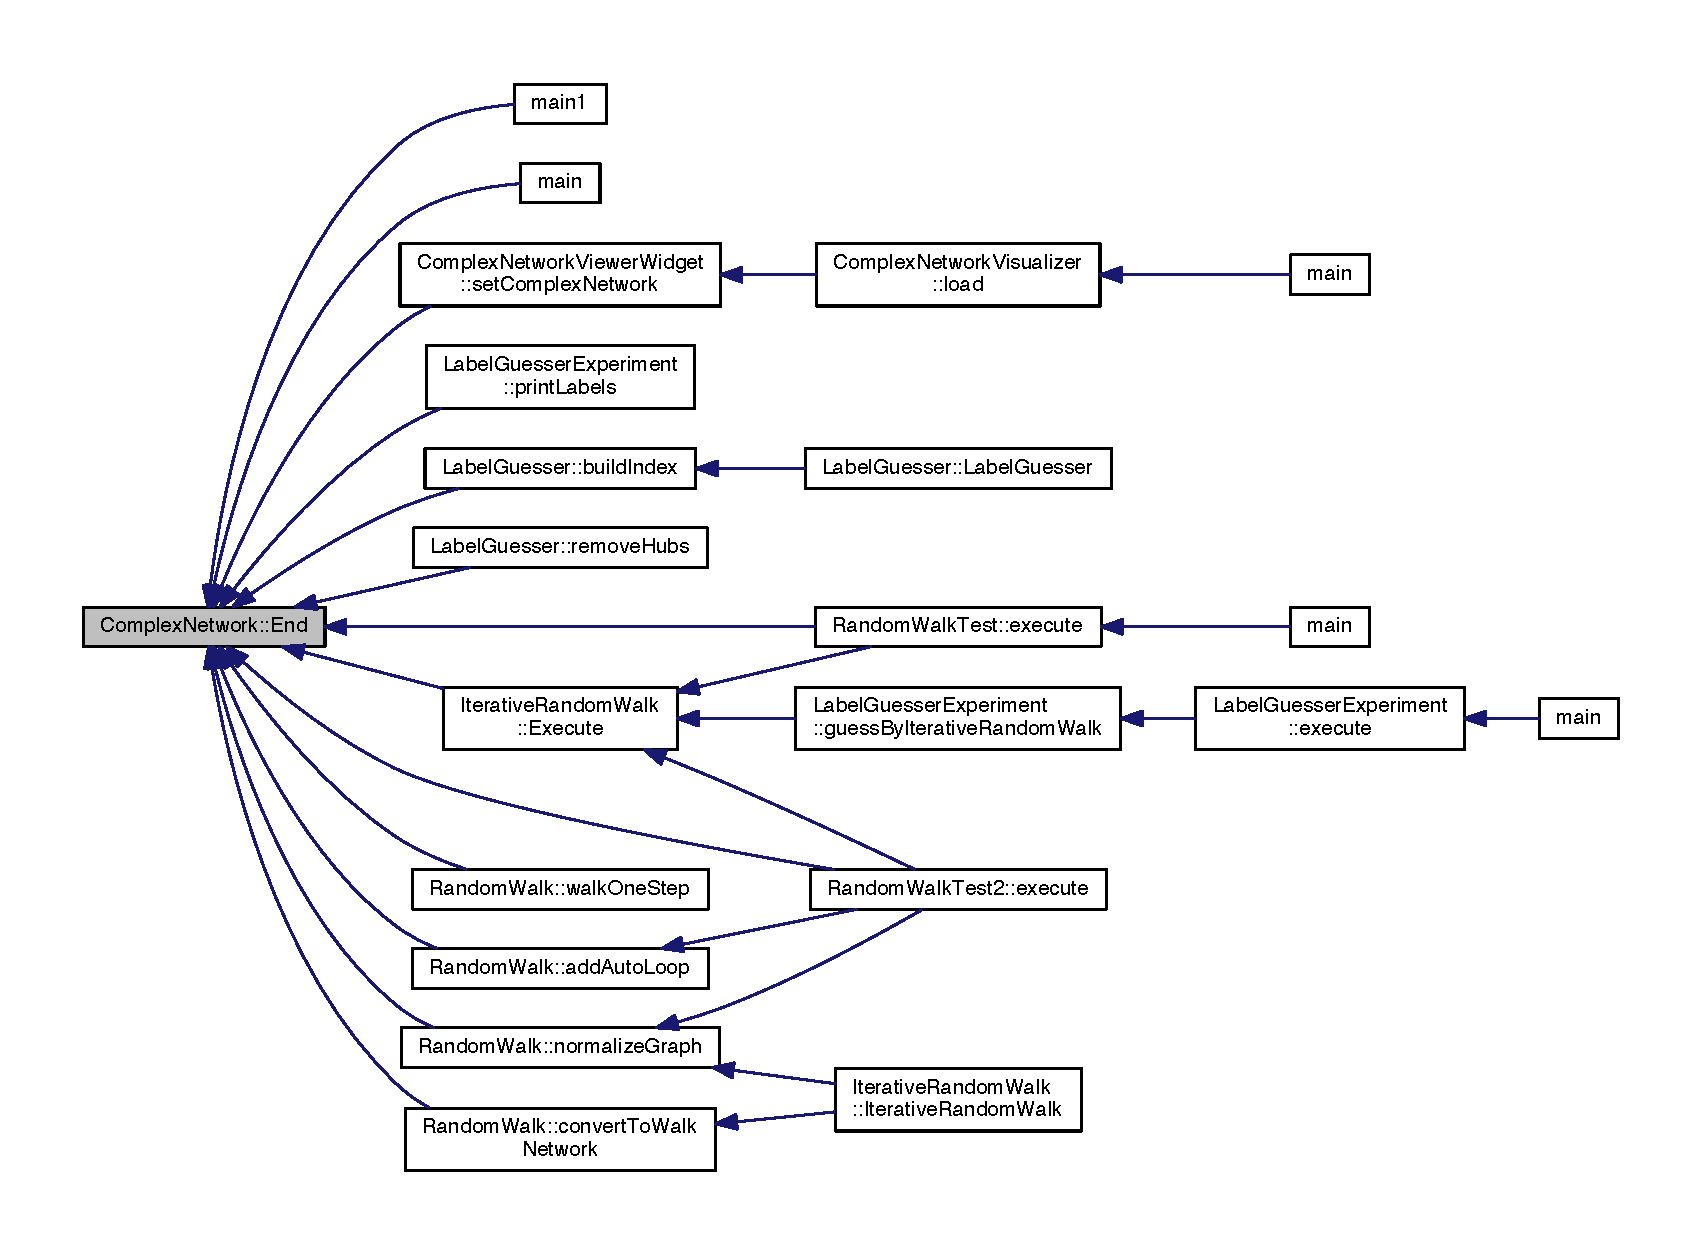
\includegraphics[width=350pt]{class_complex_network_a2c90f4efd046776d7a53776b24daae0f_icgraph}
\end{center}
\end{figure}


\hypertarget{class_complex_network_a6a1c638e4604efe06c12ce3065020ec1}{\index{Complex\+Network@{Complex\+Network}!get\+Edge@{get\+Edge}}
\index{get\+Edge@{get\+Edge}!Complex\+Network@{Complex\+Network}}
\subsubsection[{get\+Edge}]{\setlength{\rightskip}{0pt plus 5cm}template$<$typename N\+O\+D\+E\+\_\+\+T\+Y\+P\+E , typename E\+D\+G\+E\+\_\+\+T\+Y\+P\+E $>$ E\+D\+G\+E\+\_\+\+T\+Y\+P\+E $\ast$ {\bf Complex\+Network}$<$ N\+O\+D\+E\+\_\+\+T\+Y\+P\+E, E\+D\+G\+E\+\_\+\+T\+Y\+P\+E $>$\+::get\+Edge (
\begin{DoxyParamCaption}
\item[{{\bf node\+\_\+id}}]{from, }
\item[{{\bf node\+\_\+id}}]{to}
\end{DoxyParamCaption}
)\hspace{0.3cm}{\ttfamily [virtual]}}}\label{class_complex_network_a6a1c638e4604efe06c12ce3065020ec1}


Here is the caller graph for this function\+:
\nopagebreak
\begin{figure}[H]
\begin{center}
\leavevmode
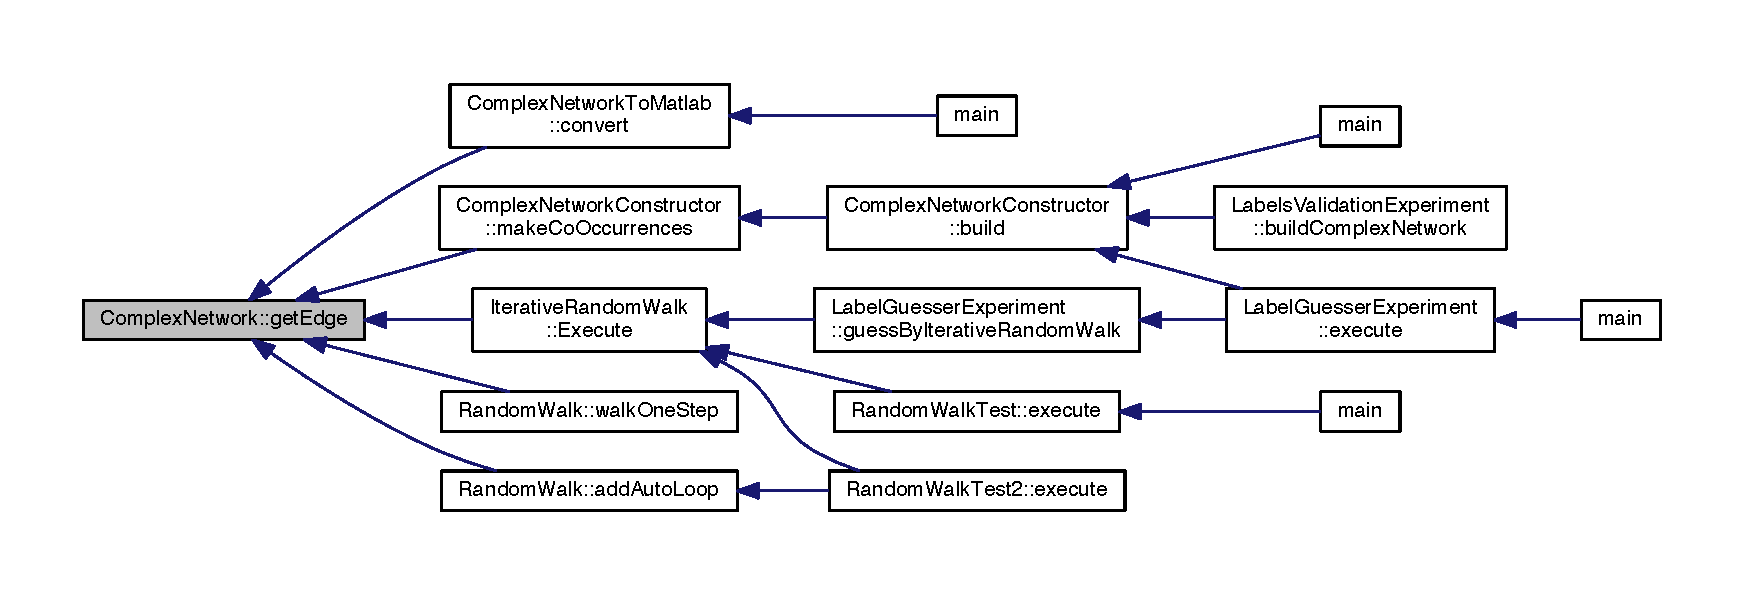
\includegraphics[width=350pt]{class_complex_network_a6a1c638e4604efe06c12ce3065020ec1_icgraph}
\end{center}
\end{figure}


\hypertarget{class_complex_network_ad440008416fc33500754d77b2532560f}{\index{Complex\+Network@{Complex\+Network}!get\+Edge\+From\+Edge\+Id@{get\+Edge\+From\+Edge\+Id}}
\index{get\+Edge\+From\+Edge\+Id@{get\+Edge\+From\+Edge\+Id}!Complex\+Network@{Complex\+Network}}
\subsubsection[{get\+Edge\+From\+Edge\+Id}]{\setlength{\rightskip}{0pt plus 5cm}template$<$typename N\+O\+D\+E\+\_\+\+T\+Y\+P\+E , typename E\+D\+G\+E\+\_\+\+T\+Y\+P\+E $>$ E\+D\+G\+E\+\_\+\+T\+Y\+P\+E $\ast$ {\bf Complex\+Network}$<$ N\+O\+D\+E\+\_\+\+T\+Y\+P\+E, E\+D\+G\+E\+\_\+\+T\+Y\+P\+E $>$\+::get\+Edge\+From\+Edge\+Id (
\begin{DoxyParamCaption}
\item[{{\bf edge\+\_\+id}}]{id}
\end{DoxyParamCaption}
)\hspace{0.3cm}{\ttfamily [virtual]}}}\label{class_complex_network_ad440008416fc33500754d77b2532560f}
\hypertarget{class_complex_network_a3711aff250a942a9ad61d0571be82c43}{\index{Complex\+Network@{Complex\+Network}!get\+Node@{get\+Node}}
\index{get\+Node@{get\+Node}!Complex\+Network@{Complex\+Network}}
\subsubsection[{get\+Node}]{\setlength{\rightskip}{0pt plus 5cm}template$<$typename N\+O\+D\+E\+\_\+\+T\+Y\+P\+E , typename E\+D\+G\+E\+\_\+\+T\+Y\+P\+E $>$ N\+O\+D\+E\+\_\+\+T\+Y\+P\+E $\ast$ {\bf Complex\+Network}$<$ N\+O\+D\+E\+\_\+\+T\+Y\+P\+E, E\+D\+G\+E\+\_\+\+T\+Y\+P\+E $>$\+::get\+Node (
\begin{DoxyParamCaption}
\item[{{\bf node\+\_\+id}}]{id}
\end{DoxyParamCaption}
)\hspace{0.3cm}{\ttfamily [virtual]}}}\label{class_complex_network_a3711aff250a942a9ad61d0571be82c43}


Here is the caller graph for this function\+:
\nopagebreak
\begin{figure}[H]
\begin{center}
\leavevmode
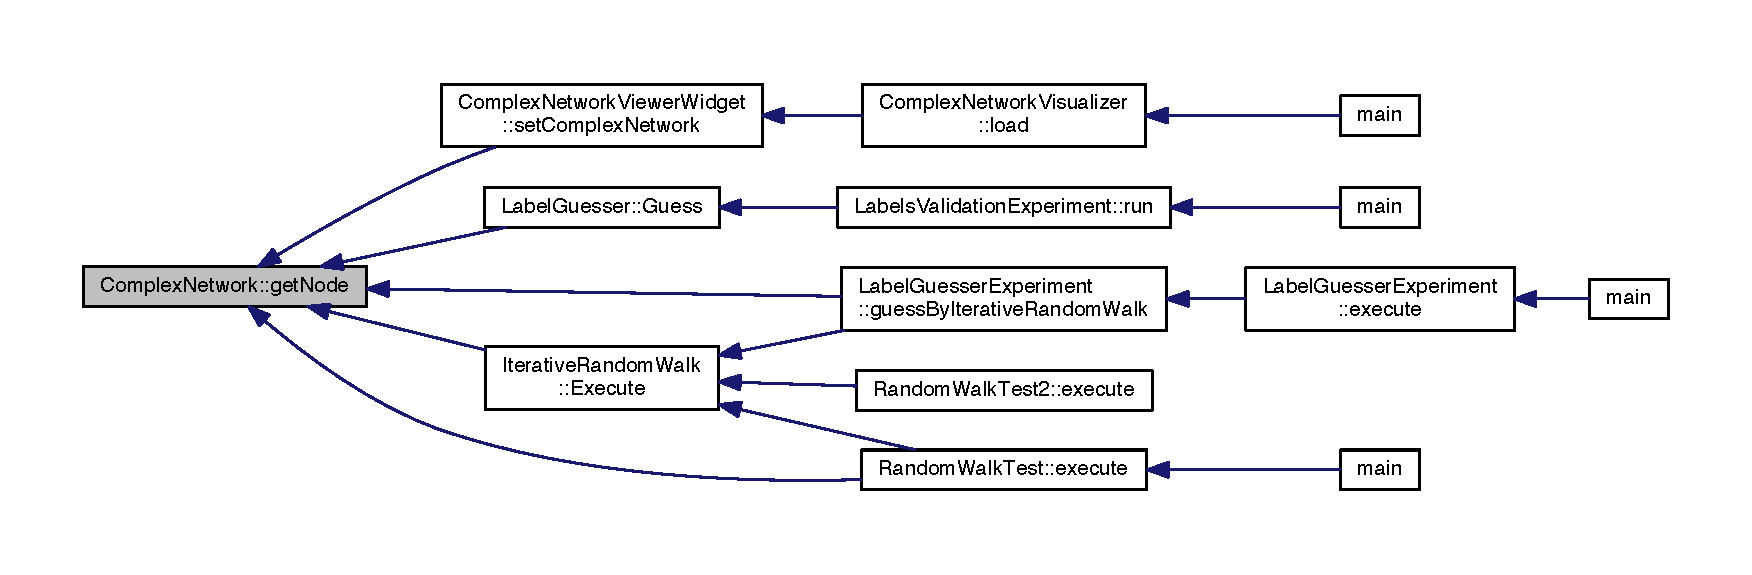
\includegraphics[width=350pt]{class_complex_network_a3711aff250a942a9ad61d0571be82c43_icgraph}
\end{center}
\end{figure}


\hypertarget{class_complex_network_a720cb4e40342648d394792cc693d29a5}{\index{Complex\+Network@{Complex\+Network}!get\+Num\+Edges@{get\+Num\+Edges}}
\index{get\+Num\+Edges@{get\+Num\+Edges}!Complex\+Network@{Complex\+Network}}
\subsubsection[{get\+Num\+Edges}]{\setlength{\rightskip}{0pt plus 5cm}template$<$typename N\+O\+D\+E\+\_\+\+T\+Y\+P\+E , typename E\+D\+G\+E\+\_\+\+T\+Y\+P\+E $>$ unsigned int {\bf Complex\+Network}$<$ N\+O\+D\+E\+\_\+\+T\+Y\+P\+E, E\+D\+G\+E\+\_\+\+T\+Y\+P\+E $>$\+::get\+Num\+Edges (
\begin{DoxyParamCaption}
{}
\end{DoxyParamCaption}
) const}}\label{class_complex_network_a720cb4e40342648d394792cc693d29a5}


Here is the caller graph for this function\+:\nopagebreak
\begin{figure}[H]
\begin{center}
\leavevmode
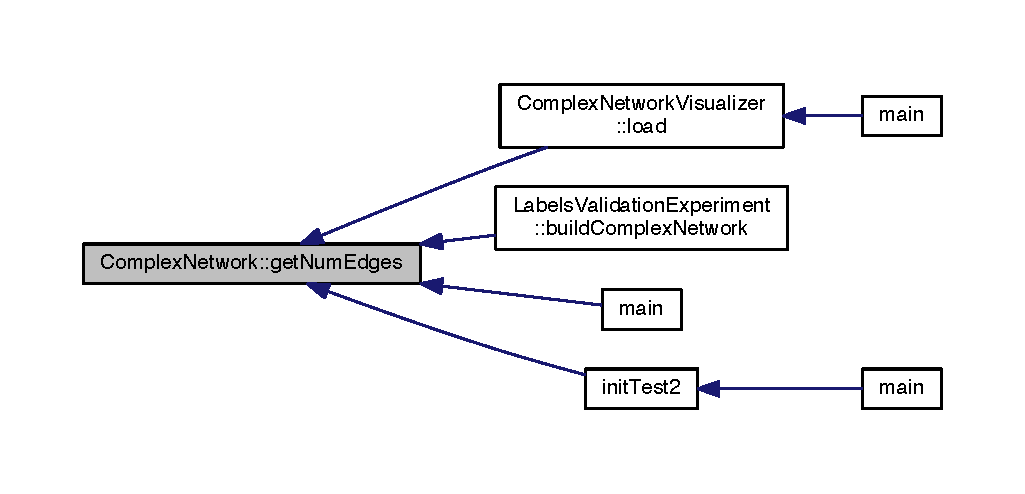
\includegraphics[width=350pt]{class_complex_network_a720cb4e40342648d394792cc693d29a5_icgraph}
\end{center}
\end{figure}


\hypertarget{class_complex_network_a4036d2cda2dc5596d03e164c3455aff6}{\index{Complex\+Network@{Complex\+Network}!get\+Num\+Edges@{get\+Num\+Edges}}
\index{get\+Num\+Edges@{get\+Num\+Edges}!Complex\+Network@{Complex\+Network}}
\subsubsection[{get\+Num\+Edges}]{\setlength{\rightskip}{0pt plus 5cm}template$<$typename N\+O\+D\+E\+\_\+\+T\+Y\+P\+E , typename E\+D\+G\+E\+\_\+\+T\+Y\+P\+E $>$ unsigned int {\bf Complex\+Network}$<$ N\+O\+D\+E\+\_\+\+T\+Y\+P\+E, E\+D\+G\+E\+\_\+\+T\+Y\+P\+E $>$\+::get\+Num\+Edges (
\begin{DoxyParamCaption}
\item[{{\bf node\+\_\+id}}]{id}
\end{DoxyParamCaption}
) const}}\label{class_complex_network_a4036d2cda2dc5596d03e164c3455aff6}
\hypertarget{class_complex_network_afee98f26ceed674c17be01a740787170}{\index{Complex\+Network@{Complex\+Network}!get\+Num\+Nodes@{get\+Num\+Nodes}}
\index{get\+Num\+Nodes@{get\+Num\+Nodes}!Complex\+Network@{Complex\+Network}}
\subsubsection[{get\+Num\+Nodes}]{\setlength{\rightskip}{0pt plus 5cm}template$<$typename N\+O\+D\+E\+\_\+\+T\+Y\+P\+E , typename E\+D\+G\+E\+\_\+\+T\+Y\+P\+E $>$ unsigned int {\bf Complex\+Network}$<$ N\+O\+D\+E\+\_\+\+T\+Y\+P\+E, E\+D\+G\+E\+\_\+\+T\+Y\+P\+E $>$\+::get\+Num\+Nodes (
\begin{DoxyParamCaption}
{}
\end{DoxyParamCaption}
) const}}\label{class_complex_network_afee98f26ceed674c17be01a740787170}


Here is the caller graph for this function\+:
\nopagebreak
\begin{figure}[H]
\begin{center}
\leavevmode
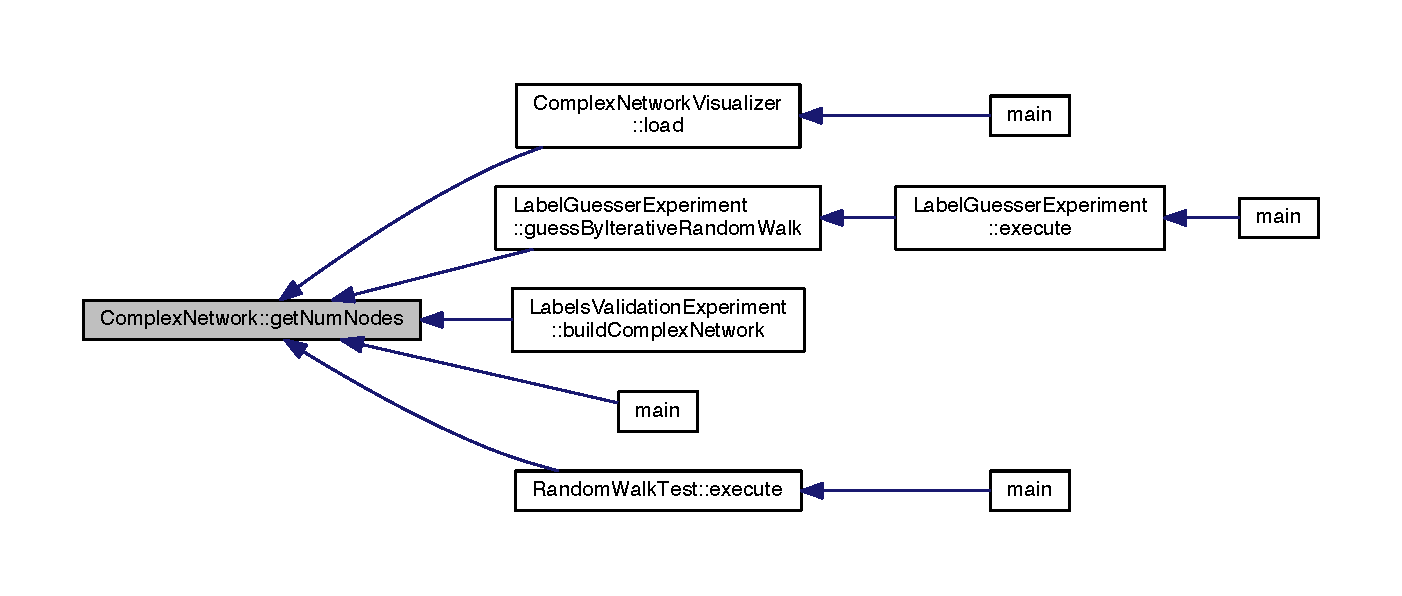
\includegraphics[width=350pt]{class_complex_network_afee98f26ceed674c17be01a740787170_icgraph}
\end{center}
\end{figure}


\hypertarget{class_complex_network_a54fbdb35418f424e8dad0dbc5dc16bee}{\index{Complex\+Network@{Complex\+Network}!load@{load}}
\index{load@{load}!Complex\+Network@{Complex\+Network}}
\subsubsection[{load}]{\setlength{\rightskip}{0pt plus 5cm}template$<$typename N\+O\+D\+E\+\_\+\+T\+Y\+P\+E , typename E\+D\+G\+E\+\_\+\+T\+Y\+P\+E $>$ void {\bf Complex\+Network}$<$ N\+O\+D\+E\+\_\+\+T\+Y\+P\+E, E\+D\+G\+E\+\_\+\+T\+Y\+P\+E $>$\+::load (
\begin{DoxyParamCaption}
\item[{const char $\ast$}]{filename}
\end{DoxyParamCaption}
)}}\label{class_complex_network_a54fbdb35418f424e8dad0dbc5dc16bee}


Here is the caller graph for this function\+:\nopagebreak
\begin{figure}[H]
\begin{center}
\leavevmode
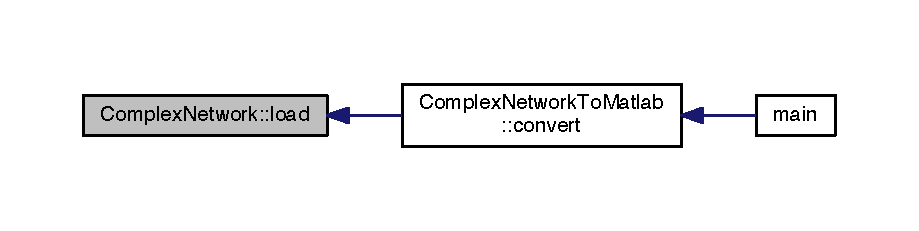
\includegraphics[width=350pt]{class_complex_network_a54fbdb35418f424e8dad0dbc5dc16bee_icgraph}
\end{center}
\end{figure}


\hypertarget{class_complex_network_a5a8b07f5ca5d247e13a2e2bc5ac75de1}{\index{Complex\+Network@{Complex\+Network}!operator=@{operator=}}
\index{operator=@{operator=}!Complex\+Network@{Complex\+Network}}
\subsubsection[{operator=}]{\setlength{\rightskip}{0pt plus 5cm}template$<$typename N\+O\+D\+E\+\_\+\+T\+Y\+P\+E, typename E\+D\+G\+E\+\_\+\+T\+Y\+P\+E$>$ {\bf Complex\+Network}$<$ N\+O\+D\+E\+\_\+\+T\+Y\+P\+E, E\+D\+G\+E\+\_\+\+T\+Y\+P\+E $>$ \& {\bf Complex\+Network}$<$ N\+O\+D\+E\+\_\+\+T\+Y\+P\+E, E\+D\+G\+E\+\_\+\+T\+Y\+P\+E $>$\+::operator= (
\begin{DoxyParamCaption}
\item[{const {\bf Complex\+Network}$<$ N\+O\+D\+E\+\_\+\+T\+Y\+P\+E, E\+D\+G\+E\+\_\+\+T\+Y\+P\+E $>$ \&}]{cn}
\end{DoxyParamCaption}
)}}\label{class_complex_network_a5a8b07f5ca5d247e13a2e2bc5ac75de1}
\hypertarget{class_complex_network_a9b2c7df561a2ad5fc14b04a5c5c56828}{\index{Complex\+Network@{Complex\+Network}!remove\+Edge@{remove\+Edge}}
\index{remove\+Edge@{remove\+Edge}!Complex\+Network@{Complex\+Network}}
\subsubsection[{remove\+Edge}]{\setlength{\rightskip}{0pt plus 5cm}template$<$typename N\+O\+D\+E\+\_\+\+T\+Y\+P\+E , typename E\+D\+G\+E\+\_\+\+T\+Y\+P\+E $>$ bool {\bf Complex\+Network}$<$ N\+O\+D\+E\+\_\+\+T\+Y\+P\+E, E\+D\+G\+E\+\_\+\+T\+Y\+P\+E $>$\+::remove\+Edge (
\begin{DoxyParamCaption}
\item[{{\bf node\+\_\+id}}]{from, }
\item[{{\bf node\+\_\+id}}]{to}
\end{DoxyParamCaption}
)\hspace{0.3cm}{\ttfamily [virtual]}}}\label{class_complex_network_a9b2c7df561a2ad5fc14b04a5c5c56828}


Here is the caller graph for this function\+:\nopagebreak
\begin{figure}[H]
\begin{center}
\leavevmode
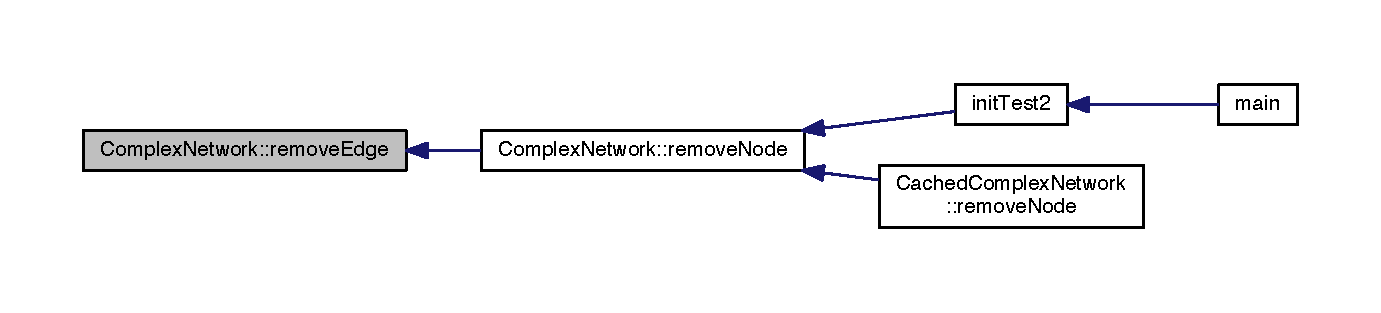
\includegraphics[width=350pt]{class_complex_network_a9b2c7df561a2ad5fc14b04a5c5c56828_icgraph}
\end{center}
\end{figure}


\hypertarget{class_complex_network_a33f2b4528cc31296ede98be7e6dcd600}{\index{Complex\+Network@{Complex\+Network}!remove\+Node@{remove\+Node}}
\index{remove\+Node@{remove\+Node}!Complex\+Network@{Complex\+Network}}
\subsubsection[{remove\+Node}]{\setlength{\rightskip}{0pt plus 5cm}template$<$typename N\+O\+D\+E\+\_\+\+T\+Y\+P\+E , typename E\+D\+G\+E\+\_\+\+T\+Y\+P\+E $>$ bool {\bf Complex\+Network}$<$ N\+O\+D\+E\+\_\+\+T\+Y\+P\+E, E\+D\+G\+E\+\_\+\+T\+Y\+P\+E $>$\+::remove\+Node (
\begin{DoxyParamCaption}
\item[{{\bf node\+\_\+id}}]{id}
\end{DoxyParamCaption}
)\hspace{0.3cm}{\ttfamily [virtual]}}}\label{class_complex_network_a33f2b4528cc31296ede98be7e6dcd600}


Reimplemented in \hyperlink{class_cached_complex_network_a800aa02b94aa4bb73227e139cb246ddf}{Cached\+Complex\+Network$<$ N\+O\+D\+E\+\_\+\+T\+Y\+P\+E, E\+D\+G\+E\+\_\+\+T\+Y\+P\+E $>$}, and \hyperlink{class_cached_complex_network_a800aa02b94aa4bb73227e139cb246ddf}{Cached\+Complex\+Network$<$ int, double $>$}.



Here is the call graph for this function\+:\nopagebreak
\begin{figure}[H]
\begin{center}
\leavevmode
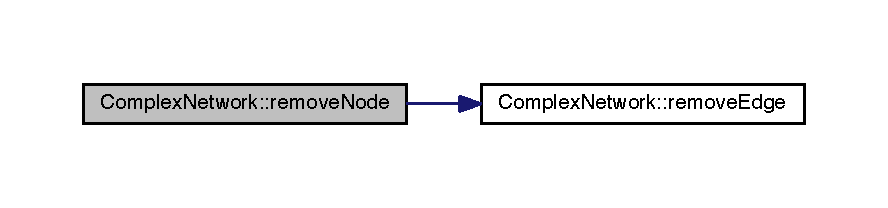
\includegraphics[width=350pt]{class_complex_network_a33f2b4528cc31296ede98be7e6dcd600_cgraph}
\end{center}
\end{figure}




Here is the caller graph for this function\+:\nopagebreak
\begin{figure}[H]
\begin{center}
\leavevmode
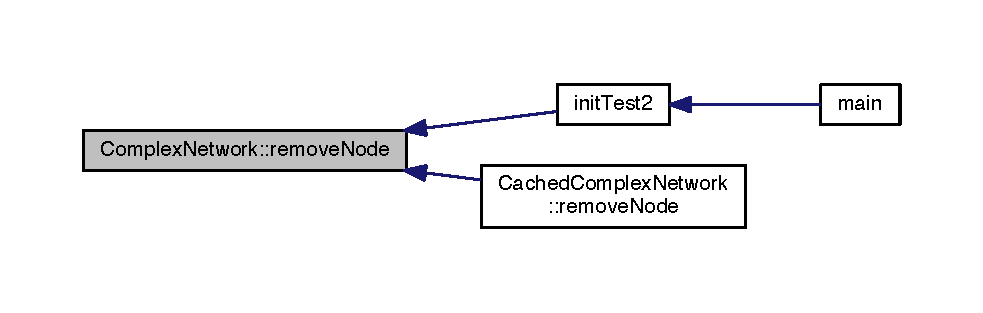
\includegraphics[width=350pt]{class_complex_network_a33f2b4528cc31296ede98be7e6dcd600_icgraph}
\end{center}
\end{figure}


\hypertarget{class_complex_network_a5d127d4296808b7ccdadccaa58084e96}{\index{Complex\+Network@{Complex\+Network}!save@{save}}
\index{save@{save}!Complex\+Network@{Complex\+Network}}
\subsubsection[{save}]{\setlength{\rightskip}{0pt plus 5cm}template$<$typename N\+O\+D\+E\+\_\+\+T\+Y\+P\+E , typename E\+D\+G\+E\+\_\+\+T\+Y\+P\+E $>$ void {\bf Complex\+Network}$<$ N\+O\+D\+E\+\_\+\+T\+Y\+P\+E, E\+D\+G\+E\+\_\+\+T\+Y\+P\+E $>$\+::save (
\begin{DoxyParamCaption}
\item[{const char $\ast$}]{filename}
\end{DoxyParamCaption}
)}}\label{class_complex_network_a5d127d4296808b7ccdadccaa58084e96}


Here is the caller graph for this function\+:\nopagebreak
\begin{figure}[H]
\begin{center}
\leavevmode
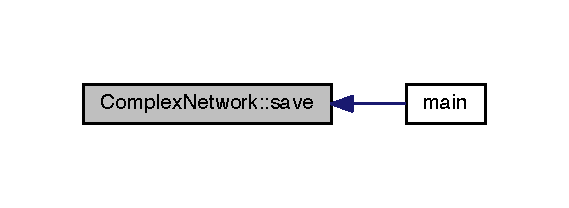
\includegraphics[width=273pt]{class_complex_network_a5d127d4296808b7ccdadccaa58084e96_icgraph}
\end{center}
\end{figure}




\subsection{Member Data Documentation}
\hypertarget{class_complex_network_a5305dba65a6d949064e46a6729c39e53}{\index{Complex\+Network@{Complex\+Network}!current\+\_\+edge\+\_\+id@{current\+\_\+edge\+\_\+id}}
\index{current\+\_\+edge\+\_\+id@{current\+\_\+edge\+\_\+id}!Complex\+Network@{Complex\+Network}}
\subsubsection[{current\+\_\+edge\+\_\+id}]{\setlength{\rightskip}{0pt plus 5cm}template$<$typename N\+O\+D\+E\+\_\+\+T\+Y\+P\+E, typename E\+D\+G\+E\+\_\+\+T\+Y\+P\+E$>$ {\bf edge\+\_\+id} {\bf Complex\+Network}$<$ N\+O\+D\+E\+\_\+\+T\+Y\+P\+E, E\+D\+G\+E\+\_\+\+T\+Y\+P\+E $>$\+::current\+\_\+edge\+\_\+id\hspace{0.3cm}{\ttfamily [protected]}}}\label{class_complex_network_a5305dba65a6d949064e46a6729c39e53}
\hypertarget{class_complex_network_ab71dc127e36a989049df28f58f2c315a}{\index{Complex\+Network@{Complex\+Network}!current\+\_\+node\+\_\+id@{current\+\_\+node\+\_\+id}}
\index{current\+\_\+node\+\_\+id@{current\+\_\+node\+\_\+id}!Complex\+Network@{Complex\+Network}}
\subsubsection[{current\+\_\+node\+\_\+id}]{\setlength{\rightskip}{0pt plus 5cm}template$<$typename N\+O\+D\+E\+\_\+\+T\+Y\+P\+E, typename E\+D\+G\+E\+\_\+\+T\+Y\+P\+E$>$ {\bf node\+\_\+id} {\bf Complex\+Network}$<$ N\+O\+D\+E\+\_\+\+T\+Y\+P\+E, E\+D\+G\+E\+\_\+\+T\+Y\+P\+E $>$\+::current\+\_\+node\+\_\+id\hspace{0.3cm}{\ttfamily [protected]}}}\label{class_complex_network_ab71dc127e36a989049df28f58f2c315a}
\hypertarget{class_complex_network_abc2c2def62701d56ec56c8b0accbedb9}{\index{Complex\+Network@{Complex\+Network}!description@{description}}
\index{description@{description}!Complex\+Network@{Complex\+Network}}
\subsubsection[{description}]{\setlength{\rightskip}{0pt plus 5cm}template$<$typename N\+O\+D\+E\+\_\+\+T\+Y\+P\+E, typename E\+D\+G\+E\+\_\+\+T\+Y\+P\+E$>$ char {\bf Complex\+Network}$<$ N\+O\+D\+E\+\_\+\+T\+Y\+P\+E, E\+D\+G\+E\+\_\+\+T\+Y\+P\+E $>$\+::description\mbox{[}200\mbox{]}}}\label{class_complex_network_abc2c2def62701d56ec56c8b0accbedb9}
\hypertarget{class_complex_network_ae1f8a32f89d84aab42475d8fe46dfa09}{\index{Complex\+Network@{Complex\+Network}!directed@{directed}}
\index{directed@{directed}!Complex\+Network@{Complex\+Network}}
\subsubsection[{directed}]{\setlength{\rightskip}{0pt plus 5cm}template$<$typename N\+O\+D\+E\+\_\+\+T\+Y\+P\+E, typename E\+D\+G\+E\+\_\+\+T\+Y\+P\+E$>$ bool {\bf Complex\+Network}$<$ N\+O\+D\+E\+\_\+\+T\+Y\+P\+E, E\+D\+G\+E\+\_\+\+T\+Y\+P\+E $>$\+::directed\hspace{0.3cm}{\ttfamily [protected]}}}\label{class_complex_network_ae1f8a32f89d84aab42475d8fe46dfa09}
\hypertarget{class_complex_network_a666bb7ad7f5ab90416f037aeb1ba11d0}{\index{Complex\+Network@{Complex\+Network}!edge@{edge}}
\index{edge@{edge}!Complex\+Network@{Complex\+Network}}
\subsubsection[{edge}]{\setlength{\rightskip}{0pt plus 5cm}template$<$typename N\+O\+D\+E\+\_\+\+T\+Y\+P\+E, typename E\+D\+G\+E\+\_\+\+T\+Y\+P\+E$>$ Q\+Hash$<$ {\bf edge\+\_\+id}, E\+D\+G\+E\+\_\+\+T\+Y\+P\+E$>$ {\bf Complex\+Network}$<$ N\+O\+D\+E\+\_\+\+T\+Y\+P\+E, E\+D\+G\+E\+\_\+\+T\+Y\+P\+E $>$\+::edge\hspace{0.3cm}{\ttfamily [protected]}}}\label{class_complex_network_a666bb7ad7f5ab90416f037aeb1ba11d0}
\hypertarget{class_complex_network_adbdf613ffde926399cd5f6e7b8c09536}{\index{Complex\+Network@{Complex\+Network}!edges@{edges}}
\index{edges@{edges}!Complex\+Network@{Complex\+Network}}
\subsubsection[{edges}]{\setlength{\rightskip}{0pt plus 5cm}template$<$typename N\+O\+D\+E\+\_\+\+T\+Y\+P\+E, typename E\+D\+G\+E\+\_\+\+T\+Y\+P\+E$>$ Q\+Hash$<$ {\bf node\+\_\+id}, Q\+Hash$<${\bf node\+\_\+id}, {\bf edge\+\_\+id}$>$ $>$ {\bf Complex\+Network}$<$ N\+O\+D\+E\+\_\+\+T\+Y\+P\+E, E\+D\+G\+E\+\_\+\+T\+Y\+P\+E $>$\+::edges\hspace{0.3cm}{\ttfamily [protected]}}}\label{class_complex_network_adbdf613ffde926399cd5f6e7b8c09536}
\hypertarget{class_complex_network_ab9ab3dbbbcd8dd173ec40938391c0fc4}{\index{Complex\+Network@{Complex\+Network}!file\+\_\+header@{file\+\_\+header}}
\index{file\+\_\+header@{file\+\_\+header}!Complex\+Network@{Complex\+Network}}
\subsubsection[{file\+\_\+header}]{\setlength{\rightskip}{0pt plus 5cm}struct \{ ... \}  {\bf Complex\+Network}$<$ N\+O\+D\+E\+\_\+\+T\+Y\+P\+E, E\+D\+G\+E\+\_\+\+T\+Y\+P\+E $>$\+::file\+\_\+header\hspace{0.3cm}{\ttfamily [protected]}}}\label{class_complex_network_ab9ab3dbbbcd8dd173ec40938391c0fc4}
\hypertarget{class_complex_network_a6b0ecc57af689b9ba9f8855132d1c275}{\index{Complex\+Network@{Complex\+Network}!nodes@{nodes}}
\index{nodes@{nodes}!Complex\+Network@{Complex\+Network}}
\subsubsection[{nodes}]{\setlength{\rightskip}{0pt plus 5cm}template$<$typename N\+O\+D\+E\+\_\+\+T\+Y\+P\+E, typename E\+D\+G\+E\+\_\+\+T\+Y\+P\+E$>$ Q\+Hash$<$ {\bf node\+\_\+id}, N\+O\+D\+E\+\_\+\+T\+Y\+P\+E$>$ {\bf Complex\+Network}$<$ N\+O\+D\+E\+\_\+\+T\+Y\+P\+E, E\+D\+G\+E\+\_\+\+T\+Y\+P\+E $>$\+::nodes\hspace{0.3cm}{\ttfamily [protected]}}}\label{class_complex_network_a6b0ecc57af689b9ba9f8855132d1c275}
\hypertarget{class_complex_network_ac4a7f179af0187eb3071969642b445cc}{\index{Complex\+Network@{Complex\+Network}!num\+\_\+edges@{num\+\_\+edges}}
\index{num\+\_\+edges@{num\+\_\+edges}!Complex\+Network@{Complex\+Network}}
\subsubsection[{num\+\_\+edges}]{\setlength{\rightskip}{0pt plus 5cm}template$<$typename N\+O\+D\+E\+\_\+\+T\+Y\+P\+E, typename E\+D\+G\+E\+\_\+\+T\+Y\+P\+E$>$ unsigned int {\bf Complex\+Network}$<$ N\+O\+D\+E\+\_\+\+T\+Y\+P\+E, E\+D\+G\+E\+\_\+\+T\+Y\+P\+E $>$\+::num\+\_\+edges}}\label{class_complex_network_ac4a7f179af0187eb3071969642b445cc}
\hypertarget{class_complex_network_a6c8777ba48e68c02d2d523abe904b6b1}{\index{Complex\+Network@{Complex\+Network}!num\+\_\+nodes@{num\+\_\+nodes}}
\index{num\+\_\+nodes@{num\+\_\+nodes}!Complex\+Network@{Complex\+Network}}
\subsubsection[{num\+\_\+nodes}]{\setlength{\rightskip}{0pt plus 5cm}template$<$typename N\+O\+D\+E\+\_\+\+T\+Y\+P\+E, typename E\+D\+G\+E\+\_\+\+T\+Y\+P\+E$>$ unsigned int {\bf Complex\+Network}$<$ N\+O\+D\+E\+\_\+\+T\+Y\+P\+E, E\+D\+G\+E\+\_\+\+T\+Y\+P\+E $>$\+::num\+\_\+nodes}}\label{class_complex_network_a6c8777ba48e68c02d2d523abe904b6b1}


The documentation for this class was generated from the following file\+:\begin{DoxyCompactItemize}
\item 
Sources/\+Complex\+Network/\hyperlink{_complex_network_8hpp}{Complex\+Network.\+hpp}\end{DoxyCompactItemize}

\hypertarget{class_complex_network_constructor}{\section{Complex\+Network\+Constructor Class Reference}
\label{class_complex_network_constructor}\index{Complex\+Network\+Constructor@{Complex\+Network\+Constructor}}
}


{\ttfamily \#include $<$Complex\+Network\+Constructor.\+hpp$>$}

\subsection*{Public Member Functions}
\begin{DoxyCompactItemize}
\item 
\hyperlink{class_complex_network_constructor_afe14ec2655225f646877381c87b86df3}{Complex\+Network\+Constructor} (\hyperlink{class_features_complex_network}{Features\+Complex\+Network} \&\hyperlink{class_complex_network_constructor_aa099456a58edc5c1885323061206b3e6}{cn}, \hyperlink{class_database_reader}{Database\+Reader} \&\hyperlink{class_complex_network_constructor_ad223ad7e464ff159d91a89deb4e943cc}{reader}, Q\+List$<$ \hyperlink{class_feature_factory_abstract}{Feature\+Factory\+Abstract} $\ast$ $>$ \hyperlink{class_complex_network_constructor_ae79b538a8b9253cd71de5fef1be1c18a}{extractors})
\item 
void \hyperlink{class_complex_network_constructor_a19d313488e2c19172e362b521f53e329}{build} ()
\end{DoxyCompactItemize}
\subsection*{Private Member Functions}
\begin{DoxyCompactItemize}
\item 
void \hyperlink{class_complex_network_constructor_aa41263b4bf0e157d451652d772f84ef7}{make\+Co\+Occurrences} (Q\+Linked\+List$<$ \hyperlink{class_feature_abstract}{Feature\+Abstract} $\ast$ $>$ \&features, Q\+List$<$ int $>$ \&regions\+Ids)
\item 
float \hyperlink{class_complex_network_constructor_a8c4875120270d689a5fd08e47a6b4b59}{recorrencia} (float \hyperlink{class_complex_network_constructor_afc016404ca7dda4b05807e3ca004c308}{time})
\end{DoxyCompactItemize}
\subsection*{Private Attributes}
\begin{DoxyCompactItemize}
\item 
Q\+Hash$<$ \hyperlink{class_feature_abstract_key}{Feature\+Abstract\+Key}, \\*
\hyperlink{_complex_network_8hpp_a8323334ca788fde39682469321590d52}{node\+\_\+id} $>$ \hyperlink{class_complex_network_constructor_ad616573ee07edff462c552d3fc2bfce7}{index}
\item 
\hyperlink{class_features_complex_network}{Features\+Complex\+Network} \& \hyperlink{class_complex_network_constructor_aa099456a58edc5c1885323061206b3e6}{cn}
\item 
\hyperlink{class_database_reader}{Database\+Reader} \& \hyperlink{class_complex_network_constructor_ad223ad7e464ff159d91a89deb4e943cc}{reader}
\item 
Q\+List$<$ \hyperlink{class_feature_factory_abstract}{Feature\+Factory\+Abstract} $\ast$ $>$ \hyperlink{class_complex_network_constructor_ae79b538a8b9253cd71de5fef1be1c18a}{extractors}
\item 
unsigned long long int \hyperlink{class_complex_network_constructor_afc016404ca7dda4b05807e3ca004c308}{time} =1
\item 
float \hyperlink{class_complex_network_constructor_a9d3e346719dc1f8f3093a48b8d44e669}{lambda} =80
\item 
float \hyperlink{class_complex_network_constructor_aa7fe374b9733338b8176708f77d29c55}{learning\+Rate} =0.\+3
\end{DoxyCompactItemize}


Collaboration diagram for Complex\+Network\+Constructor\+:\nopagebreak
\begin{figure}[H]
\begin{center}
\leavevmode
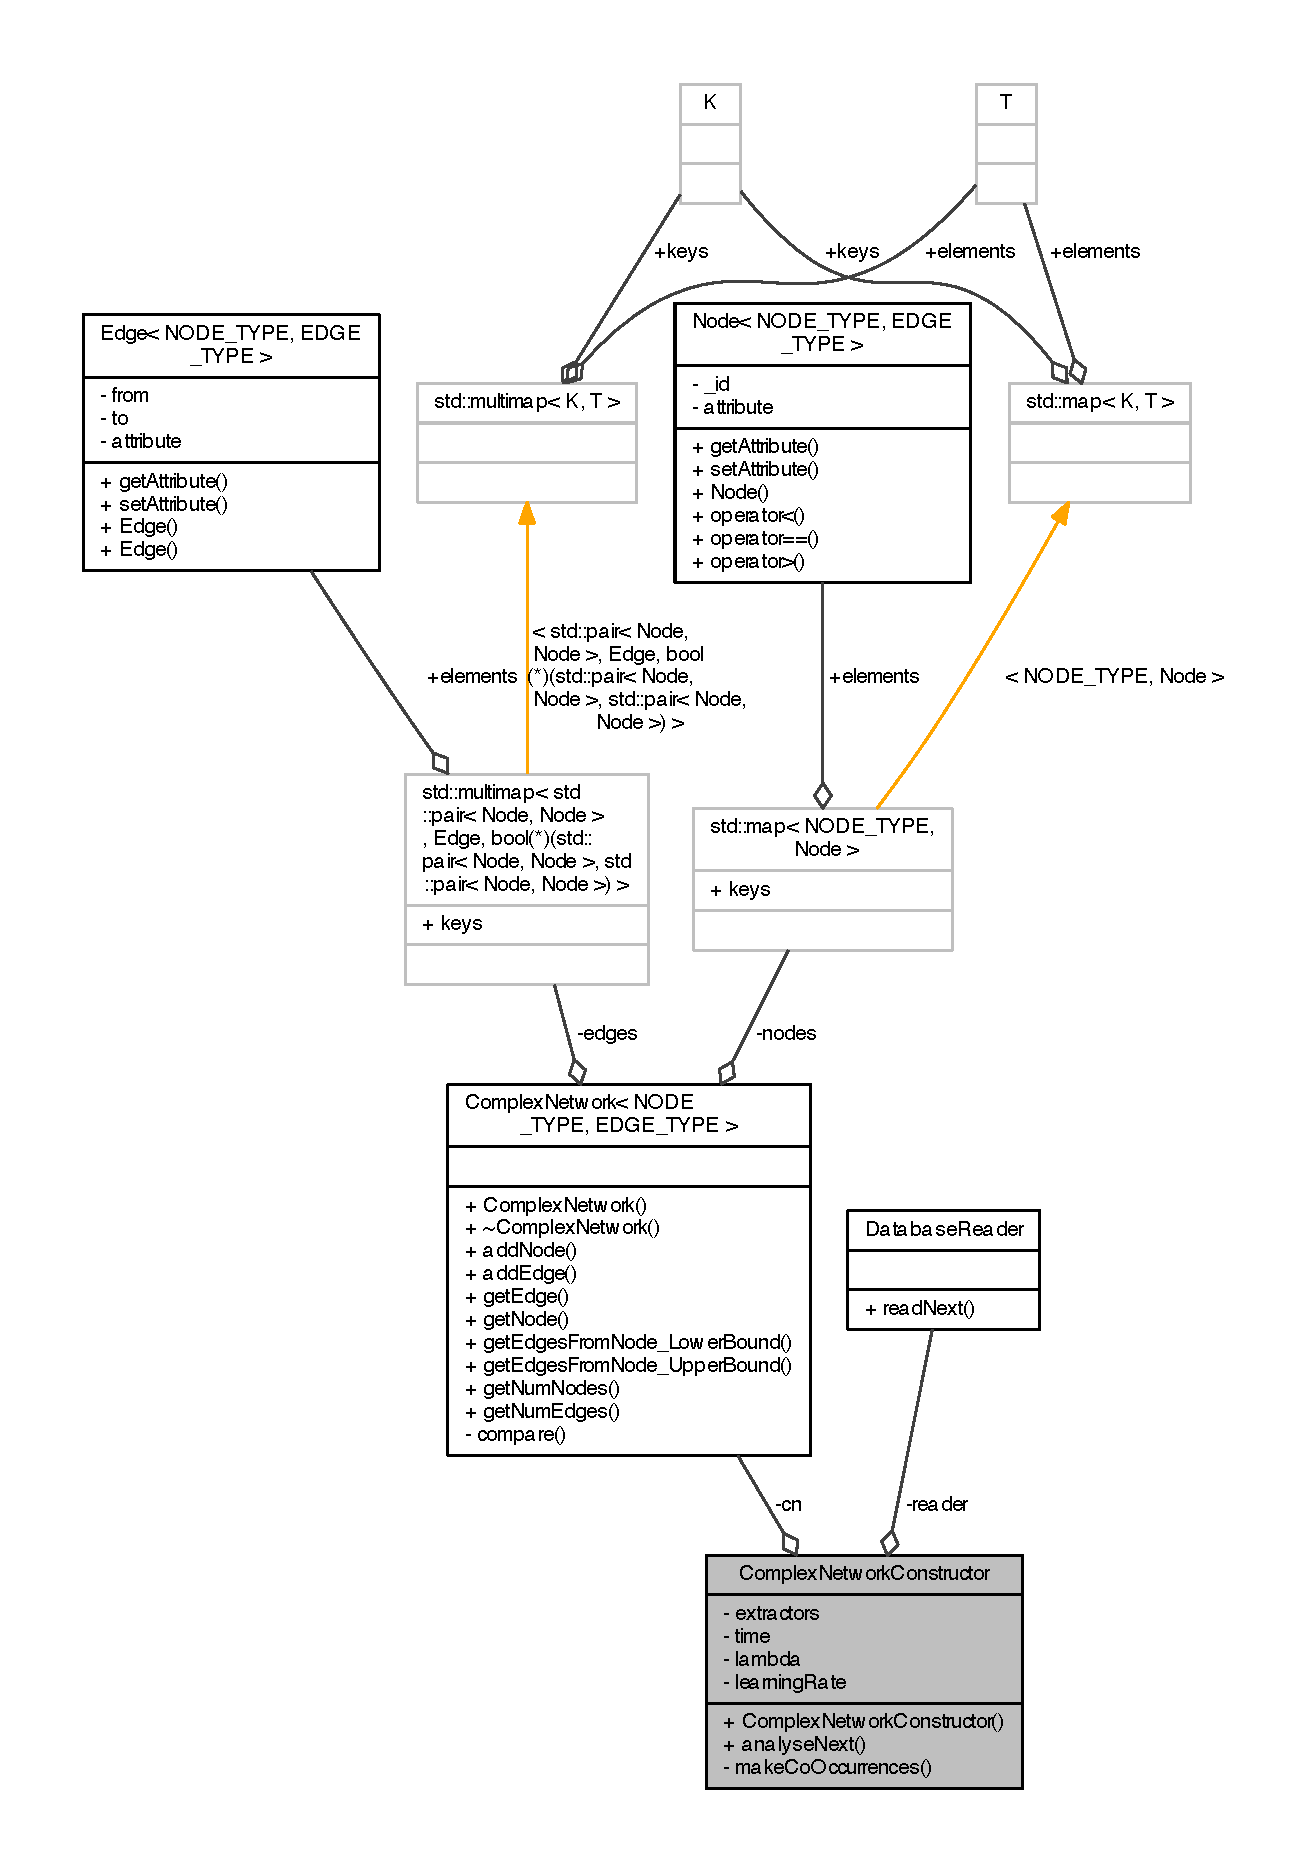
\includegraphics[width=350pt]{class_complex_network_constructor__coll__graph}
\end{center}
\end{figure}


\subsection{Constructor \& Destructor Documentation}
\hypertarget{class_complex_network_constructor_afe14ec2655225f646877381c87b86df3}{\index{Complex\+Network\+Constructor@{Complex\+Network\+Constructor}!Complex\+Network\+Constructor@{Complex\+Network\+Constructor}}
\index{Complex\+Network\+Constructor@{Complex\+Network\+Constructor}!Complex\+Network\+Constructor@{Complex\+Network\+Constructor}}
\subsubsection[{Complex\+Network\+Constructor}]{\setlength{\rightskip}{0pt plus 5cm}Complex\+Network\+Constructor\+::\+Complex\+Network\+Constructor (
\begin{DoxyParamCaption}
\item[{{\bf Features\+Complex\+Network} \&}]{cn, }
\item[{{\bf Database\+Reader} \&}]{reader, }
\item[{Q\+List$<$ {\bf Feature\+Factory\+Abstract} $\ast$ $>$}]{extractors}
\end{DoxyParamCaption}
)}}\label{class_complex_network_constructor_afe14ec2655225f646877381c87b86df3}


\subsection{Member Function Documentation}
\hypertarget{class_complex_network_constructor_a19d313488e2c19172e362b521f53e329}{\index{Complex\+Network\+Constructor@{Complex\+Network\+Constructor}!build@{build}}
\index{build@{build}!Complex\+Network\+Constructor@{Complex\+Network\+Constructor}}
\subsubsection[{build}]{\setlength{\rightskip}{0pt plus 5cm}void Complex\+Network\+Constructor\+::build (
\begin{DoxyParamCaption}
{}
\end{DoxyParamCaption}
)}}\label{class_complex_network_constructor_a19d313488e2c19172e362b521f53e329}


Here is the call graph for this function\+:\nopagebreak
\begin{figure}[H]
\begin{center}
\leavevmode
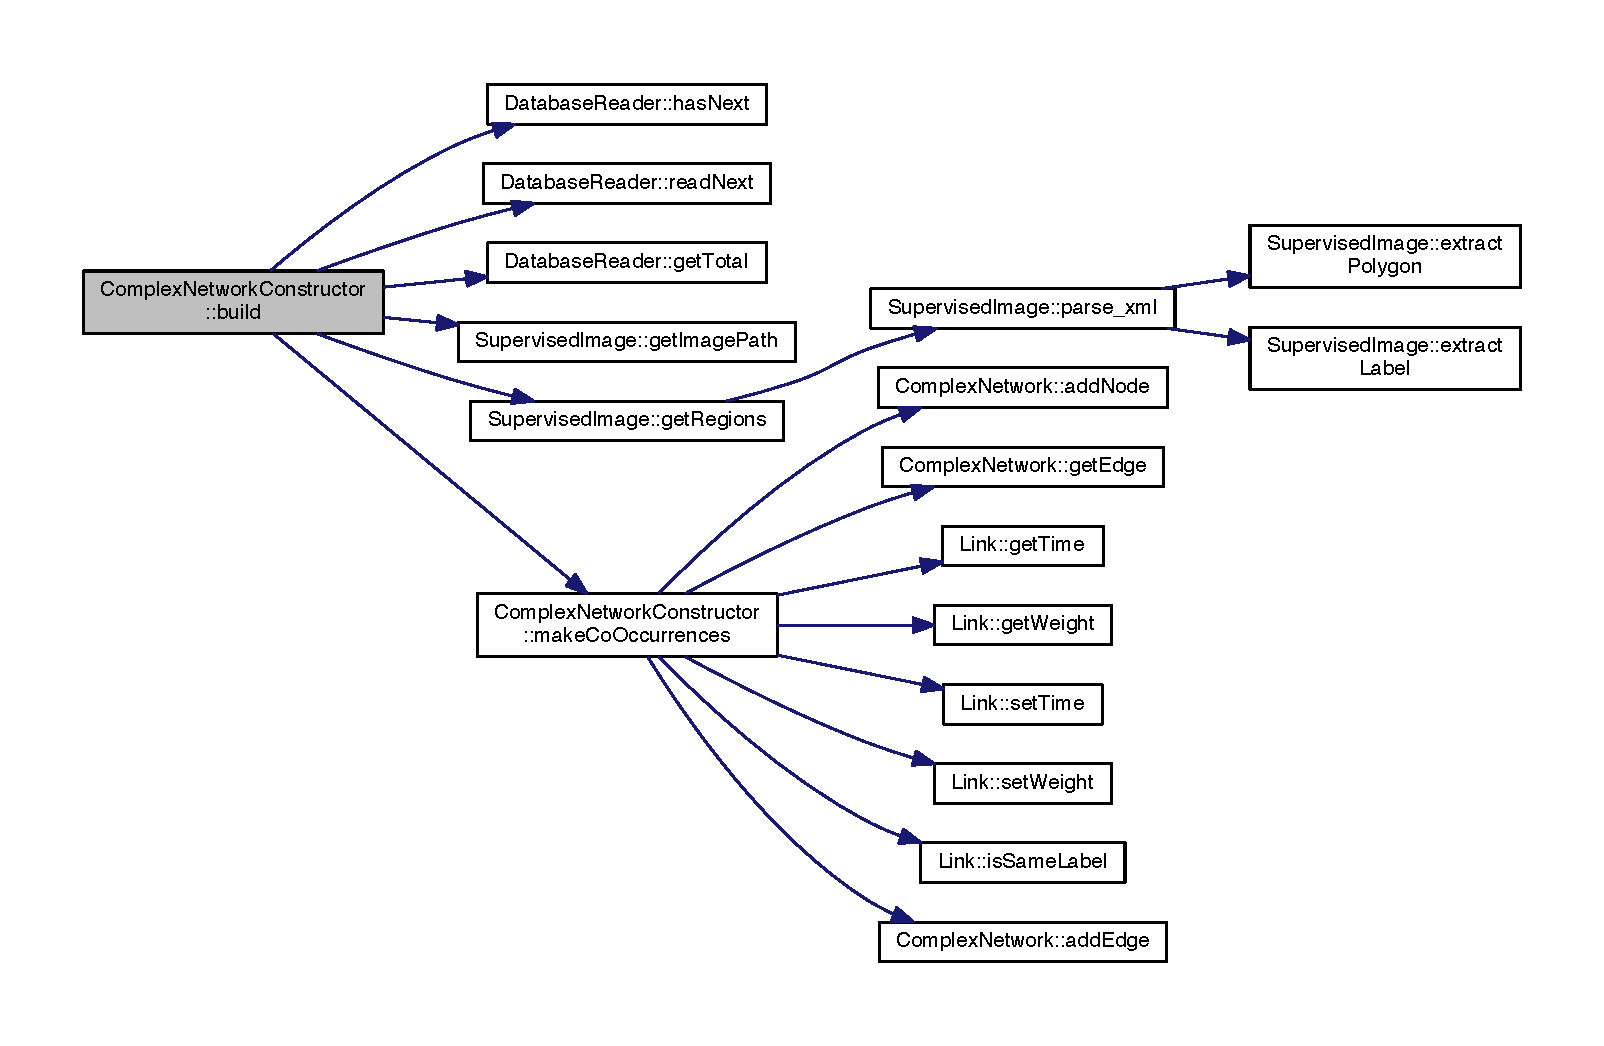
\includegraphics[width=350pt]{class_complex_network_constructor_a19d313488e2c19172e362b521f53e329_cgraph}
\end{center}
\end{figure}




Here is the caller graph for this function\+:
\nopagebreak
\begin{figure}[H]
\begin{center}
\leavevmode
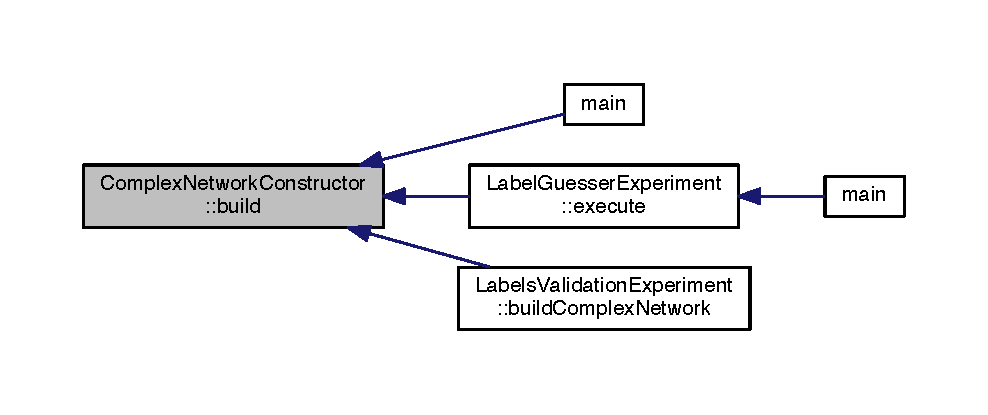
\includegraphics[width=350pt]{class_complex_network_constructor_a19d313488e2c19172e362b521f53e329_icgraph}
\end{center}
\end{figure}


\hypertarget{class_complex_network_constructor_aa41263b4bf0e157d451652d772f84ef7}{\index{Complex\+Network\+Constructor@{Complex\+Network\+Constructor}!make\+Co\+Occurrences@{make\+Co\+Occurrences}}
\index{make\+Co\+Occurrences@{make\+Co\+Occurrences}!Complex\+Network\+Constructor@{Complex\+Network\+Constructor}}
\subsubsection[{make\+Co\+Occurrences}]{\setlength{\rightskip}{0pt plus 5cm}void Complex\+Network\+Constructor\+::make\+Co\+Occurrences (
\begin{DoxyParamCaption}
\item[{Q\+Linked\+List$<$ {\bf Feature\+Abstract} $\ast$ $>$ \&}]{features, }
\item[{Q\+List$<$ int $>$ \&}]{regions\+Ids}
\end{DoxyParamCaption}
)\hspace{0.3cm}{\ttfamily [private]}}}\label{class_complex_network_constructor_aa41263b4bf0e157d451652d772f84ef7}
Atualiza os pesos as arestas de acordo com a Equação\+: \[ w_{i,j} = w_{i,j} + \alpha\left(\frac{\lambda}{\Delta t} - w_{i,j} \right) \] 

Here is the call graph for this function\+:\nopagebreak
\begin{figure}[H]
\begin{center}
\leavevmode
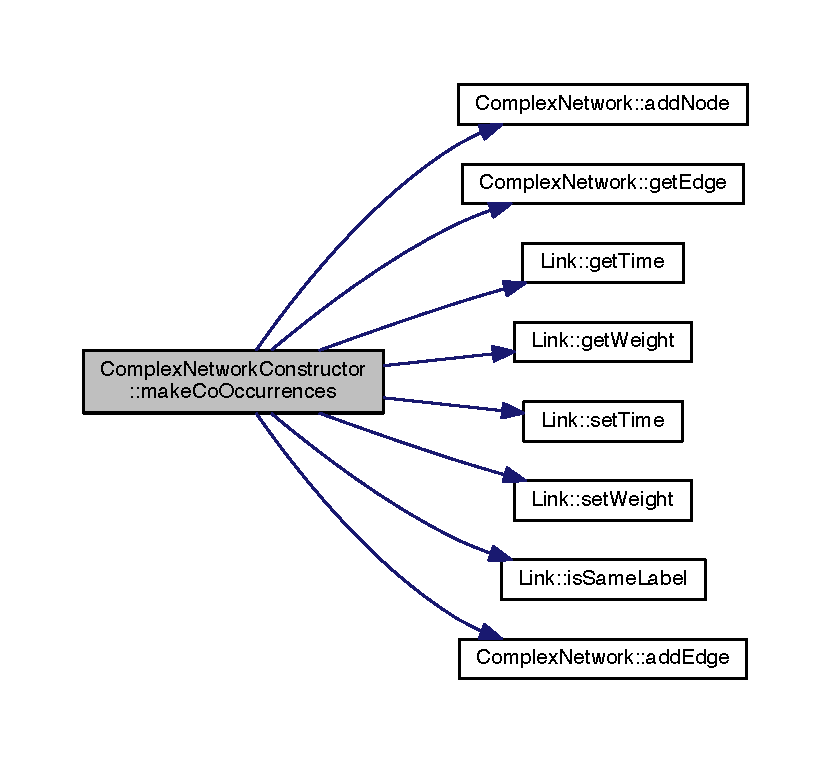
\includegraphics[width=350pt]{class_complex_network_constructor_aa41263b4bf0e157d451652d772f84ef7_cgraph}
\end{center}
\end{figure}




Here is the caller graph for this function\+:
\nopagebreak
\begin{figure}[H]
\begin{center}
\leavevmode
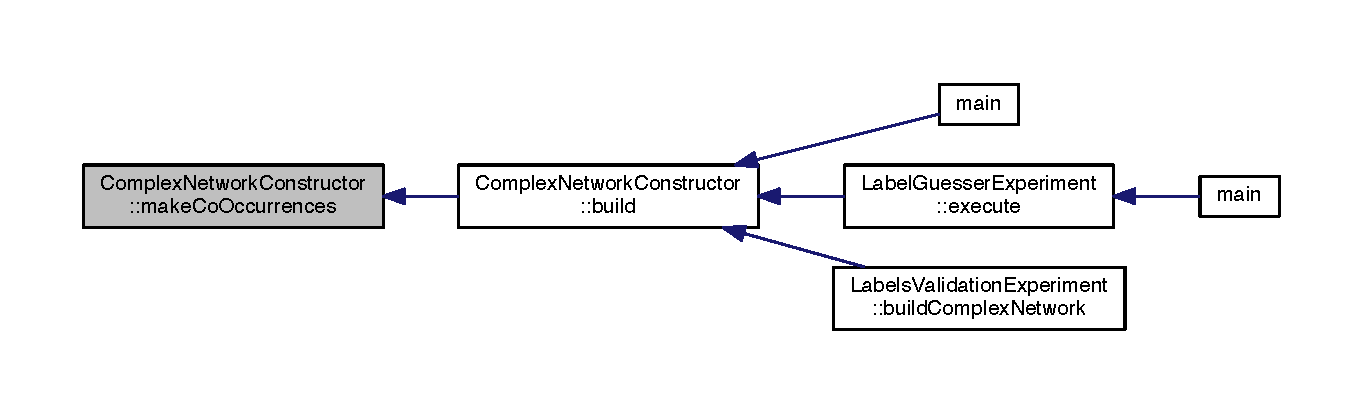
\includegraphics[width=350pt]{class_complex_network_constructor_aa41263b4bf0e157d451652d772f84ef7_icgraph}
\end{center}
\end{figure}


\hypertarget{class_complex_network_constructor_a8c4875120270d689a5fd08e47a6b4b59}{\index{Complex\+Network\+Constructor@{Complex\+Network\+Constructor}!recorrencia@{recorrencia}}
\index{recorrencia@{recorrencia}!Complex\+Network\+Constructor@{Complex\+Network\+Constructor}}
\subsubsection[{recorrencia}]{\setlength{\rightskip}{0pt plus 5cm}float Complex\+Network\+Constructor\+::recorrencia (
\begin{DoxyParamCaption}
\item[{float}]{time}
\end{DoxyParamCaption}
)\hspace{0.3cm}{\ttfamily [private]}}}\label{class_complex_network_constructor_a8c4875120270d689a5fd08e47a6b4b59}


\subsection{Member Data Documentation}
\hypertarget{class_complex_network_constructor_aa099456a58edc5c1885323061206b3e6}{\index{Complex\+Network\+Constructor@{Complex\+Network\+Constructor}!cn@{cn}}
\index{cn@{cn}!Complex\+Network\+Constructor@{Complex\+Network\+Constructor}}
\subsubsection[{cn}]{\setlength{\rightskip}{0pt plus 5cm}{\bf Features\+Complex\+Network}\& Complex\+Network\+Constructor\+::cn\hspace{0.3cm}{\ttfamily [private]}}}\label{class_complex_network_constructor_aa099456a58edc5c1885323061206b3e6}
\hypertarget{class_complex_network_constructor_ae79b538a8b9253cd71de5fef1be1c18a}{\index{Complex\+Network\+Constructor@{Complex\+Network\+Constructor}!extractors@{extractors}}
\index{extractors@{extractors}!Complex\+Network\+Constructor@{Complex\+Network\+Constructor}}
\subsubsection[{extractors}]{\setlength{\rightskip}{0pt plus 5cm}Q\+List$<${\bf Feature\+Factory\+Abstract}$\ast$$>$ Complex\+Network\+Constructor\+::extractors\hspace{0.3cm}{\ttfamily [private]}}}\label{class_complex_network_constructor_ae79b538a8b9253cd71de5fef1be1c18a}
\hypertarget{class_complex_network_constructor_ad616573ee07edff462c552d3fc2bfce7}{\index{Complex\+Network\+Constructor@{Complex\+Network\+Constructor}!index@{index}}
\index{index@{index}!Complex\+Network\+Constructor@{Complex\+Network\+Constructor}}
\subsubsection[{index}]{\setlength{\rightskip}{0pt plus 5cm}Q\+Hash$<${\bf Feature\+Abstract\+Key} , {\bf node\+\_\+id}$>$ Complex\+Network\+Constructor\+::index\hspace{0.3cm}{\ttfamily [private]}}}\label{class_complex_network_constructor_ad616573ee07edff462c552d3fc2bfce7}
\hypertarget{class_complex_network_constructor_a9d3e346719dc1f8f3093a48b8d44e669}{\index{Complex\+Network\+Constructor@{Complex\+Network\+Constructor}!lambda@{lambda}}
\index{lambda@{lambda}!Complex\+Network\+Constructor@{Complex\+Network\+Constructor}}
\subsubsection[{lambda}]{\setlength{\rightskip}{0pt plus 5cm}float Complex\+Network\+Constructor\+::lambda =80\hspace{0.3cm}{\ttfamily [private]}}}\label{class_complex_network_constructor_a9d3e346719dc1f8f3093a48b8d44e669}
Esta é a influência do tempo na aprendizagem $ \lambda $ \hypertarget{class_complex_network_constructor_aa7fe374b9733338b8176708f77d29c55}{\index{Complex\+Network\+Constructor@{Complex\+Network\+Constructor}!learning\+Rate@{learning\+Rate}}
\index{learning\+Rate@{learning\+Rate}!Complex\+Network\+Constructor@{Complex\+Network\+Constructor}}
\subsubsection[{learning\+Rate}]{\setlength{\rightskip}{0pt plus 5cm}float Complex\+Network\+Constructor\+::learning\+Rate =0.\+3\hspace{0.3cm}{\ttfamily [private]}}}\label{class_complex_network_constructor_aa7fe374b9733338b8176708f77d29c55}
Esta é a taxa de aprendizagem $ \alpha $ \hypertarget{class_complex_network_constructor_ad223ad7e464ff159d91a89deb4e943cc}{\index{Complex\+Network\+Constructor@{Complex\+Network\+Constructor}!reader@{reader}}
\index{reader@{reader}!Complex\+Network\+Constructor@{Complex\+Network\+Constructor}}
\subsubsection[{reader}]{\setlength{\rightskip}{0pt plus 5cm}{\bf Database\+Reader}\& Complex\+Network\+Constructor\+::reader\hspace{0.3cm}{\ttfamily [private]}}}\label{class_complex_network_constructor_ad223ad7e464ff159d91a89deb4e943cc}
\hypertarget{class_complex_network_constructor_afc016404ca7dda4b05807e3ca004c308}{\index{Complex\+Network\+Constructor@{Complex\+Network\+Constructor}!time@{time}}
\index{time@{time}!Complex\+Network\+Constructor@{Complex\+Network\+Constructor}}
\subsubsection[{time}]{\setlength{\rightskip}{0pt plus 5cm}unsigned long long int Complex\+Network\+Constructor\+::time =1\hspace{0.3cm}{\ttfamily [private]}}}\label{class_complex_network_constructor_afc016404ca7dda4b05807e3ca004c308}


The documentation for this class was generated from the following files\+:\begin{DoxyCompactItemize}
\item 
Sources/\+Utilities/\hyperlink{_complex_network_constructor_8hpp}{Complex\+Network\+Constructor.\+hpp}\item 
Sources/\+Utilities/\hyperlink{_complex_network_constructor_8cpp}{Complex\+Network\+Constructor.\+cpp}\end{DoxyCompactItemize}

\hypertarget{class_database_reader}{\section{Database\+Reader Class Reference}
\label{class_database_reader}\index{Database\+Reader@{Database\+Reader}}
}


{\ttfamily \#include $<$Database\+Reader.\+hpp$>$}



Inheritance diagram for Database\+Reader\+:
\nopagebreak
\begin{figure}[H]
\begin{center}
\leavevmode
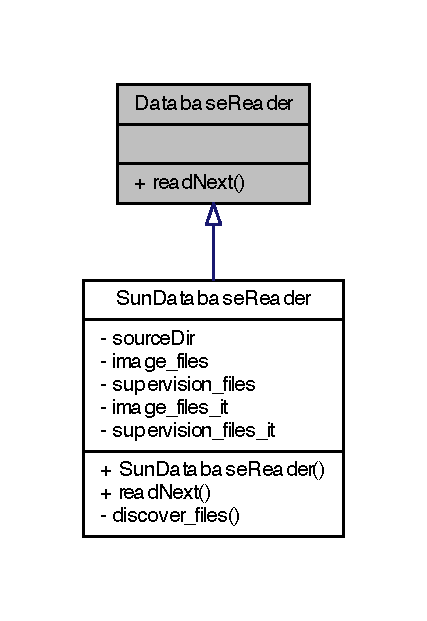
\includegraphics[width=205pt]{class_database_reader__inherit__graph}
\end{center}
\end{figure}


Collaboration diagram for Database\+Reader\+:
\nopagebreak
\begin{figure}[H]
\begin{center}
\leavevmode
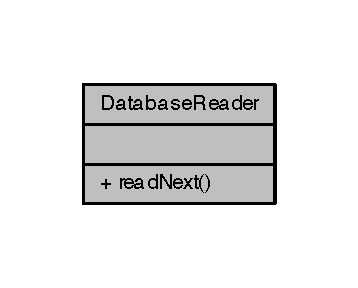
\includegraphics[width=172pt]{class_database_reader__coll__graph}
\end{center}
\end{figure}
\subsection*{Public Member Functions}
\begin{DoxyCompactItemize}
\item 
virtual \hyperlink{class_supervised_image}{Supervised\+Image} $\ast$ \hyperlink{class_database_reader_ae6a76cba6f3d4dad64b70b59c701b9f6}{read\+Next} ()=0
\end{DoxyCompactItemize}


\subsection{Member Function Documentation}
\hypertarget{class_database_reader_ae6a76cba6f3d4dad64b70b59c701b9f6}{\index{Database\+Reader@{Database\+Reader}!read\+Next@{read\+Next}}
\index{read\+Next@{read\+Next}!Database\+Reader@{Database\+Reader}}
\subsubsection[{read\+Next}]{\setlength{\rightskip}{0pt plus 5cm}virtual {\bf Supervised\+Image}$\ast$ Database\+Reader\+::read\+Next (
\begin{DoxyParamCaption}
{}
\end{DoxyParamCaption}
)\hspace{0.3cm}{\ttfamily [pure virtual]}}}\label{class_database_reader_ae6a76cba6f3d4dad64b70b59c701b9f6}


Implemented in \hyperlink{class_sun_database_reader_aadf059f614225be059e05a7c3a75fb26}{Sun\+Database\+Reader}.



The documentation for this class was generated from the following file\+:\begin{DoxyCompactItemize}
\item 
src/\hyperlink{_database_reader_8hpp}{Database\+Reader.\+hpp}\end{DoxyCompactItemize}

\hypertarget{class_edge}{\section{Edge$<$ N\+O\+D\+E\+\_\+\+T\+Y\+P\+E, E\+D\+G\+E\+\_\+\+T\+Y\+P\+E $>$ Class Template Reference}
\label{class_edge}\index{Edge$<$ N\+O\+D\+E\+\_\+\+T\+Y\+P\+E, E\+D\+G\+E\+\_\+\+T\+Y\+P\+E $>$@{Edge$<$ N\+O\+D\+E\+\_\+\+T\+Y\+P\+E, E\+D\+G\+E\+\_\+\+T\+Y\+P\+E $>$}}
}


{\ttfamily \#include $<$Edge.\+hpp$>$}

\subsection*{Public Member Functions}
\begin{DoxyCompactItemize}
\item 
E\+D\+G\+E\+\_\+\+T\+Y\+P\+E \hyperlink{class_edge_a3352ae81439c772a0ebe640f14f8b910}{get\+Attribute} ()
\item 
void \hyperlink{class_edge_aa63f7fac23602924d2e19f1389a93620}{set\+Attribute} (E\+D\+G\+E\+\_\+\+T\+Y\+P\+E attr)
\item 
\hyperlink{class_edge_a16c5157732e48a737ca0a1d7841e8e19}{Edge} (\hyperlink{class_node}{Node}$<$ N\+O\+D\+E\+\_\+\+T\+Y\+P\+E, E\+D\+G\+E\+\_\+\+T\+Y\+P\+E $>$ $\ast$\hyperlink{class_edge_a1bffa41df2941b7d55c59a5031f78e14}{from}, \hyperlink{class_node}{Node}$<$ N\+O\+D\+E\+\_\+\+T\+Y\+P\+E, E\+D\+G\+E\+\_\+\+T\+Y\+P\+E $>$ $\ast$\hyperlink{class_edge_a7ba6dee1554e4a0a7cf69862e90fdd85}{to})
\item 
\hyperlink{class_edge_a6d1f57f17db61020c1e51c09ff8ab7bb}{Edge} (\hyperlink{class_node}{Node}$<$ N\+O\+D\+E\+\_\+\+T\+Y\+P\+E, E\+D\+G\+E\+\_\+\+T\+Y\+P\+E $>$ $\ast$\hyperlink{class_edge_a1bffa41df2941b7d55c59a5031f78e14}{from}, \hyperlink{class_node}{Node}$<$ N\+O\+D\+E\+\_\+\+T\+Y\+P\+E, E\+D\+G\+E\+\_\+\+T\+Y\+P\+E $>$ $\ast$\hyperlink{class_edge_a7ba6dee1554e4a0a7cf69862e90fdd85}{to}, E\+D\+G\+E\+\_\+\+T\+Y\+P\+E \hyperlink{class_edge_ae49cc056dfa848b0a1beef821d81a31d}{attribute})
\end{DoxyCompactItemize}
\subsection*{Private Attributes}
\begin{DoxyCompactItemize}
\item 
\hyperlink{class_node}{Node}$<$ N\+O\+D\+E\+\_\+\+T\+Y\+P\+E, E\+D\+G\+E\+\_\+\+T\+Y\+P\+E $>$ $\ast$ \hyperlink{class_edge_a1bffa41df2941b7d55c59a5031f78e14}{from}
\item 
\hyperlink{class_node}{Node}$<$ N\+O\+D\+E\+\_\+\+T\+Y\+P\+E, E\+D\+G\+E\+\_\+\+T\+Y\+P\+E $>$ $\ast$ \hyperlink{class_edge_a7ba6dee1554e4a0a7cf69862e90fdd85}{to}
\item 
E\+D\+G\+E\+\_\+\+T\+Y\+P\+E \hyperlink{class_edge_ae49cc056dfa848b0a1beef821d81a31d}{attribute}
\end{DoxyCompactItemize}
\subsection*{Friends}
\begin{DoxyCompactItemize}
\item 
class \hyperlink{class_edge_ad8438fc5199b628ea294f77319026b6a}{Complex\+Network$<$ N\+O\+D\+E\+\_\+\+T\+Y\+P\+E, E\+D\+G\+E\+\_\+\+T\+Y\+P\+E $>$}
\end{DoxyCompactItemize}


Collaboration diagram for Edge$<$ N\+O\+D\+E\+\_\+\+T\+Y\+P\+E, E\+D\+G\+E\+\_\+\+T\+Y\+P\+E $>$\+:\nopagebreak
\begin{figure}[H]
\begin{center}
\leavevmode
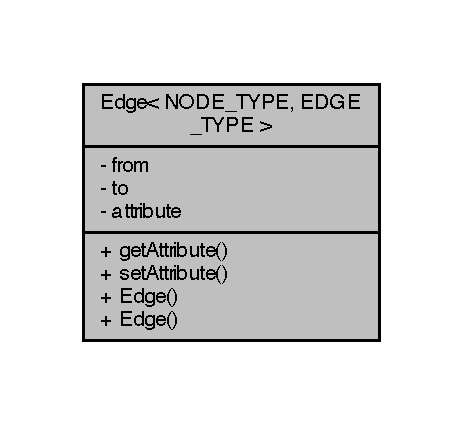
\includegraphics[width=222pt]{class_edge__coll__graph}
\end{center}
\end{figure}


\subsection{Constructor \& Destructor Documentation}
\hypertarget{class_edge_a16c5157732e48a737ca0a1d7841e8e19}{\index{Edge@{Edge}!Edge@{Edge}}
\index{Edge@{Edge}!Edge@{Edge}}
\subsubsection[{Edge}]{\setlength{\rightskip}{0pt plus 5cm}template$<$class N\+O\+D\+E\+\_\+\+T\+Y\+P\+E , class E\+D\+G\+E\+\_\+\+T\+Y\+P\+E $>$ {\bf Edge}$<$ N\+O\+D\+E\+\_\+\+T\+Y\+P\+E, E\+D\+G\+E\+\_\+\+T\+Y\+P\+E $>$\+::{\bf Edge} (
\begin{DoxyParamCaption}
\item[{{\bf Node}$<$ N\+O\+D\+E\+\_\+\+T\+Y\+P\+E, E\+D\+G\+E\+\_\+\+T\+Y\+P\+E $>$ $\ast$}]{from, }
\item[{{\bf Node}$<$ N\+O\+D\+E\+\_\+\+T\+Y\+P\+E, E\+D\+G\+E\+\_\+\+T\+Y\+P\+E $>$ $\ast$}]{to}
\end{DoxyParamCaption}
)}}\label{class_edge_a16c5157732e48a737ca0a1d7841e8e19}
Por padrão as arestas são direcionadas 
\begin{DoxyParams}{Parameters}
{\em from} & Nó de saída \\
\hline
{\em to} & Nó de entrada \\
\hline
\end{DoxyParams}
\hypertarget{class_edge_a6d1f57f17db61020c1e51c09ff8ab7bb}{\index{Edge@{Edge}!Edge@{Edge}}
\index{Edge@{Edge}!Edge@{Edge}}
\subsubsection[{Edge}]{\setlength{\rightskip}{0pt plus 5cm}template$<$class N\+O\+D\+E\+\_\+\+T\+Y\+P\+E , class E\+D\+G\+E\+\_\+\+T\+Y\+P\+E $>$ {\bf Edge}$<$ N\+O\+D\+E\+\_\+\+T\+Y\+P\+E, E\+D\+G\+E\+\_\+\+T\+Y\+P\+E $>$\+::{\bf Edge} (
\begin{DoxyParamCaption}
\item[{{\bf Node}$<$ N\+O\+D\+E\+\_\+\+T\+Y\+P\+E, E\+D\+G\+E\+\_\+\+T\+Y\+P\+E $>$ $\ast$}]{from, }
\item[{{\bf Node}$<$ N\+O\+D\+E\+\_\+\+T\+Y\+P\+E, E\+D\+G\+E\+\_\+\+T\+Y\+P\+E $>$ $\ast$}]{to, }
\item[{E\+D\+G\+E\+\_\+\+T\+Y\+P\+E}]{attribute}
\end{DoxyParamCaption}
)}}\label{class_edge_a6d1f57f17db61020c1e51c09ff8ab7bb}
Por padrão as arestas são direcionadas 
\begin{DoxyParams}{Parameters}
{\em from} & Nó de saída \\
\hline
{\em to} & Nó de entrada \\
\hline
{\em attribute} & Atributo da aresta \\
\hline
\end{DoxyParams}


\subsection{Member Function Documentation}
\hypertarget{class_edge_a3352ae81439c772a0ebe640f14f8b910}{\index{Edge@{Edge}!get\+Attribute@{get\+Attribute}}
\index{get\+Attribute@{get\+Attribute}!Edge@{Edge}}
\subsubsection[{get\+Attribute}]{\setlength{\rightskip}{0pt plus 5cm}template$<$class N\+O\+D\+E\+\_\+\+T\+Y\+P\+E , class E\+D\+G\+E\+\_\+\+T\+Y\+P\+E $>$ E\+D\+G\+E\+\_\+\+T\+Y\+P\+E {\bf Edge}$<$ N\+O\+D\+E\+\_\+\+T\+Y\+P\+E, E\+D\+G\+E\+\_\+\+T\+Y\+P\+E $>$\+::get\+Attribute (
\begin{DoxyParamCaption}
{}
\end{DoxyParamCaption}
)}}\label{class_edge_a3352ae81439c772a0ebe640f14f8b910}


Here is the caller graph for this function\+:\nopagebreak
\begin{figure}[H]
\begin{center}
\leavevmode
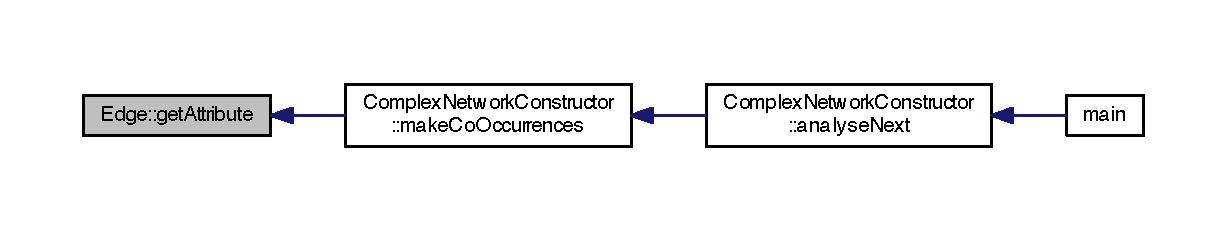
\includegraphics[width=350pt]{class_edge_a3352ae81439c772a0ebe640f14f8b910_icgraph}
\end{center}
\end{figure}


\hypertarget{class_edge_aa63f7fac23602924d2e19f1389a93620}{\index{Edge@{Edge}!set\+Attribute@{set\+Attribute}}
\index{set\+Attribute@{set\+Attribute}!Edge@{Edge}}
\subsubsection[{set\+Attribute}]{\setlength{\rightskip}{0pt plus 5cm}template$<$class N\+O\+D\+E\+\_\+\+T\+Y\+P\+E , class E\+D\+G\+E\+\_\+\+T\+Y\+P\+E $>$ void {\bf Edge}$<$ N\+O\+D\+E\+\_\+\+T\+Y\+P\+E, E\+D\+G\+E\+\_\+\+T\+Y\+P\+E $>$\+::set\+Attribute (
\begin{DoxyParamCaption}
\item[{E\+D\+G\+E\+\_\+\+T\+Y\+P\+E}]{attr}
\end{DoxyParamCaption}
)}}\label{class_edge_aa63f7fac23602924d2e19f1389a93620}


Here is the caller graph for this function\+:\nopagebreak
\begin{figure}[H]
\begin{center}
\leavevmode
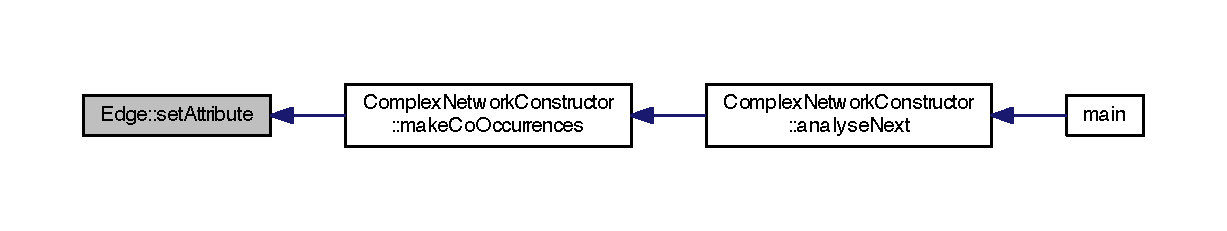
\includegraphics[width=350pt]{class_edge_aa63f7fac23602924d2e19f1389a93620_icgraph}
\end{center}
\end{figure}




\subsection{Friends And Related Function Documentation}
\hypertarget{class_edge_ad8438fc5199b628ea294f77319026b6a}{\index{Edge@{Edge}!Complex\+Network$<$ N\+O\+D\+E\+\_\+\+T\+Y\+P\+E, E\+D\+G\+E\+\_\+\+T\+Y\+P\+E $>$@{Complex\+Network$<$ N\+O\+D\+E\+\_\+\+T\+Y\+P\+E, E\+D\+G\+E\+\_\+\+T\+Y\+P\+E $>$}}
\index{Complex\+Network$<$ N\+O\+D\+E\+\_\+\+T\+Y\+P\+E, E\+D\+G\+E\+\_\+\+T\+Y\+P\+E $>$@{Complex\+Network$<$ N\+O\+D\+E\+\_\+\+T\+Y\+P\+E, E\+D\+G\+E\+\_\+\+T\+Y\+P\+E $>$}!Edge@{Edge}}
\subsubsection[{Complex\+Network$<$ N\+O\+D\+E\+\_\+\+T\+Y\+P\+E, E\+D\+G\+E\+\_\+\+T\+Y\+P\+E $>$}]{\setlength{\rightskip}{0pt plus 5cm}template$<$class N\+O\+D\+E\+\_\+\+T\+Y\+P\+E, class E\+D\+G\+E\+\_\+\+T\+Y\+P\+E$>$ friend class {\bf Complex\+Network}$<$ N\+O\+D\+E\+\_\+\+T\+Y\+P\+E, E\+D\+G\+E\+\_\+\+T\+Y\+P\+E $>$\hspace{0.3cm}{\ttfamily [friend]}}}\label{class_edge_ad8438fc5199b628ea294f77319026b6a}


\subsection{Member Data Documentation}
\hypertarget{class_edge_ae49cc056dfa848b0a1beef821d81a31d}{\index{Edge@{Edge}!attribute@{attribute}}
\index{attribute@{attribute}!Edge@{Edge}}
\subsubsection[{attribute}]{\setlength{\rightskip}{0pt plus 5cm}template$<$class N\+O\+D\+E\+\_\+\+T\+Y\+P\+E, class E\+D\+G\+E\+\_\+\+T\+Y\+P\+E$>$ E\+D\+G\+E\+\_\+\+T\+Y\+P\+E {\bf Edge}$<$ N\+O\+D\+E\+\_\+\+T\+Y\+P\+E, E\+D\+G\+E\+\_\+\+T\+Y\+P\+E $>$\+::attribute\hspace{0.3cm}{\ttfamily [private]}}}\label{class_edge_ae49cc056dfa848b0a1beef821d81a31d}
\hypertarget{class_edge_a1bffa41df2941b7d55c59a5031f78e14}{\index{Edge@{Edge}!from@{from}}
\index{from@{from}!Edge@{Edge}}
\subsubsection[{from}]{\setlength{\rightskip}{0pt plus 5cm}template$<$class N\+O\+D\+E\+\_\+\+T\+Y\+P\+E, class E\+D\+G\+E\+\_\+\+T\+Y\+P\+E$>$ {\bf Node}$<$N\+O\+D\+E\+\_\+\+T\+Y\+P\+E, E\+D\+G\+E\+\_\+\+T\+Y\+P\+E$>$$\ast$ {\bf Edge}$<$ N\+O\+D\+E\+\_\+\+T\+Y\+P\+E, E\+D\+G\+E\+\_\+\+T\+Y\+P\+E $>$\+::from\hspace{0.3cm}{\ttfamily [private]}}}\label{class_edge_a1bffa41df2941b7d55c59a5031f78e14}
\hypertarget{class_edge_a7ba6dee1554e4a0a7cf69862e90fdd85}{\index{Edge@{Edge}!to@{to}}
\index{to@{to}!Edge@{Edge}}
\subsubsection[{to}]{\setlength{\rightskip}{0pt plus 5cm}template$<$class N\+O\+D\+E\+\_\+\+T\+Y\+P\+E, class E\+D\+G\+E\+\_\+\+T\+Y\+P\+E$>$ {\bf Node}$<$N\+O\+D\+E\+\_\+\+T\+Y\+P\+E, E\+D\+G\+E\+\_\+\+T\+Y\+P\+E$>$$\ast$ {\bf Edge}$<$ N\+O\+D\+E\+\_\+\+T\+Y\+P\+E, E\+D\+G\+E\+\_\+\+T\+Y\+P\+E $>$\+::to\hspace{0.3cm}{\ttfamily [private]}}}\label{class_edge_a7ba6dee1554e4a0a7cf69862e90fdd85}


The documentation for this class was generated from the following file\+:\begin{DoxyCompactItemize}
\item 
src/\hyperlink{_edge_8hpp}{Edge.\+hpp}\end{DoxyCompactItemize}

\hypertarget{class_feature}{\section{Feature Class Reference}
\label{class_feature}\index{Feature@{Feature}}
}


{\ttfamily \#include $<$Feature.\+hpp$>$}



Inheritance diagram for Feature\+:
\nopagebreak
\begin{figure}[H]
\begin{center}
\leavevmode
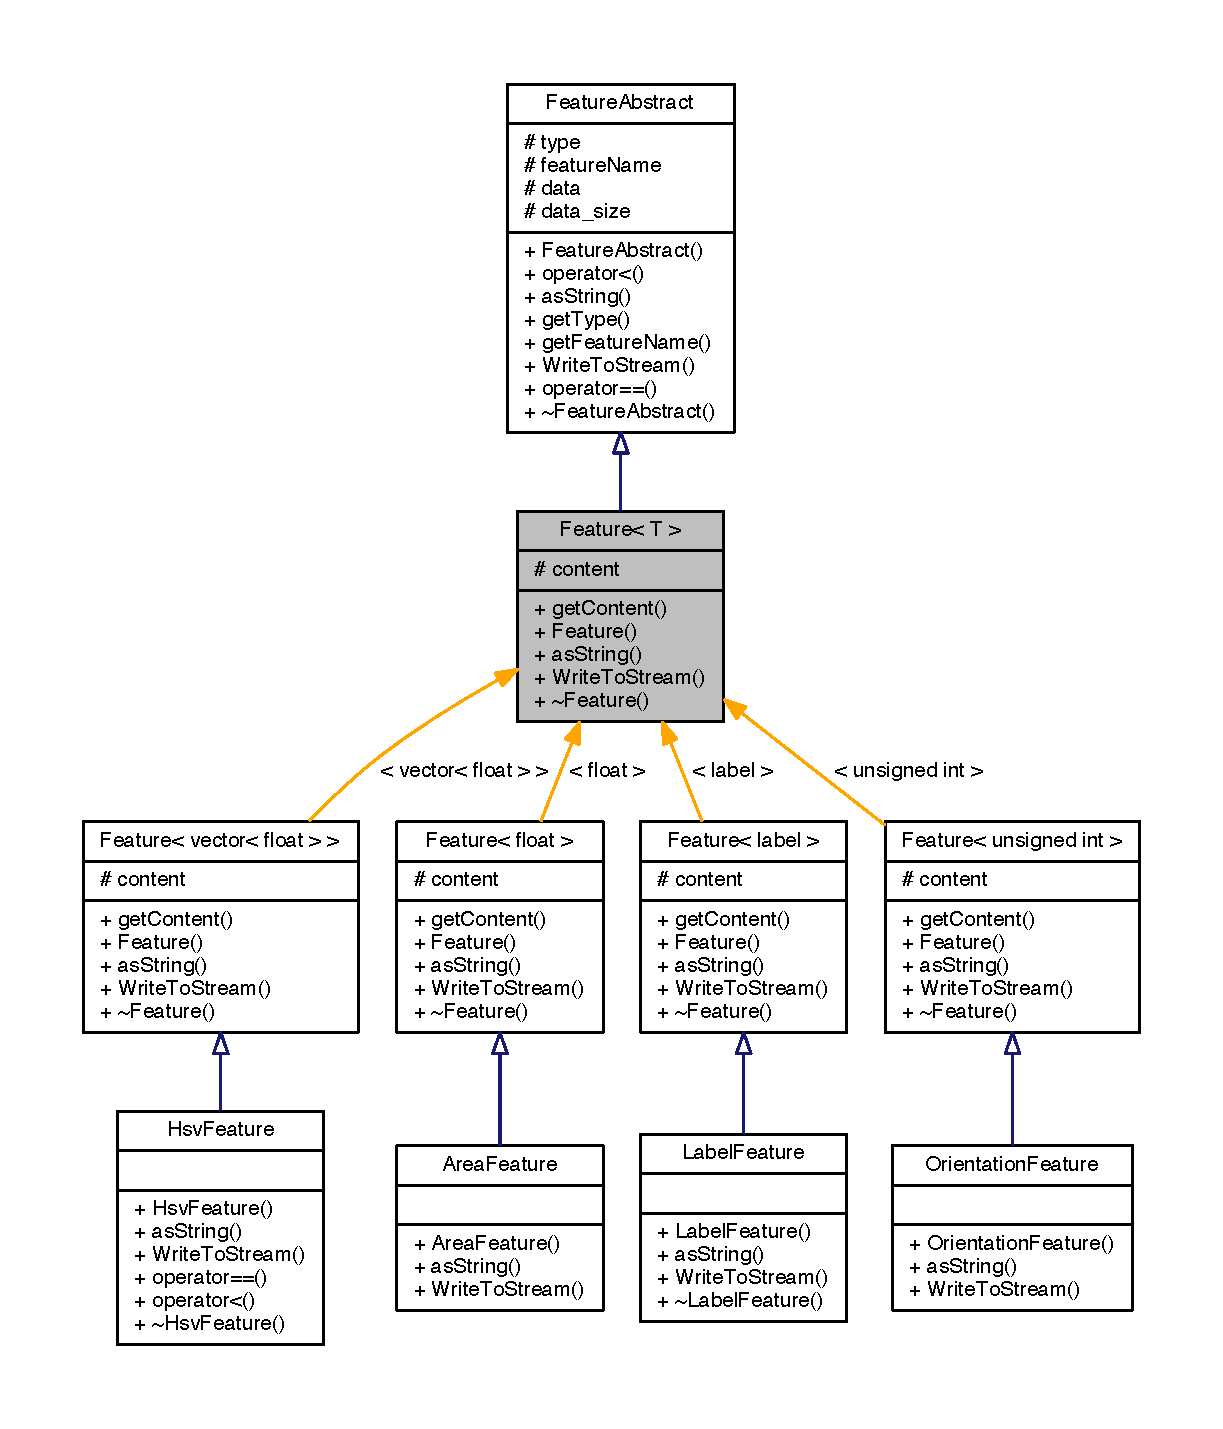
\includegraphics[width=171pt]{class_feature__inherit__graph}
\end{center}
\end{figure}


Collaboration diagram for Feature\+:
\nopagebreak
\begin{figure}[H]
\begin{center}
\leavevmode
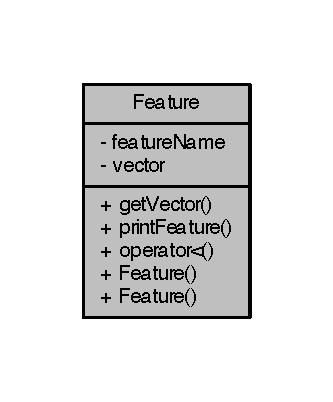
\includegraphics[width=185pt]{class_feature__coll__graph}
\end{center}
\end{figure}
\subsection*{Public Member Functions}
\begin{DoxyCompactItemize}
\item 
const Q\+Vector$<$ float $>$ \& \hyperlink{class_feature_ab96106b9d1ba89cfa00ffb63a26b2130}{get\+Vector} () const 
\item 
virtual void \hyperlink{class_feature_a6ce2b27ca0932c42b99c41c3d1d20366}{extract\+Feature} ()=0
\item 
void \hyperlink{class_feature_a0e73c5cb157120a30704efb4af866ec0}{print\+Feature} () const 
\end{DoxyCompactItemize}
\subsection*{Protected Member Functions}
\begin{DoxyCompactItemize}
\item 
\hyperlink{class_feature_a4129c864c4c97078084332515f6f20d1}{Feature} (\hyperlink{class_region}{Region} $\ast$\hyperlink{class_feature_a134c6b5022108c2a1000c7c88c40f352}{region})
\end{DoxyCompactItemize}
\subsection*{Protected Attributes}
\begin{DoxyCompactItemize}
\item 
\hyperlink{class_region}{Region} $\ast$ \hyperlink{class_feature_a134c6b5022108c2a1000c7c88c40f352}{region}
\item 
Q\+Vector$<$ float $>$ \hyperlink{class_feature_a8158dfca752942aeb84f35c363184d95}{vector}
\end{DoxyCompactItemize}


\subsection{Constructor \& Destructor Documentation}
\hypertarget{class_feature_a4129c864c4c97078084332515f6f20d1}{\index{Feature@{Feature}!Feature@{Feature}}
\index{Feature@{Feature}!Feature@{Feature}}
\subsubsection[{Feature}]{\setlength{\rightskip}{0pt plus 5cm}Feature\+::\+Feature (
\begin{DoxyParamCaption}
\item[{{\bf Region} $\ast$}]{region}
\end{DoxyParamCaption}
)\hspace{0.3cm}{\ttfamily [protected]}}}\label{class_feature_a4129c864c4c97078084332515f6f20d1}


\subsection{Member Function Documentation}
\hypertarget{class_feature_a6ce2b27ca0932c42b99c41c3d1d20366}{\index{Feature@{Feature}!extract\+Feature@{extract\+Feature}}
\index{extract\+Feature@{extract\+Feature}!Feature@{Feature}}
\subsubsection[{extract\+Feature}]{\setlength{\rightskip}{0pt plus 5cm}virtual void Feature\+::extract\+Feature (
\begin{DoxyParamCaption}
{}
\end{DoxyParamCaption}
)\hspace{0.3cm}{\ttfamily [pure virtual]}}}\label{class_feature_a6ce2b27ca0932c42b99c41c3d1d20366}


Implemented in \hyperlink{class_area_feature_a076f7a3918e7aa54e64b7e45733ad63d}{Area\+Feature}.

\hypertarget{class_feature_ab96106b9d1ba89cfa00ffb63a26b2130}{\index{Feature@{Feature}!get\+Vector@{get\+Vector}}
\index{get\+Vector@{get\+Vector}!Feature@{Feature}}
\subsubsection[{get\+Vector}]{\setlength{\rightskip}{0pt plus 5cm}const Q\+Vector$<$ float $>$ \& Feature\+::get\+Vector (
\begin{DoxyParamCaption}
{}
\end{DoxyParamCaption}
) const}}\label{class_feature_ab96106b9d1ba89cfa00ffb63a26b2130}
\hypertarget{class_feature_a0e73c5cb157120a30704efb4af866ec0}{\index{Feature@{Feature}!print\+Feature@{print\+Feature}}
\index{print\+Feature@{print\+Feature}!Feature@{Feature}}
\subsubsection[{print\+Feature}]{\setlength{\rightskip}{0pt plus 5cm}void Feature\+::print\+Feature (
\begin{DoxyParamCaption}
{}
\end{DoxyParamCaption}
) const}}\label{class_feature_a0e73c5cb157120a30704efb4af866ec0}


Here is the caller graph for this function\+:
\nopagebreak
\begin{figure}[H]
\begin{center}
\leavevmode
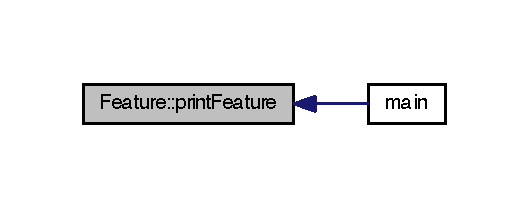
\includegraphics[width=254pt]{class_feature_a0e73c5cb157120a30704efb4af866ec0_icgraph}
\end{center}
\end{figure}




\subsection{Member Data Documentation}
\hypertarget{class_feature_a134c6b5022108c2a1000c7c88c40f352}{\index{Feature@{Feature}!region@{region}}
\index{region@{region}!Feature@{Feature}}
\subsubsection[{region}]{\setlength{\rightskip}{0pt plus 5cm}{\bf Region}$\ast$ Feature\+::region\hspace{0.3cm}{\ttfamily [protected]}}}\label{class_feature_a134c6b5022108c2a1000c7c88c40f352}
\hypertarget{class_feature_a8158dfca752942aeb84f35c363184d95}{\index{Feature@{Feature}!vector@{vector}}
\index{vector@{vector}!Feature@{Feature}}
\subsubsection[{vector}]{\setlength{\rightskip}{0pt plus 5cm}Q\+Vector$<$float$>$ Feature\+::vector\hspace{0.3cm}{\ttfamily [protected]}}}\label{class_feature_a8158dfca752942aeb84f35c363184d95}


The documentation for this class was generated from the following files\+:\begin{DoxyCompactItemize}
\item 
src/\hyperlink{_feature_8hpp}{Feature.\+hpp}\item 
src/\hyperlink{_feature_8cpp}{Feature.\+cpp}\end{DoxyCompactItemize}

\hypertarget{class_feature_extractor}{\section{Feature\+Extractor Class Reference}
\label{class_feature_extractor}\index{Feature\+Extractor@{Feature\+Extractor}}
}


{\ttfamily \#include $<$Feature\+Extractor.\+hpp$>$}



Inheritance diagram for Feature\+Extractor\+:
\nopagebreak
\begin{figure}[H]
\begin{center}
\leavevmode
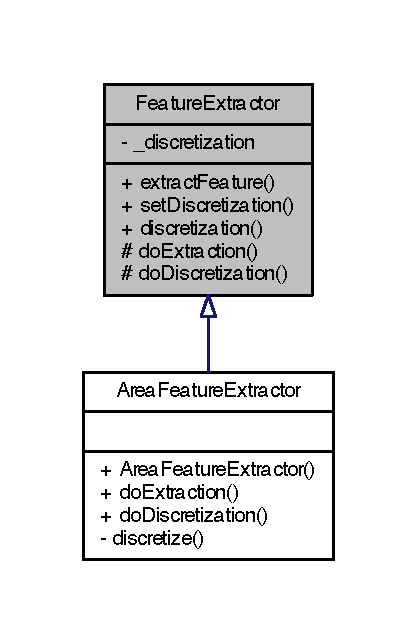
\includegraphics[width=200pt]{class_feature_extractor__inherit__graph}
\end{center}
\end{figure}


Collaboration diagram for Feature\+Extractor\+:
\nopagebreak
\begin{figure}[H]
\begin{center}
\leavevmode
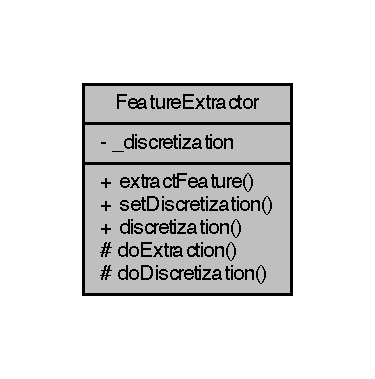
\includegraphics[width=180pt]{class_feature_extractor__coll__graph}
\end{center}
\end{figure}
\subsection*{Public Member Functions}
\begin{DoxyCompactItemize}
\item 
\hyperlink{class_feature}{Feature} \hyperlink{class_feature_extractor_a0bcc371c074b3aa6fa54b75b3657ffb0}{extract\+Feature} (\hyperlink{class_region}{Region} $\ast$r)
\item 
void \hyperlink{class_feature_extractor_a99ef3afd19f932dcb7dbb089e474d41b}{set\+Discretization} (int i)
\item 
int \hyperlink{class_feature_extractor_a1d800b4e5f3af7c758bfc5f157110681}{discretization} ()
\end{DoxyCompactItemize}
\subsection*{Protected Member Functions}
\begin{DoxyCompactItemize}
\item 
virtual Q\+Vector$<$ float $>$ \hyperlink{class_feature_extractor_aa5c094d54dc66b517ebde61fc9f1edf5}{do\+Extraction} (\hyperlink{class_region}{Region} $\ast$r)=0
\item 
virtual void \hyperlink{class_feature_extractor_ae0501342d6b872870af13cc5cd0a249f}{do\+Discretization} (Q\+Vector$<$ float $>$ \&feature, int \hyperlink{class_feature_extractor_a1d800b4e5f3af7c758bfc5f157110681}{discretization})=0
\end{DoxyCompactItemize}
\subsection*{Private Attributes}
\begin{DoxyCompactItemize}
\item 
int \hyperlink{class_feature_extractor_a76b9438b85a119c2ec4126b75c0486bf}{\+\_\+discretization}
\end{DoxyCompactItemize}


\subsection{Member Function Documentation}
\hypertarget{class_feature_extractor_a1d800b4e5f3af7c758bfc5f157110681}{\index{Feature\+Extractor@{Feature\+Extractor}!discretization@{discretization}}
\index{discretization@{discretization}!Feature\+Extractor@{Feature\+Extractor}}
\subsubsection[{discretization}]{\setlength{\rightskip}{0pt plus 5cm}int Feature\+Extractor\+::discretization (
\begin{DoxyParamCaption}
{}
\end{DoxyParamCaption}
)}}\label{class_feature_extractor_a1d800b4e5f3af7c758bfc5f157110681}


Here is the caller graph for this function\+:
\nopagebreak
\begin{figure}[H]
\begin{center}
\leavevmode
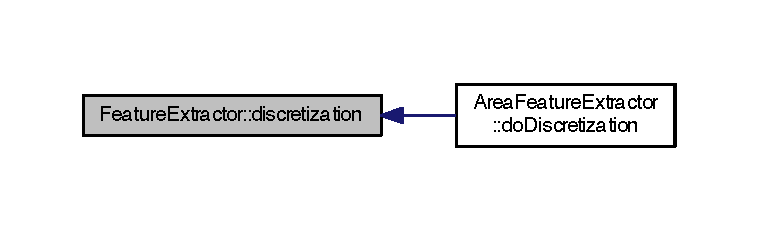
\includegraphics[width=350pt]{class_feature_extractor_a1d800b4e5f3af7c758bfc5f157110681_icgraph}
\end{center}
\end{figure}


\hypertarget{class_feature_extractor_ae0501342d6b872870af13cc5cd0a249f}{\index{Feature\+Extractor@{Feature\+Extractor}!do\+Discretization@{do\+Discretization}}
\index{do\+Discretization@{do\+Discretization}!Feature\+Extractor@{Feature\+Extractor}}
\subsubsection[{do\+Discretization}]{\setlength{\rightskip}{0pt plus 5cm}virtual void Feature\+Extractor\+::do\+Discretization (
\begin{DoxyParamCaption}
\item[{Q\+Vector$<$ float $>$ \&}]{feature, }
\item[{int}]{discretization}
\end{DoxyParamCaption}
)\hspace{0.3cm}{\ttfamily [protected]}, {\ttfamily [pure virtual]}}}\label{class_feature_extractor_ae0501342d6b872870af13cc5cd0a249f}


Implemented in \hyperlink{class_area_feature_extractor_a9969af2ec658c4404651cc13bef00089}{Area\+Feature\+Extractor}.



Here is the caller graph for this function\+:
\nopagebreak
\begin{figure}[H]
\begin{center}
\leavevmode
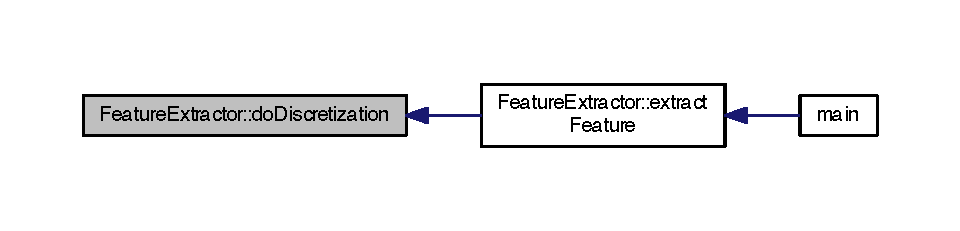
\includegraphics[width=350pt]{class_feature_extractor_ae0501342d6b872870af13cc5cd0a249f_icgraph}
\end{center}
\end{figure}


\hypertarget{class_feature_extractor_aa5c094d54dc66b517ebde61fc9f1edf5}{\index{Feature\+Extractor@{Feature\+Extractor}!do\+Extraction@{do\+Extraction}}
\index{do\+Extraction@{do\+Extraction}!Feature\+Extractor@{Feature\+Extractor}}
\subsubsection[{do\+Extraction}]{\setlength{\rightskip}{0pt plus 5cm}virtual Q\+Vector$<$float$>$ Feature\+Extractor\+::do\+Extraction (
\begin{DoxyParamCaption}
\item[{{\bf Region} $\ast$}]{r}
\end{DoxyParamCaption}
)\hspace{0.3cm}{\ttfamily [protected]}, {\ttfamily [pure virtual]}}}\label{class_feature_extractor_aa5c094d54dc66b517ebde61fc9f1edf5}


Implemented in \hyperlink{class_area_feature_extractor_a9dfd50444d94b1fd82fdd6ec0f9163c3}{Area\+Feature\+Extractor}.



Here is the caller graph for this function\+:
\nopagebreak
\begin{figure}[H]
\begin{center}
\leavevmode
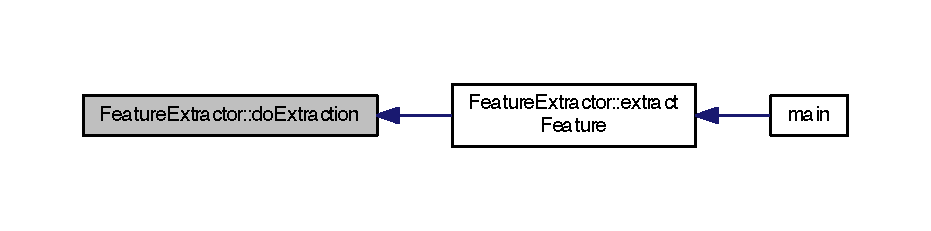
\includegraphics[width=350pt]{class_feature_extractor_aa5c094d54dc66b517ebde61fc9f1edf5_icgraph}
\end{center}
\end{figure}


\hypertarget{class_feature_extractor_a0bcc371c074b3aa6fa54b75b3657ffb0}{\index{Feature\+Extractor@{Feature\+Extractor}!extract\+Feature@{extract\+Feature}}
\index{extract\+Feature@{extract\+Feature}!Feature\+Extractor@{Feature\+Extractor}}
\subsubsection[{extract\+Feature}]{\setlength{\rightskip}{0pt plus 5cm}{\bf Feature} Feature\+Extractor\+::extract\+Feature (
\begin{DoxyParamCaption}
\item[{{\bf Region} $\ast$}]{r}
\end{DoxyParamCaption}
)}}\label{class_feature_extractor_a0bcc371c074b3aa6fa54b75b3657ffb0}


Here is the call graph for this function\+:
\nopagebreak
\begin{figure}[H]
\begin{center}
\leavevmode
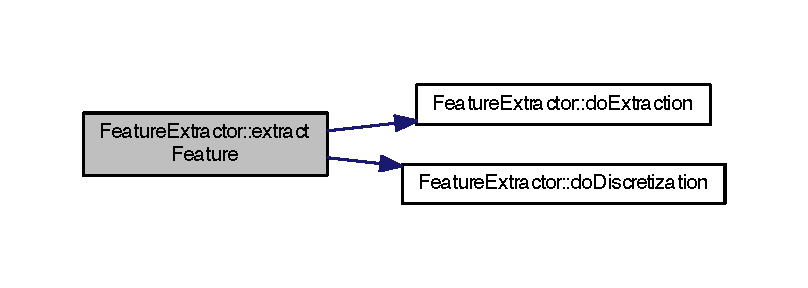
\includegraphics[width=350pt]{class_feature_extractor_a0bcc371c074b3aa6fa54b75b3657ffb0_cgraph}
\end{center}
\end{figure}




Here is the caller graph for this function\+:
\nopagebreak
\begin{figure}[H]
\begin{center}
\leavevmode
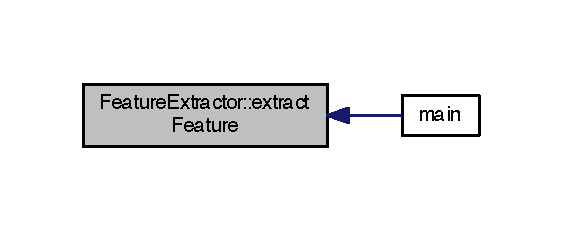
\includegraphics[width=270pt]{class_feature_extractor_a0bcc371c074b3aa6fa54b75b3657ffb0_icgraph}
\end{center}
\end{figure}


\hypertarget{class_feature_extractor_a99ef3afd19f932dcb7dbb089e474d41b}{\index{Feature\+Extractor@{Feature\+Extractor}!set\+Discretization@{set\+Discretization}}
\index{set\+Discretization@{set\+Discretization}!Feature\+Extractor@{Feature\+Extractor}}
\subsubsection[{set\+Discretization}]{\setlength{\rightskip}{0pt plus 5cm}void Feature\+Extractor\+::set\+Discretization (
\begin{DoxyParamCaption}
\item[{int}]{i}
\end{DoxyParamCaption}
)}}\label{class_feature_extractor_a99ef3afd19f932dcb7dbb089e474d41b}


Here is the caller graph for this function\+:
\nopagebreak
\begin{figure}[H]
\begin{center}
\leavevmode
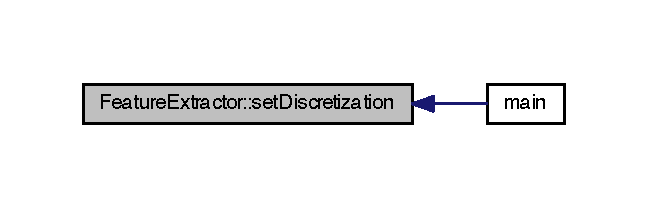
\includegraphics[width=311pt]{class_feature_extractor_a99ef3afd19f932dcb7dbb089e474d41b_icgraph}
\end{center}
\end{figure}




\subsection{Member Data Documentation}
\hypertarget{class_feature_extractor_a76b9438b85a119c2ec4126b75c0486bf}{\index{Feature\+Extractor@{Feature\+Extractor}!\+\_\+discretization@{\+\_\+discretization}}
\index{\+\_\+discretization@{\+\_\+discretization}!Feature\+Extractor@{Feature\+Extractor}}
\subsubsection[{\+\_\+discretization}]{\setlength{\rightskip}{0pt plus 5cm}int Feature\+Extractor\+::\+\_\+discretization\hspace{0.3cm}{\ttfamily [private]}}}\label{class_feature_extractor_a76b9438b85a119c2ec4126b75c0486bf}


The documentation for this class was generated from the following files\+:\begin{DoxyCompactItemize}
\item 
src/\hyperlink{_feature_extractor_8hpp}{Feature\+Extractor.\+hpp}\item 
src/\hyperlink{_feature_extractor_8cpp}{Feature\+Extractor.\+cpp}\end{DoxyCompactItemize}

\hypertarget{class_node}{\section{Node$<$ N\+O\+D\+E\+\_\+\+T\+Y\+P\+E, E\+D\+G\+E\+\_\+\+T\+Y\+P\+E $>$ Class Template Reference}
\label{class_node}\index{Node$<$ N\+O\+D\+E\+\_\+\+T\+Y\+P\+E, E\+D\+G\+E\+\_\+\+T\+Y\+P\+E $>$@{Node$<$ N\+O\+D\+E\+\_\+\+T\+Y\+P\+E, E\+D\+G\+E\+\_\+\+T\+Y\+P\+E $>$}}
}


{\ttfamily \#include $<$Node.\+hpp$>$}



Collaboration diagram for Node$<$ N\+O\+D\+E\+\_\+\+T\+Y\+P\+E, E\+D\+G\+E\+\_\+\+T\+Y\+P\+E $>$\+:
\nopagebreak
\begin{figure}[H]
\begin{center}
\leavevmode
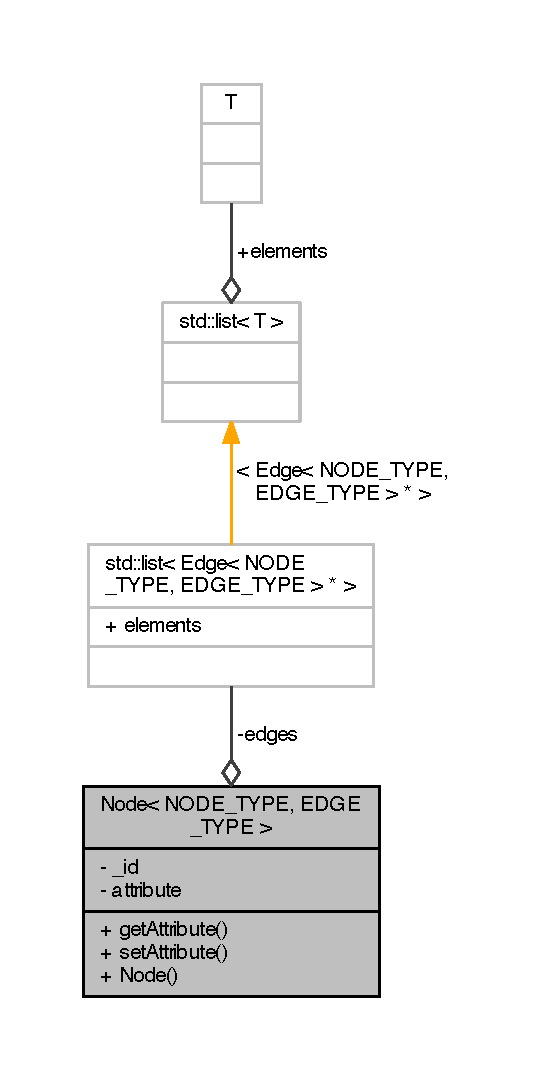
\includegraphics[width=222pt]{class_node__coll__graph}
\end{center}
\end{figure}
\subsection*{Public Member Functions}
\begin{DoxyCompactItemize}
\item 
N\+O\+D\+E\+\_\+\+T\+Y\+P\+E \hyperlink{class_node_a1272270025389e601164431b42ab5237}{get\+Attribute} ()
\item 
void \hyperlink{class_node_acb8f913ce2f995a6a14b9b05c60938f8}{set\+Attribute} (N\+O\+D\+E\+\_\+\+T\+Y\+P\+E attr)
\item 
\hyperlink{class_node_a94263af6c10cc9882d33918080dc722f}{Node} (N\+O\+D\+E\+\_\+\+T\+Y\+P\+E \hyperlink{class_node_a434cad0f70931bc3aaa048d52d0b0ee3}{attribute})
\end{DoxyCompactItemize}
\subsection*{Private Attributes}
\begin{DoxyCompactItemize}
\item 
int \hyperlink{class_node_a533ab17912d5b919a37ada31a8a78dc4}{\+\_\+id}
\item 
N\+O\+D\+E\+\_\+\+T\+Y\+P\+E \hyperlink{class_node_a434cad0f70931bc3aaa048d52d0b0ee3}{attribute}
\end{DoxyCompactItemize}


\subsection{Constructor \& Destructor Documentation}
\hypertarget{class_node_a94263af6c10cc9882d33918080dc722f}{\index{Node@{Node}!Node@{Node}}
\index{Node@{Node}!Node@{Node}}
\subsubsection[{Node}]{\setlength{\rightskip}{0pt plus 5cm}template$<$class N\+O\+D\+E\+\_\+\+T\+Y\+P\+E , class E\+D\+G\+E\+\_\+\+T\+Y\+P\+E $>$ {\bf Node}$<$ N\+O\+D\+E\+\_\+\+T\+Y\+P\+E, E\+D\+G\+E\+\_\+\+T\+Y\+P\+E $>$\+::{\bf Node} (
\begin{DoxyParamCaption}
\item[{N\+O\+D\+E\+\_\+\+T\+Y\+P\+E}]{attribute}
\end{DoxyParamCaption}
)}}\label{class_node_a94263af6c10cc9882d33918080dc722f}


\subsection{Member Function Documentation}
\hypertarget{class_node_a1272270025389e601164431b42ab5237}{\index{Node@{Node}!get\+Attribute@{get\+Attribute}}
\index{get\+Attribute@{get\+Attribute}!Node@{Node}}
\subsubsection[{get\+Attribute}]{\setlength{\rightskip}{0pt plus 5cm}template$<$class N\+O\+D\+E\+\_\+\+T\+Y\+P\+E , class E\+D\+G\+E\+\_\+\+T\+Y\+P\+E $>$ N\+O\+D\+E\+\_\+\+T\+Y\+P\+E {\bf Node}$<$ N\+O\+D\+E\+\_\+\+T\+Y\+P\+E, E\+D\+G\+E\+\_\+\+T\+Y\+P\+E $>$\+::get\+Attribute (
\begin{DoxyParamCaption}
{}
\end{DoxyParamCaption}
)}}\label{class_node_a1272270025389e601164431b42ab5237}


Here is the caller graph for this function\+:
\nopagebreak
\begin{figure}[H]
\begin{center}
\leavevmode
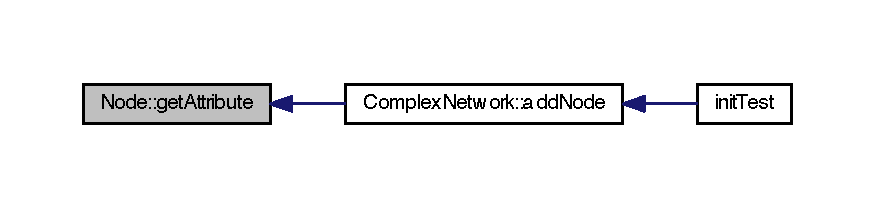
\includegraphics[width=350pt]{class_node_a1272270025389e601164431b42ab5237_icgraph}
\end{center}
\end{figure}


\hypertarget{class_node_acb8f913ce2f995a6a14b9b05c60938f8}{\index{Node@{Node}!set\+Attribute@{set\+Attribute}}
\index{set\+Attribute@{set\+Attribute}!Node@{Node}}
\subsubsection[{set\+Attribute}]{\setlength{\rightskip}{0pt plus 5cm}template$<$class N\+O\+D\+E\+\_\+\+T\+Y\+P\+E , class E\+D\+G\+E\+\_\+\+T\+Y\+P\+E $>$ void {\bf Node}$<$ N\+O\+D\+E\+\_\+\+T\+Y\+P\+E, E\+D\+G\+E\+\_\+\+T\+Y\+P\+E $>$\+::set\+Attribute (
\begin{DoxyParamCaption}
\item[{N\+O\+D\+E\+\_\+\+T\+Y\+P\+E}]{attr}
\end{DoxyParamCaption}
)}}\label{class_node_acb8f913ce2f995a6a14b9b05c60938f8}


\subsection{Member Data Documentation}
\hypertarget{class_node_a533ab17912d5b919a37ada31a8a78dc4}{\index{Node@{Node}!\+\_\+id@{\+\_\+id}}
\index{\+\_\+id@{\+\_\+id}!Node@{Node}}
\subsubsection[{\+\_\+id}]{\setlength{\rightskip}{0pt plus 5cm}template$<$class N\+O\+D\+E\+\_\+\+T\+Y\+P\+E, class E\+D\+G\+E\+\_\+\+T\+Y\+P\+E$>$ int {\bf Node}$<$ N\+O\+D\+E\+\_\+\+T\+Y\+P\+E, E\+D\+G\+E\+\_\+\+T\+Y\+P\+E $>$\+::\+\_\+id\hspace{0.3cm}{\ttfamily [private]}}}\label{class_node_a533ab17912d5b919a37ada31a8a78dc4}
\hypertarget{class_node_a434cad0f70931bc3aaa048d52d0b0ee3}{\index{Node@{Node}!attribute@{attribute}}
\index{attribute@{attribute}!Node@{Node}}
\subsubsection[{attribute}]{\setlength{\rightskip}{0pt plus 5cm}template$<$class N\+O\+D\+E\+\_\+\+T\+Y\+P\+E, class E\+D\+G\+E\+\_\+\+T\+Y\+P\+E$>$ N\+O\+D\+E\+\_\+\+T\+Y\+P\+E {\bf Node}$<$ N\+O\+D\+E\+\_\+\+T\+Y\+P\+E, E\+D\+G\+E\+\_\+\+T\+Y\+P\+E $>$\+::attribute\hspace{0.3cm}{\ttfamily [private]}}}\label{class_node_a434cad0f70931bc3aaa048d52d0b0ee3}


The documentation for this class was generated from the following file\+:\begin{DoxyCompactItemize}
\item 
src/\hyperlink{_node_8hpp}{Node.\+hpp}\end{DoxyCompactItemize}

\hypertarget{classnode__t}{\section{node\+\_\+t Class Reference}
\label{classnode__t}\index{node\+\_\+t@{node\+\_\+t}}
}
\subsection*{Public Member Functions}
\begin{DoxyCompactItemize}
\item 
bool \hyperlink{classnode__t_ab77397ae86ade5bb789b138676567ce6}{operator$<$} (const \hyperlink{classnode__t}{node\+\_\+t} \&other) const 
\item 
\hyperlink{classnode__t_a0cd5044c3a9307c565c9a86136fbf1dd}{node\+\_\+t} (int \hyperlink{classnode__t_a28f58cd3011e9e060f41ef08a5e5c12b}{v1}=0, int \hyperlink{classnode__t_ac331c5d766e147caf0b97154ef8395db}{v2}=0)
\end{DoxyCompactItemize}
\subsection*{Public Attributes}
\begin{DoxyCompactItemize}
\item 
int \hyperlink{classnode__t_a28f58cd3011e9e060f41ef08a5e5c12b}{v1}
\item 
int \hyperlink{classnode__t_ac331c5d766e147caf0b97154ef8395db}{v2}
\end{DoxyCompactItemize}


Collaboration diagram for node\+\_\+t\+:\nopagebreak
\begin{figure}[H]
\begin{center}
\leavevmode
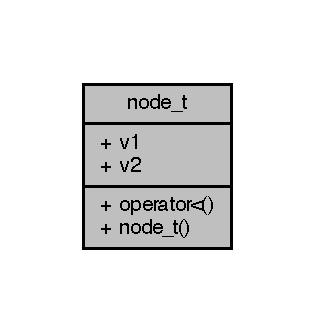
\includegraphics[width=151pt]{classnode__t__coll__graph}
\end{center}
\end{figure}


\subsection{Constructor \& Destructor Documentation}
\hypertarget{classnode__t_a0cd5044c3a9307c565c9a86136fbf1dd}{\index{node\+\_\+t@{node\+\_\+t}!node\+\_\+t@{node\+\_\+t}}
\index{node\+\_\+t@{node\+\_\+t}!node\+\_\+t@{node\+\_\+t}}
\subsubsection[{node\+\_\+t}]{\setlength{\rightskip}{0pt plus 5cm}node\+\_\+t\+::node\+\_\+t (
\begin{DoxyParamCaption}
\item[{int}]{v1 = {\ttfamily 0}, }
\item[{int}]{v2 = {\ttfamily 0}}
\end{DoxyParamCaption}
)\hspace{0.3cm}{\ttfamily [inline]}}}\label{classnode__t_a0cd5044c3a9307c565c9a86136fbf1dd}


\subsection{Member Function Documentation}
\hypertarget{classnode__t_ab77397ae86ade5bb789b138676567ce6}{\index{node\+\_\+t@{node\+\_\+t}!operator$<$@{operator$<$}}
\index{operator$<$@{operator$<$}!node\+\_\+t@{node\+\_\+t}}
\subsubsection[{operator$<$}]{\setlength{\rightskip}{0pt plus 5cm}bool node\+\_\+t\+::operator$<$ (
\begin{DoxyParamCaption}
\item[{const {\bf node\+\_\+t} \&}]{other}
\end{DoxyParamCaption}
) const\hspace{0.3cm}{\ttfamily [inline]}}}\label{classnode__t_ab77397ae86ade5bb789b138676567ce6}


\subsection{Member Data Documentation}
\hypertarget{classnode__t_a28f58cd3011e9e060f41ef08a5e5c12b}{\index{node\+\_\+t@{node\+\_\+t}!v1@{v1}}
\index{v1@{v1}!node\+\_\+t@{node\+\_\+t}}
\subsubsection[{v1}]{\setlength{\rightskip}{0pt plus 5cm}int node\+\_\+t\+::v1}}\label{classnode__t_a28f58cd3011e9e060f41ef08a5e5c12b}
\hypertarget{classnode__t_ac331c5d766e147caf0b97154ef8395db}{\index{node\+\_\+t@{node\+\_\+t}!v2@{v2}}
\index{v2@{v2}!node\+\_\+t@{node\+\_\+t}}
\subsubsection[{v2}]{\setlength{\rightskip}{0pt plus 5cm}int node\+\_\+t\+::v2}}\label{classnode__t_ac331c5d766e147caf0b97154ef8395db}


The documentation for this class was generated from the following file\+:\begin{DoxyCompactItemize}
\item 
Sources/\+Tests/\+Complex\+Network\+Resources\+Test/\hyperlink{_complex_network_resources_test_8cpp}{Complex\+Network\+Resources\+Test.\+cpp}\end{DoxyCompactItemize}

\hypertarget{class_region}{\section{Region Class Reference}
\label{class_region}\index{Region@{Region}}
}


{\ttfamily \#include $<$Region.\+hpp$>$}



Collaboration diagram for Region\+:
\nopagebreak
\begin{figure}[H]
\begin{center}
\leavevmode
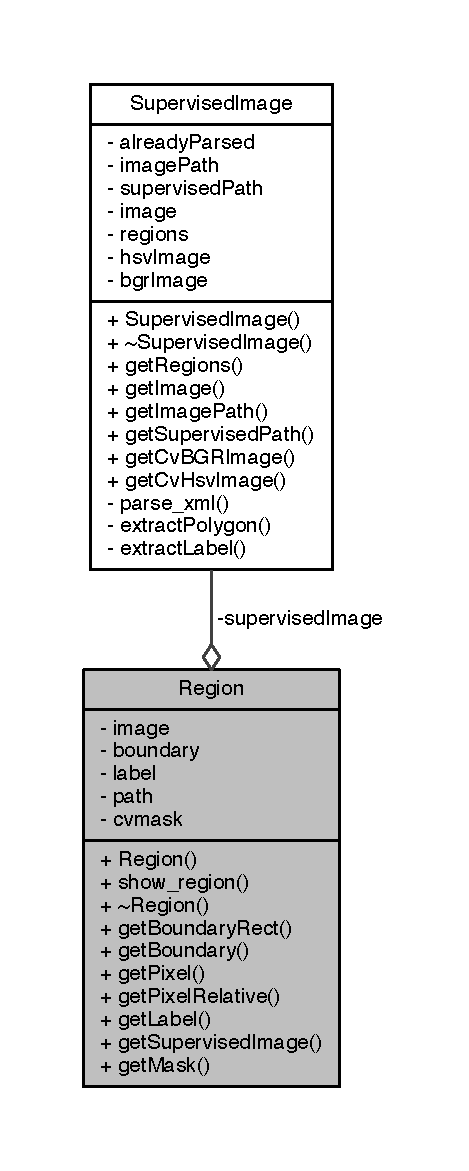
\includegraphics[width=185pt]{class_region__coll__graph}
\end{center}
\end{figure}
\subsection*{Public Member Functions}
\begin{DoxyCompactItemize}
\item 
\hyperlink{class_region_a0e9c8974b3be20ce12a4b823f9f3f636}{Region} (Q\+Image $\ast$\hyperlink{class_region_a090b8bc9a8c73f8f874d8d439a0843be}{image}, Q\+Polygon \hyperlink{class_region_a4a59ef37013f3a6515a79317b0f0b4c0}{boundary}, Q\+String \hyperlink{class_region_afcc063386e02be883d71eaf5bcef2a55}{label})
\item 
void \hyperlink{class_region_ad2572028c1a4653a14dbfb1b622aa03e}{show\+\_\+region} ()
\item 
\hyperlink{class_region_a3c3670fff78f7511d156e3b2f0bc6266}{$\sim$\+Region} ()
\item 
Q\+Rect \hyperlink{class_region_a12c653b5aa89c899e2680c9dc1bbf46d}{get\+Boundary\+Rect} () const 
\item 
Q\+Rgb \hyperlink{class_region_acc0edaac14854ccc448f419844a722bf}{get\+Pixel} (int x, int y, bool $\ast$inside\+Region=N\+U\+L\+L) const 
\item 
Q\+Rgb \hyperlink{class_region_a421786f57555f6348ece3fa33eb86594}{get\+Pixel\+Relative} (int x, int y, bool $\ast$inside\+Region=N\+U\+L\+L) const 
\item 
Q\+String \hyperlink{class_region_a69d5acb5d1d81b50f225817217f60fdd}{get\+Label} () const 
\end{DoxyCompactItemize}
\subsection*{Private Attributes}
\begin{DoxyCompactItemize}
\item 
Q\+Image $\ast$ \hyperlink{class_region_a090b8bc9a8c73f8f874d8d439a0843be}{image}
\item 
Q\+Polygon \hyperlink{class_region_a4a59ef37013f3a6515a79317b0f0b4c0}{boundary}
\item 
Q\+String \hyperlink{class_region_afcc063386e02be883d71eaf5bcef2a55}{label}
\item 
Q\+Label $\ast$ \hyperlink{class_region_a31cb137d1eab434b70aaa95633e704fe}{l} =N\+U\+L\+L
\end{DoxyCompactItemize}


\subsection{Constructor \& Destructor Documentation}
\hypertarget{class_region_a0e9c8974b3be20ce12a4b823f9f3f636}{\index{Region@{Region}!Region@{Region}}
\index{Region@{Region}!Region@{Region}}
\subsubsection[{Region}]{\setlength{\rightskip}{0pt plus 5cm}Region\+::\+Region (
\begin{DoxyParamCaption}
\item[{Q\+Image $\ast$}]{image, }
\item[{Q\+Polygon}]{boundary, }
\item[{Q\+String}]{label}
\end{DoxyParamCaption}
)}}\label{class_region_a0e9c8974b3be20ce12a4b823f9f3f636}
\hypertarget{class_region_a3c3670fff78f7511d156e3b2f0bc6266}{\index{Region@{Region}!````~Region@{$\sim$\+Region}}
\index{````~Region@{$\sim$\+Region}!Region@{Region}}
\subsubsection[{$\sim$\+Region}]{\setlength{\rightskip}{0pt plus 5cm}Region\+::$\sim$\+Region (
\begin{DoxyParamCaption}
{}
\end{DoxyParamCaption}
)}}\label{class_region_a3c3670fff78f7511d156e3b2f0bc6266}


\subsection{Member Function Documentation}
\hypertarget{class_region_a12c653b5aa89c899e2680c9dc1bbf46d}{\index{Region@{Region}!get\+Boundary\+Rect@{get\+Boundary\+Rect}}
\index{get\+Boundary\+Rect@{get\+Boundary\+Rect}!Region@{Region}}
\subsubsection[{get\+Boundary\+Rect}]{\setlength{\rightskip}{0pt plus 5cm}Q\+Rect Region\+::get\+Boundary\+Rect (
\begin{DoxyParamCaption}
{}
\end{DoxyParamCaption}
) const}}\label{class_region_a12c653b5aa89c899e2680c9dc1bbf46d}


Here is the caller graph for this function\+:
\nopagebreak
\begin{figure}[H]
\begin{center}
\leavevmode
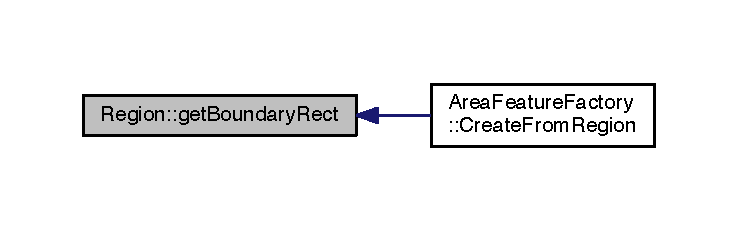
\includegraphics[width=350pt]{class_region_a12c653b5aa89c899e2680c9dc1bbf46d_icgraph}
\end{center}
\end{figure}


\hypertarget{class_region_a69d5acb5d1d81b50f225817217f60fdd}{\index{Region@{Region}!get\+Label@{get\+Label}}
\index{get\+Label@{get\+Label}!Region@{Region}}
\subsubsection[{get\+Label}]{\setlength{\rightskip}{0pt plus 5cm}Q\+String Region\+::get\+Label (
\begin{DoxyParamCaption}
{}
\end{DoxyParamCaption}
) const}}\label{class_region_a69d5acb5d1d81b50f225817217f60fdd}
\hypertarget{class_region_acc0edaac14854ccc448f419844a722bf}{\index{Region@{Region}!get\+Pixel@{get\+Pixel}}
\index{get\+Pixel@{get\+Pixel}!Region@{Region}}
\subsubsection[{get\+Pixel}]{\setlength{\rightskip}{0pt plus 5cm}Q\+Rgb Region\+::get\+Pixel (
\begin{DoxyParamCaption}
\item[{int}]{x, }
\item[{int}]{y, }
\item[{bool $\ast$}]{inside\+Region = {\ttfamily NULL}}
\end{DoxyParamCaption}
) const}}\label{class_region_acc0edaac14854ccc448f419844a722bf}


Here is the caller graph for this function\+:
\nopagebreak
\begin{figure}[H]
\begin{center}
\leavevmode
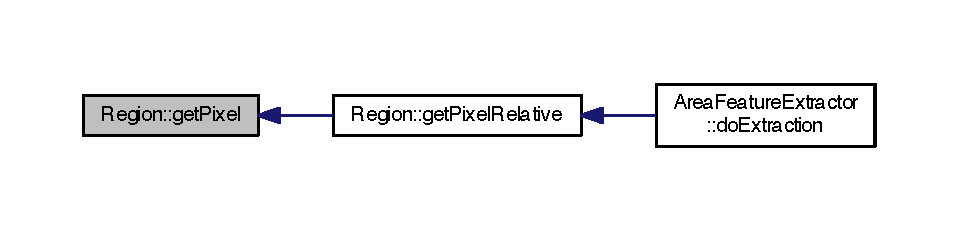
\includegraphics[width=350pt]{class_region_acc0edaac14854ccc448f419844a722bf_icgraph}
\end{center}
\end{figure}


\hypertarget{class_region_a421786f57555f6348ece3fa33eb86594}{\index{Region@{Region}!get\+Pixel\+Relative@{get\+Pixel\+Relative}}
\index{get\+Pixel\+Relative@{get\+Pixel\+Relative}!Region@{Region}}
\subsubsection[{get\+Pixel\+Relative}]{\setlength{\rightskip}{0pt plus 5cm}Q\+Rgb Region\+::get\+Pixel\+Relative (
\begin{DoxyParamCaption}
\item[{int}]{x, }
\item[{int}]{y, }
\item[{bool $\ast$}]{inside\+Region = {\ttfamily NULL}}
\end{DoxyParamCaption}
) const}}\label{class_region_a421786f57555f6348ece3fa33eb86594}


Here is the call graph for this function\+:
\nopagebreak
\begin{figure}[H]
\begin{center}
\leavevmode
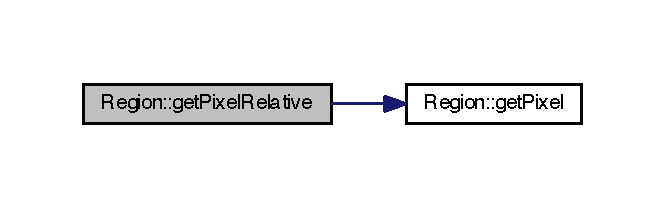
\includegraphics[width=319pt]{class_region_a421786f57555f6348ece3fa33eb86594_cgraph}
\end{center}
\end{figure}




Here is the caller graph for this function\+:
\nopagebreak
\begin{figure}[H]
\begin{center}
\leavevmode
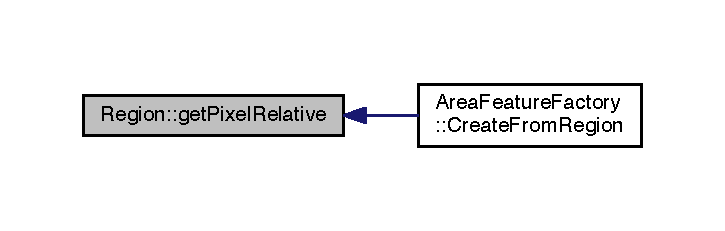
\includegraphics[width=350pt]{class_region_a421786f57555f6348ece3fa33eb86594_icgraph}
\end{center}
\end{figure}


\hypertarget{class_region_ad2572028c1a4653a14dbfb1b622aa03e}{\index{Region@{Region}!show\+\_\+region@{show\+\_\+region}}
\index{show\+\_\+region@{show\+\_\+region}!Region@{Region}}
\subsubsection[{show\+\_\+region}]{\setlength{\rightskip}{0pt plus 5cm}void Region\+::show\+\_\+region (
\begin{DoxyParamCaption}
{}
\end{DoxyParamCaption}
)}}\label{class_region_ad2572028c1a4653a14dbfb1b622aa03e}


\subsection{Member Data Documentation}
\hypertarget{class_region_a4a59ef37013f3a6515a79317b0f0b4c0}{\index{Region@{Region}!boundary@{boundary}}
\index{boundary@{boundary}!Region@{Region}}
\subsubsection[{boundary}]{\setlength{\rightskip}{0pt plus 5cm}Q\+Polygon Region\+::boundary\hspace{0.3cm}{\ttfamily [private]}}}\label{class_region_a4a59ef37013f3a6515a79317b0f0b4c0}
\hypertarget{class_region_a090b8bc9a8c73f8f874d8d439a0843be}{\index{Region@{Region}!image@{image}}
\index{image@{image}!Region@{Region}}
\subsubsection[{image}]{\setlength{\rightskip}{0pt plus 5cm}Q\+Image$\ast$ Region\+::image\hspace{0.3cm}{\ttfamily [private]}}}\label{class_region_a090b8bc9a8c73f8f874d8d439a0843be}
\hypertarget{class_region_a31cb137d1eab434b70aaa95633e704fe}{\index{Region@{Region}!l@{l}}
\index{l@{l}!Region@{Region}}
\subsubsection[{l}]{\setlength{\rightskip}{0pt plus 5cm}Q\+Label$\ast$ Region\+::l =N\+U\+L\+L\hspace{0.3cm}{\ttfamily [private]}}}\label{class_region_a31cb137d1eab434b70aaa95633e704fe}
\hypertarget{class_region_afcc063386e02be883d71eaf5bcef2a55}{\index{Region@{Region}!label@{label}}
\index{label@{label}!Region@{Region}}
\subsubsection[{label}]{\setlength{\rightskip}{0pt plus 5cm}Q\+String Region\+::label\hspace{0.3cm}{\ttfamily [private]}}}\label{class_region_afcc063386e02be883d71eaf5bcef2a55}


The documentation for this class was generated from the following files\+:\begin{DoxyCompactItemize}
\item 
src/\hyperlink{_region_8hpp}{Region.\+hpp}\item 
src/\hyperlink{_region_8cpp}{Region.\+cpp}\end{DoxyCompactItemize}

\hypertarget{class_sun_database_reader}{\section{Sun\+Database\+Reader Class Reference}
\label{class_sun_database_reader}\index{Sun\+Database\+Reader@{Sun\+Database\+Reader}}
}


{\ttfamily \#include $<$Sun\+Database\+Reader.\+hpp$>$}

\subsection*{Public Member Functions}
\begin{DoxyCompactItemize}
\item 
\hyperlink{class_sun_database_reader_a7165e085898b5e329402b8acc17f3e0e}{Sun\+Database\+Reader} (Q\+String \hyperlink{class_sun_database_reader_a6bfc31b2ba24be2b3e18c32e0d343d70}{source\+Dir})
\item 
bool \hyperlink{class_sun_database_reader_a5530b88632379c373b592d5128c2999f}{has\+Next} () const 
\item 
\hyperlink{class_supervised_image}{Supervised\+Image} \hyperlink{class_sun_database_reader_a92a92483d9b4eadc4008f29a89068e71}{read\+Next} ()
\item 
bool \hyperlink{class_sun_database_reader_abe3da501f9df416baf1b077e4d4eadb8}{has\+Previous} () const 
\item 
\hyperlink{class_supervised_image}{Supervised\+Image} \hyperlink{class_sun_database_reader_a8109235f5d4a3e7763afe22f4c8c37a0}{read\+Previous} ()
\item 
unsigned int \hyperlink{class_sun_database_reader_a8d704a7121e1babebe4673049d37a095}{get\+Total} () const 
\end{DoxyCompactItemize}
\subsection*{Private Member Functions}
\begin{DoxyCompactItemize}
\item 
void \hyperlink{class_sun_database_reader_aefbdf63eaff6755bb3dee0ef8687b3aa}{discover\+\_\+files} (Q\+String)
\end{DoxyCompactItemize}
\subsection*{Private Attributes}
\begin{DoxyCompactItemize}
\item 
Q\+Dir \hyperlink{class_sun_database_reader_a6bfc31b2ba24be2b3e18c32e0d343d70}{source\+Dir}
\item 
Q\+List$<$ Q\+String $>$ \hyperlink{class_sun_database_reader_a155716f43a3dc33e1a4d0a2a4a9f3ff1}{image\+\_\+files}
\item 
Q\+List$<$ Q\+String $>$ \hyperlink{class_sun_database_reader_ac5afd4950a668e5cff2bc5c6ea024b60}{supervision\+\_\+files}
\item 
Q\+List$<$ Q\+String $>$\+::iterator \hyperlink{class_sun_database_reader_a227d88c9c5c3d37b0f27123027c0b00e}{image\+\_\+files\+\_\+it}
\item 
Q\+List$<$ Q\+String $>$\+::iterator \hyperlink{class_sun_database_reader_a78e30a0ac9cfa46c23dbdf8d37226b51}{supervision\+\_\+files\+\_\+it}
\item 
bool \hyperlink{class_sun_database_reader_aa0b0c1f783f4382a9c8b10a1de1fec71}{started}
\end{DoxyCompactItemize}


Inheritance diagram for Sun\+Database\+Reader\+:\nopagebreak
\begin{figure}[H]
\begin{center}
\leavevmode
\includegraphics[width=205pt]{class_sun_database_reader__inherit__graph}
\end{center}
\end{figure}


Collaboration diagram for Sun\+Database\+Reader\+:\nopagebreak
\begin{figure}[H]
\begin{center}
\leavevmode
\includegraphics[width=205pt]{class_sun_database_reader__coll__graph}
\end{center}
\end{figure}


\subsection{Constructor \& Destructor Documentation}
\hypertarget{class_sun_database_reader_a7165e085898b5e329402b8acc17f3e0e}{\index{Sun\+Database\+Reader@{Sun\+Database\+Reader}!Sun\+Database\+Reader@{Sun\+Database\+Reader}}
\index{Sun\+Database\+Reader@{Sun\+Database\+Reader}!Sun\+Database\+Reader@{Sun\+Database\+Reader}}
\subsubsection[{Sun\+Database\+Reader}]{\setlength{\rightskip}{0pt plus 5cm}Sun\+Database\+Reader\+::\+Sun\+Database\+Reader (
\begin{DoxyParamCaption}
\item[{Q\+String}]{source\+Dir}
\end{DoxyParamCaption}
)}}\label{class_sun_database_reader_a7165e085898b5e329402b8acc17f3e0e}


Here is the call graph for this function\+:\nopagebreak
\begin{figure}[H]
\begin{center}
\leavevmode
\includegraphics[width=344pt]{class_sun_database_reader_a7165e085898b5e329402b8acc17f3e0e_cgraph}
\end{center}
\end{figure}




\subsection{Member Function Documentation}
\hypertarget{class_sun_database_reader_aefbdf63eaff6755bb3dee0ef8687b3aa}{\index{Sun\+Database\+Reader@{Sun\+Database\+Reader}!discover\+\_\+files@{discover\+\_\+files}}
\index{discover\+\_\+files@{discover\+\_\+files}!Sun\+Database\+Reader@{Sun\+Database\+Reader}}
\subsubsection[{discover\+\_\+files}]{\setlength{\rightskip}{0pt plus 5cm}void Sun\+Database\+Reader\+::discover\+\_\+files (
\begin{DoxyParamCaption}
\item[{Q\+String}]{path}
\end{DoxyParamCaption}
)\hspace{0.3cm}{\ttfamily [private]}}}\label{class_sun_database_reader_aefbdf63eaff6755bb3dee0ef8687b3aa}


Here is the caller graph for this function\+:\nopagebreak
\begin{figure}[H]
\begin{center}
\leavevmode
\includegraphics[width=344pt]{class_sun_database_reader_aefbdf63eaff6755bb3dee0ef8687b3aa_icgraph}
\end{center}
\end{figure}


\hypertarget{class_sun_database_reader_a8d704a7121e1babebe4673049d37a095}{\index{Sun\+Database\+Reader@{Sun\+Database\+Reader}!get\+Total@{get\+Total}}
\index{get\+Total@{get\+Total}!Sun\+Database\+Reader@{Sun\+Database\+Reader}}
\subsubsection[{get\+Total}]{\setlength{\rightskip}{0pt plus 5cm}unsigned int Sun\+Database\+Reader\+::get\+Total (
\begin{DoxyParamCaption}
{}
\end{DoxyParamCaption}
) const\hspace{0.3cm}{\ttfamily [virtual]}}}\label{class_sun_database_reader_a8d704a7121e1babebe4673049d37a095}


Implements \hyperlink{class_database_reader_abd37fa505553101bd8e18fd52547b7ee}{Database\+Reader}.



Here is the caller graph for this function\+:\nopagebreak
\begin{figure}[H]
\begin{center}
\leavevmode
\includegraphics[width=350pt]{class_sun_database_reader_a8d704a7121e1babebe4673049d37a095_icgraph}
\end{center}
\end{figure}


\hypertarget{class_sun_database_reader_a5530b88632379c373b592d5128c2999f}{\index{Sun\+Database\+Reader@{Sun\+Database\+Reader}!has\+Next@{has\+Next}}
\index{has\+Next@{has\+Next}!Sun\+Database\+Reader@{Sun\+Database\+Reader}}
\subsubsection[{has\+Next}]{\setlength{\rightskip}{0pt plus 5cm}bool Sun\+Database\+Reader\+::has\+Next (
\begin{DoxyParamCaption}
{}
\end{DoxyParamCaption}
) const\hspace{0.3cm}{\ttfamily [virtual]}}}\label{class_sun_database_reader_a5530b88632379c373b592d5128c2999f}


Implements \hyperlink{class_database_reader_a406c8a783b41f31a273ed9c761bf33fe}{Database\+Reader}.



Here is the caller graph for this function\+:\nopagebreak
\begin{figure}[H]
\begin{center}
\leavevmode
\includegraphics[width=350pt]{class_sun_database_reader_a5530b88632379c373b592d5128c2999f_icgraph}
\end{center}
\end{figure}


\hypertarget{class_sun_database_reader_abe3da501f9df416baf1b077e4d4eadb8}{\index{Sun\+Database\+Reader@{Sun\+Database\+Reader}!has\+Previous@{has\+Previous}}
\index{has\+Previous@{has\+Previous}!Sun\+Database\+Reader@{Sun\+Database\+Reader}}
\subsubsection[{has\+Previous}]{\setlength{\rightskip}{0pt plus 5cm}bool Sun\+Database\+Reader\+::has\+Previous (
\begin{DoxyParamCaption}
{}
\end{DoxyParamCaption}
) const\hspace{0.3cm}{\ttfamily [virtual]}}}\label{class_sun_database_reader_abe3da501f9df416baf1b077e4d4eadb8}


Implements \hyperlink{class_database_reader_acc71ed6c7af71bdc66b4b6eee3598506}{Database\+Reader}.

\hypertarget{class_sun_database_reader_a92a92483d9b4eadc4008f29a89068e71}{\index{Sun\+Database\+Reader@{Sun\+Database\+Reader}!read\+Next@{read\+Next}}
\index{read\+Next@{read\+Next}!Sun\+Database\+Reader@{Sun\+Database\+Reader}}
\subsubsection[{read\+Next}]{\setlength{\rightskip}{0pt plus 5cm}{\bf Supervised\+Image} Sun\+Database\+Reader\+::read\+Next (
\begin{DoxyParamCaption}
{}
\end{DoxyParamCaption}
)\hspace{0.3cm}{\ttfamily [virtual]}}}\label{class_sun_database_reader_a92a92483d9b4eadc4008f29a89068e71}


Implements \hyperlink{class_database_reader_a4bf8a5faaaeaa057050e9c7ca4370081}{Database\+Reader}.



Here is the caller graph for this function\+:\nopagebreak
\begin{figure}[H]
\begin{center}
\leavevmode
\includegraphics[width=350pt]{class_sun_database_reader_a92a92483d9b4eadc4008f29a89068e71_icgraph}
\end{center}
\end{figure}


\hypertarget{class_sun_database_reader_a8109235f5d4a3e7763afe22f4c8c37a0}{\index{Sun\+Database\+Reader@{Sun\+Database\+Reader}!read\+Previous@{read\+Previous}}
\index{read\+Previous@{read\+Previous}!Sun\+Database\+Reader@{Sun\+Database\+Reader}}
\subsubsection[{read\+Previous}]{\setlength{\rightskip}{0pt plus 5cm}{\bf Supervised\+Image} Sun\+Database\+Reader\+::read\+Previous (
\begin{DoxyParamCaption}
{}
\end{DoxyParamCaption}
)\hspace{0.3cm}{\ttfamily [virtual]}}}\label{class_sun_database_reader_a8109235f5d4a3e7763afe22f4c8c37a0}


Implements \hyperlink{class_database_reader_a762e5d499c9d60e5ba85344c1c7c2c8c}{Database\+Reader}.



Here is the caller graph for this function\+:\nopagebreak
\begin{figure}[H]
\begin{center}
\leavevmode
\includegraphics[width=350pt]{class_sun_database_reader_a8109235f5d4a3e7763afe22f4c8c37a0_icgraph}
\end{center}
\end{figure}




\subsection{Member Data Documentation}
\hypertarget{class_sun_database_reader_a155716f43a3dc33e1a4d0a2a4a9f3ff1}{\index{Sun\+Database\+Reader@{Sun\+Database\+Reader}!image\+\_\+files@{image\+\_\+files}}
\index{image\+\_\+files@{image\+\_\+files}!Sun\+Database\+Reader@{Sun\+Database\+Reader}}
\subsubsection[{image\+\_\+files}]{\setlength{\rightskip}{0pt plus 5cm}Q\+List$<$Q\+String$>$ Sun\+Database\+Reader\+::image\+\_\+files\hspace{0.3cm}{\ttfamily [private]}}}\label{class_sun_database_reader_a155716f43a3dc33e1a4d0a2a4a9f3ff1}
\hypertarget{class_sun_database_reader_a227d88c9c5c3d37b0f27123027c0b00e}{\index{Sun\+Database\+Reader@{Sun\+Database\+Reader}!image\+\_\+files\+\_\+it@{image\+\_\+files\+\_\+it}}
\index{image\+\_\+files\+\_\+it@{image\+\_\+files\+\_\+it}!Sun\+Database\+Reader@{Sun\+Database\+Reader}}
\subsubsection[{image\+\_\+files\+\_\+it}]{\setlength{\rightskip}{0pt plus 5cm}Q\+List$<$Q\+String$>$\+::iterator Sun\+Database\+Reader\+::image\+\_\+files\+\_\+it\hspace{0.3cm}{\ttfamily [private]}}}\label{class_sun_database_reader_a227d88c9c5c3d37b0f27123027c0b00e}
\hypertarget{class_sun_database_reader_a6bfc31b2ba24be2b3e18c32e0d343d70}{\index{Sun\+Database\+Reader@{Sun\+Database\+Reader}!source\+Dir@{source\+Dir}}
\index{source\+Dir@{source\+Dir}!Sun\+Database\+Reader@{Sun\+Database\+Reader}}
\subsubsection[{source\+Dir}]{\setlength{\rightskip}{0pt plus 5cm}Q\+Dir Sun\+Database\+Reader\+::source\+Dir\hspace{0.3cm}{\ttfamily [private]}}}\label{class_sun_database_reader_a6bfc31b2ba24be2b3e18c32e0d343d70}
\hypertarget{class_sun_database_reader_aa0b0c1f783f4382a9c8b10a1de1fec71}{\index{Sun\+Database\+Reader@{Sun\+Database\+Reader}!started@{started}}
\index{started@{started}!Sun\+Database\+Reader@{Sun\+Database\+Reader}}
\subsubsection[{started}]{\setlength{\rightskip}{0pt plus 5cm}bool Sun\+Database\+Reader\+::started\hspace{0.3cm}{\ttfamily [private]}}}\label{class_sun_database_reader_aa0b0c1f783f4382a9c8b10a1de1fec71}
\hypertarget{class_sun_database_reader_ac5afd4950a668e5cff2bc5c6ea024b60}{\index{Sun\+Database\+Reader@{Sun\+Database\+Reader}!supervision\+\_\+files@{supervision\+\_\+files}}
\index{supervision\+\_\+files@{supervision\+\_\+files}!Sun\+Database\+Reader@{Sun\+Database\+Reader}}
\subsubsection[{supervision\+\_\+files}]{\setlength{\rightskip}{0pt plus 5cm}Q\+List$<$Q\+String$>$ Sun\+Database\+Reader\+::supervision\+\_\+files\hspace{0.3cm}{\ttfamily [private]}}}\label{class_sun_database_reader_ac5afd4950a668e5cff2bc5c6ea024b60}
\hypertarget{class_sun_database_reader_a78e30a0ac9cfa46c23dbdf8d37226b51}{\index{Sun\+Database\+Reader@{Sun\+Database\+Reader}!supervision\+\_\+files\+\_\+it@{supervision\+\_\+files\+\_\+it}}
\index{supervision\+\_\+files\+\_\+it@{supervision\+\_\+files\+\_\+it}!Sun\+Database\+Reader@{Sun\+Database\+Reader}}
\subsubsection[{supervision\+\_\+files\+\_\+it}]{\setlength{\rightskip}{0pt plus 5cm}Q\+List$<$Q\+String$>$\+::iterator Sun\+Database\+Reader\+::supervision\+\_\+files\+\_\+it\hspace{0.3cm}{\ttfamily [private]}}}\label{class_sun_database_reader_a78e30a0ac9cfa46c23dbdf8d37226b51}


The documentation for this class was generated from the following files\+:\begin{DoxyCompactItemize}
\item 
Sources/\+Utilities/\+Database\+Reader/\hyperlink{_sun_database_reader_8hpp}{Sun\+Database\+Reader.\+hpp}\item 
Sources/\+Utilities/\+Database\+Reader/\hyperlink{_sun_database_reader_8cpp}{Sun\+Database\+Reader.\+cpp}\end{DoxyCompactItemize}

\hypertarget{class_supervised_image}{\section{Supervised\+Image Class Reference}
\label{class_supervised_image}\index{Supervised\+Image@{Supervised\+Image}}
}


{\ttfamily \#include $<$Supervised\+Image.\+hpp$>$}

\subsection*{Public Member Functions}
\begin{DoxyCompactItemize}
\item 
\hyperlink{class_supervised_image_a032c9ef022d741cfb65c683ed11029ed}{Supervised\+Image} (Q\+String \hyperlink{class_supervised_image_a39f8b0212d2dae489d7b060b0d8dd1b9}{image\+Path}, Q\+String \hyperlink{class_supervised_image_aeeb634f3804dffba600e6aea71fc353e}{supervised\+Path})
\item 
void \hyperlink{class_supervised_image_aa2ab17f3c0be74a99858965e2cddb298}{show\+\_\+image} ()
\item 
\hyperlink{class_supervised_image_a4e9cb98175c10635ff6b4aedb578d70e}{$\sim$\+Supervised\+Image} ()
\item 
const Q\+List$<$ \hyperlink{class_region}{Region} $\ast$ $>$ \& \hyperlink{class_supervised_image_a1ffbba524b28567da37e849f5bb5dbf7}{get\+Regions} () const 
\item 
Q\+Image $\ast$ \hyperlink{class_supervised_image_aaf7160e7c4a85e4c68f36f62e39b6bfa}{get\+Image} ()
\end{DoxyCompactItemize}
\subsection*{Private Member Functions}
\begin{DoxyCompactItemize}
\item 
void \hyperlink{class_supervised_image_ae351771d19a2bbd53c88e871ed5bb4de}{parse\+\_\+xml} ()
\end{DoxyCompactItemize}
\subsection*{Static Private Member Functions}
\begin{DoxyCompactItemize}
\item 
static Q\+Polygon \hyperlink{class_supervised_image_aaeaaf36c52ed6317d547461d39a57b4e}{extract\+Polygon} (Q\+String Xml)
\item 
static Q\+String \hyperlink{class_supervised_image_af603900bba42552e5d8395a5a265907a}{extract\+Label} (Q\+String Xml)
\end{DoxyCompactItemize}
\subsection*{Private Attributes}
\begin{DoxyCompactItemize}
\item 
Q\+String \hyperlink{class_supervised_image_a39f8b0212d2dae489d7b060b0d8dd1b9}{image\+Path}
\item 
Q\+String \hyperlink{class_supervised_image_aeeb634f3804dffba600e6aea71fc353e}{supervised\+Path}
\item 
Q\+Image \hyperlink{class_supervised_image_a0641d3087990ef954a6d5e88e927bbc5}{image}
\item 
Q\+List$<$ \hyperlink{class_region}{Region} $\ast$ $>$ \hyperlink{class_supervised_image_a264d8baa97fa79247b310a94e160e7fb}{regions}
\item 
Q\+Label $\ast$ \hyperlink{class_supervised_image_a2f1fcadc1267a86ad9d6469b0b2d11b5}{l} =N\+U\+L\+L
\end{DoxyCompactItemize}


Collaboration diagram for Supervised\+Image\+:\nopagebreak
\begin{figure}[H]
\begin{center}
\leavevmode
\includegraphics[width=192pt]{class_supervised_image__coll__graph}
\end{center}
\end{figure}


\subsection{Constructor \& Destructor Documentation}
\hypertarget{class_supervised_image_a032c9ef022d741cfb65c683ed11029ed}{\index{Supervised\+Image@{Supervised\+Image}!Supervised\+Image@{Supervised\+Image}}
\index{Supervised\+Image@{Supervised\+Image}!Supervised\+Image@{Supervised\+Image}}
\subsubsection[{Supervised\+Image}]{\setlength{\rightskip}{0pt plus 5cm}Supervised\+Image\+::\+Supervised\+Image (
\begin{DoxyParamCaption}
\item[{Q\+String}]{image\+Path, }
\item[{Q\+String}]{supervised\+Path}
\end{DoxyParamCaption}
)}}\label{class_supervised_image_a032c9ef022d741cfb65c683ed11029ed}


Here is the call graph for this function\+:\nopagebreak
\begin{figure}[H]
\begin{center}
\leavevmode
\includegraphics[width=350pt]{class_supervised_image_a032c9ef022d741cfb65c683ed11029ed_cgraph}
\end{center}
\end{figure}


\hypertarget{class_supervised_image_a4e9cb98175c10635ff6b4aedb578d70e}{\index{Supervised\+Image@{Supervised\+Image}!````~Supervised\+Image@{$\sim$\+Supervised\+Image}}
\index{````~Supervised\+Image@{$\sim$\+Supervised\+Image}!Supervised\+Image@{Supervised\+Image}}
\subsubsection[{$\sim$\+Supervised\+Image}]{\setlength{\rightskip}{0pt plus 5cm}Supervised\+Image\+::$\sim$\+Supervised\+Image (
\begin{DoxyParamCaption}
{}
\end{DoxyParamCaption}
)}}\label{class_supervised_image_a4e9cb98175c10635ff6b4aedb578d70e}


\subsection{Member Function Documentation}
\hypertarget{class_supervised_image_af603900bba42552e5d8395a5a265907a}{\index{Supervised\+Image@{Supervised\+Image}!extract\+Label@{extract\+Label}}
\index{extract\+Label@{extract\+Label}!Supervised\+Image@{Supervised\+Image}}
\subsubsection[{extract\+Label}]{\setlength{\rightskip}{0pt plus 5cm}Q\+String Supervised\+Image\+::extract\+Label (
\begin{DoxyParamCaption}
\item[{Q\+String}]{Xml}
\end{DoxyParamCaption}
)\hspace{0.3cm}{\ttfamily [static]}, {\ttfamily [private]}}}\label{class_supervised_image_af603900bba42552e5d8395a5a265907a}


Here is the caller graph for this function\+:\nopagebreak
\begin{figure}[H]
\begin{center}
\leavevmode
\includegraphics[width=350pt]{class_supervised_image_af603900bba42552e5d8395a5a265907a_icgraph}
\end{center}
\end{figure}


\hypertarget{class_supervised_image_aaeaaf36c52ed6317d547461d39a57b4e}{\index{Supervised\+Image@{Supervised\+Image}!extract\+Polygon@{extract\+Polygon}}
\index{extract\+Polygon@{extract\+Polygon}!Supervised\+Image@{Supervised\+Image}}
\subsubsection[{extract\+Polygon}]{\setlength{\rightskip}{0pt plus 5cm}Q\+Polygon Supervised\+Image\+::extract\+Polygon (
\begin{DoxyParamCaption}
\item[{Q\+String}]{Xml}
\end{DoxyParamCaption}
)\hspace{0.3cm}{\ttfamily [static]}, {\ttfamily [private]}}}\label{class_supervised_image_aaeaaf36c52ed6317d547461d39a57b4e}


Here is the caller graph for this function\+:\nopagebreak
\begin{figure}[H]
\begin{center}
\leavevmode
\includegraphics[width=350pt]{class_supervised_image_aaeaaf36c52ed6317d547461d39a57b4e_icgraph}
\end{center}
\end{figure}


\hypertarget{class_supervised_image_aaf7160e7c4a85e4c68f36f62e39b6bfa}{\index{Supervised\+Image@{Supervised\+Image}!get\+Image@{get\+Image}}
\index{get\+Image@{get\+Image}!Supervised\+Image@{Supervised\+Image}}
\subsubsection[{get\+Image}]{\setlength{\rightskip}{0pt plus 5cm}Q\+Image $\ast$ Supervised\+Image\+::get\+Image (
\begin{DoxyParamCaption}
{}
\end{DoxyParamCaption}
)}}\label{class_supervised_image_aaf7160e7c4a85e4c68f36f62e39b6bfa}
\hypertarget{class_supervised_image_a1ffbba524b28567da37e849f5bb5dbf7}{\index{Supervised\+Image@{Supervised\+Image}!get\+Regions@{get\+Regions}}
\index{get\+Regions@{get\+Regions}!Supervised\+Image@{Supervised\+Image}}
\subsubsection[{get\+Regions}]{\setlength{\rightskip}{0pt plus 5cm}const Q\+List$<$ {\bf Region} $\ast$ $>$ \& Supervised\+Image\+::get\+Regions (
\begin{DoxyParamCaption}
{}
\end{DoxyParamCaption}
) const}}\label{class_supervised_image_a1ffbba524b28567da37e849f5bb5dbf7}


Here is the caller graph for this function\+:\nopagebreak
\begin{figure}[H]
\begin{center}
\leavevmode
\includegraphics[width=350pt]{class_supervised_image_a1ffbba524b28567da37e849f5bb5dbf7_icgraph}
\end{center}
\end{figure}


\hypertarget{class_supervised_image_ae351771d19a2bbd53c88e871ed5bb4de}{\index{Supervised\+Image@{Supervised\+Image}!parse\+\_\+xml@{parse\+\_\+xml}}
\index{parse\+\_\+xml@{parse\+\_\+xml}!Supervised\+Image@{Supervised\+Image}}
\subsubsection[{parse\+\_\+xml}]{\setlength{\rightskip}{0pt plus 5cm}void Supervised\+Image\+::parse\+\_\+xml (
\begin{DoxyParamCaption}
{}
\end{DoxyParamCaption}
)\hspace{0.3cm}{\ttfamily [private]}}}\label{class_supervised_image_ae351771d19a2bbd53c88e871ed5bb4de}


Here is the call graph for this function\+:\nopagebreak
\begin{figure}[H]
\begin{center}
\leavevmode
\includegraphics[width=350pt]{class_supervised_image_ae351771d19a2bbd53c88e871ed5bb4de_cgraph}
\end{center}
\end{figure}




Here is the caller graph for this function\+:\nopagebreak
\begin{figure}[H]
\begin{center}
\leavevmode
\includegraphics[width=350pt]{class_supervised_image_ae351771d19a2bbd53c88e871ed5bb4de_icgraph}
\end{center}
\end{figure}


\hypertarget{class_supervised_image_aa2ab17f3c0be74a99858965e2cddb298}{\index{Supervised\+Image@{Supervised\+Image}!show\+\_\+image@{show\+\_\+image}}
\index{show\+\_\+image@{show\+\_\+image}!Supervised\+Image@{Supervised\+Image}}
\subsubsection[{show\+\_\+image}]{\setlength{\rightskip}{0pt plus 5cm}void Supervised\+Image\+::show\+\_\+image (
\begin{DoxyParamCaption}
{}
\end{DoxyParamCaption}
)}}\label{class_supervised_image_aa2ab17f3c0be74a99858965e2cddb298}


\subsection{Member Data Documentation}
\hypertarget{class_supervised_image_a0641d3087990ef954a6d5e88e927bbc5}{\index{Supervised\+Image@{Supervised\+Image}!image@{image}}
\index{image@{image}!Supervised\+Image@{Supervised\+Image}}
\subsubsection[{image}]{\setlength{\rightskip}{0pt plus 5cm}Q\+Image Supervised\+Image\+::image\hspace{0.3cm}{\ttfamily [private]}}}\label{class_supervised_image_a0641d3087990ef954a6d5e88e927bbc5}
\hypertarget{class_supervised_image_a39f8b0212d2dae489d7b060b0d8dd1b9}{\index{Supervised\+Image@{Supervised\+Image}!image\+Path@{image\+Path}}
\index{image\+Path@{image\+Path}!Supervised\+Image@{Supervised\+Image}}
\subsubsection[{image\+Path}]{\setlength{\rightskip}{0pt plus 5cm}Q\+String Supervised\+Image\+::image\+Path\hspace{0.3cm}{\ttfamily [private]}}}\label{class_supervised_image_a39f8b0212d2dae489d7b060b0d8dd1b9}
\hypertarget{class_supervised_image_a2f1fcadc1267a86ad9d6469b0b2d11b5}{\index{Supervised\+Image@{Supervised\+Image}!l@{l}}
\index{l@{l}!Supervised\+Image@{Supervised\+Image}}
\subsubsection[{l}]{\setlength{\rightskip}{0pt plus 5cm}Q\+Label$\ast$ Supervised\+Image\+::l =N\+U\+L\+L\hspace{0.3cm}{\ttfamily [private]}}}\label{class_supervised_image_a2f1fcadc1267a86ad9d6469b0b2d11b5}
\hypertarget{class_supervised_image_a264d8baa97fa79247b310a94e160e7fb}{\index{Supervised\+Image@{Supervised\+Image}!regions@{regions}}
\index{regions@{regions}!Supervised\+Image@{Supervised\+Image}}
\subsubsection[{regions}]{\setlength{\rightskip}{0pt plus 5cm}Q\+List$<${\bf Region}$\ast$$>$ Supervised\+Image\+::regions\hspace{0.3cm}{\ttfamily [private]}}}\label{class_supervised_image_a264d8baa97fa79247b310a94e160e7fb}
\hypertarget{class_supervised_image_aeeb634f3804dffba600e6aea71fc353e}{\index{Supervised\+Image@{Supervised\+Image}!supervised\+Path@{supervised\+Path}}
\index{supervised\+Path@{supervised\+Path}!Supervised\+Image@{Supervised\+Image}}
\subsubsection[{supervised\+Path}]{\setlength{\rightskip}{0pt plus 5cm}Q\+String Supervised\+Image\+::supervised\+Path\hspace{0.3cm}{\ttfamily [private]}}}\label{class_supervised_image_aeeb634f3804dffba600e6aea71fc353e}


The documentation for this class was generated from the following files\+:\begin{DoxyCompactItemize}
\item 
src/\hyperlink{_supervised_image_8hpp}{Supervised\+Image.\+hpp}\item 
src/\hyperlink{_supervised_image_8cpp}{Supervised\+Image.\+cpp}\end{DoxyCompactItemize}

\chapter{File Documentation}
\hypertarget{_area_feature_extractor_8cpp}{\section{src/\+Area\+Feature\+Extractor.cpp File Reference}
\label{_area_feature_extractor_8cpp}\index{src/\+Area\+Feature\+Extractor.\+cpp@{src/\+Area\+Feature\+Extractor.\+cpp}}
}
{\ttfamily \#include \char`\"{}Area\+Feature\+Extractor.\+hpp\char`\"{}}\\*
Include dependency graph for Area\+Feature\+Extractor.\+cpp\+:
\nopagebreak
\begin{figure}[H]
\begin{center}
\leavevmode
\includegraphics[width=350pt]{_area_feature_extractor_8cpp__incl}
\end{center}
\end{figure}

\hypertarget{_area_feature_extractor_8hpp}{\section{src/\+Area\+Feature\+Extractor.hpp File Reference}
\label{_area_feature_extractor_8hpp}\index{src/\+Area\+Feature\+Extractor.\+hpp@{src/\+Area\+Feature\+Extractor.\+hpp}}
}
{\ttfamily \#include \char`\"{}Feature\+Extractor.\+hpp\char`\"{}}\\*
{\ttfamily \#include \char`\"{}Region.\+hpp\char`\"{}}\\*
Include dependency graph for Area\+Feature\+Extractor.\+hpp\+:
\nopagebreak
\begin{figure}[H]
\begin{center}
\leavevmode
\includegraphics[width=350pt]{_area_feature_extractor_8hpp__incl}
\end{center}
\end{figure}
This graph shows which files directly or indirectly include this file\+:
\nopagebreak
\begin{figure}[H]
\begin{center}
\leavevmode
\includegraphics[width=350pt]{_area_feature_extractor_8hpp__dep__incl}
\end{center}
\end{figure}
\subsection*{Classes}
\begin{DoxyCompactItemize}
\item 
class \hyperlink{class_area_feature_extractor}{Area\+Feature\+Extractor}
\end{DoxyCompactItemize}

\hypertarget{_complex_network_8cpp}{\section{Sources/\+Complex\+Network/\+Complex\+Network.cpp File Reference}
\label{_complex_network_8cpp}\index{Sources/\+Complex\+Network/\+Complex\+Network.\+cpp@{Sources/\+Complex\+Network/\+Complex\+Network.\+cpp}}
}
{\ttfamily \#include \char`\"{}Complex\+Network.\+hpp\char`\"{}}\\*
Include dependency graph for Complex\+Network.\+cpp\+:\nopagebreak
\begin{figure}[H]
\begin{center}
\leavevmode
\includegraphics[width=248pt]{_complex_network_8cpp__incl}
\end{center}
\end{figure}

\hypertarget{_complex_network_8hpp}{\section{src/\+Complex\+Network.hpp File Reference}
\label{_complex_network_8hpp}\index{src/\+Complex\+Network.\+hpp@{src/\+Complex\+Network.\+hpp}}
}
{\ttfamily \#include $<$stdio.\+h$>$}\\*
{\ttfamily \#include \char`\"{}Node.\+hpp\char`\"{}}\\*
{\ttfamily \#include \char`\"{}Edge.\+hpp\char`\"{}}\\*
{\ttfamily \#include $<$list$>$}\\*
{\ttfamily \#include $<$algorithm$>$}\\*
{\ttfamily \#include $<$map$>$}\\*
Include dependency graph for Complex\+Network.\+hpp\+:\nopagebreak
\begin{figure}[H]
\begin{center}
\leavevmode
\includegraphics[width=350pt]{_complex_network_8hpp__incl}
\end{center}
\end{figure}
This graph shows which files directly or indirectly include this file\+:
\nopagebreak
\begin{figure}[H]
\begin{center}
\leavevmode
\includegraphics[width=350pt]{_complex_network_8hpp__dep__incl}
\end{center}
\end{figure}
\subsection*{Classes}
\begin{DoxyCompactItemize}
\item 
class \hyperlink{class_complex_network}{Complex\+Network$<$ N\+O\+D\+E\+\_\+\+T\+Y\+P\+E, E\+D\+G\+E\+\_\+\+T\+Y\+P\+E $>$}
\begin{DoxyCompactList}\small\item\em Rede Complexa. \end{DoxyCompactList}\end{DoxyCompactItemize}

\hypertarget{_complex_network_constructor_8cpp}{\section{Sources/\+Utilities/\+Complex\+Network\+Constructor/\+Complex\+Network\+Constructor.cpp File Reference}
\label{_complex_network_constructor_8cpp}\index{Sources/\+Utilities/\+Complex\+Network\+Constructor/\+Complex\+Network\+Constructor.\+cpp@{Sources/\+Utilities/\+Complex\+Network\+Constructor/\+Complex\+Network\+Constructor.\+cpp}}
}
{\ttfamily \#include \char`\"{}Complex\+Network\+Constructor.\+hpp\char`\"{}}\\*
{\ttfamily \#include $<$Feature\+Extractors/\+Feature.\+hpp$>$}\\*
{\ttfamily \#include $<$Utilities/\+Database\+Reader/\+Database\+Reader.\+hpp$>$}\\*
{\ttfamily \#include $<$Feature\+Extractors/\+Feature\+Abstract.\+hpp$>$}\\*
{\ttfamily \#include $<$Utilities/\+Supervised\+Image.\+hpp$>$}\\*
{\ttfamily \#include $<$Q\+Linked\+List$>$}\\*
{\ttfamily \#include \char`\"{}Add\+One\+Co\+Ocurrence\+Equation.\+hpp\char`\"{}}\\*
{\ttfamily \#include $<$math.\+h$>$}\\*
{\ttfamily \#include $<$Q\+List$>$}\\*
Include dependency graph for Complex\+Network\+Constructor.\+cpp\+:\nopagebreak
\begin{figure}[H]
\begin{center}
\leavevmode
\includegraphics[width=350pt]{_complex_network_constructor_8cpp__incl}
\end{center}
\end{figure}

\hypertarget{_complex_network_constructor_8hpp}{\section{Sources/\+Utilities/\+Complex\+Network\+Constructor.hpp File Reference}
\label{_complex_network_constructor_8hpp}\index{Sources/\+Utilities/\+Complex\+Network\+Constructor.\+hpp@{Sources/\+Utilities/\+Complex\+Network\+Constructor.\+hpp}}
}
{\ttfamily \#include $<$Complex\+Network/\+Complex\+Network.\+hpp$>$}\\*
{\ttfamily \#include $<$Feature\+Extractors/\+Feature.\+hpp$>$}\\*
{\ttfamily \#include \char`\"{}Database\+Reader.\+hpp\char`\"{}}\\*
{\ttfamily \#include $<$Feature\+Extractors/\+Region.\+hpp$>$}\\*
{\ttfamily \#include \char`\"{}Supervised\+Image.\+hpp\char`\"{}}\\*
{\ttfamily \#include $<$Feature\+Extractors/\+Area\+Feature\+Factory.\+hpp$>$}\\*
{\ttfamily \#include $<$Q\+Linked\+List$>$}\\*
{\ttfamily \#include \char`\"{}Link.\+hpp\char`\"{}}\\*
{\ttfamily \#include $<$Q\+Hash$>$}\\*
{\ttfamily \#include $<$unordered\+\_\+map$>$}\\*
{\ttfamily \#include $<$Utilities/\+Features\+Complex\+Network.\+hpp$>$}\\*
{\ttfamily \#include $<$memory$>$}\\*
Include dependency graph for Complex\+Network\+Constructor.\+hpp\+:\nopagebreak
\begin{figure}[H]
\begin{center}
\leavevmode
\includegraphics[width=350pt]{_complex_network_constructor_8hpp__incl}
\end{center}
\end{figure}
This graph shows which files directly or indirectly include this file\+:\nopagebreak
\begin{figure}[H]
\begin{center}
\leavevmode
\includegraphics[width=340pt]{_complex_network_constructor_8hpp__dep__incl}
\end{center}
\end{figure}
\subsection*{Classes}
\begin{DoxyCompactItemize}
\item 
class \hyperlink{class_complex_network_constructor}{Complex\+Network\+Constructor}
\end{DoxyCompactItemize}

\hypertarget{_database_reader_8hpp}{\section{Sources/\+Utilities/\+Database\+Reader.hpp File Reference}
\label{_database_reader_8hpp}\index{Sources/\+Utilities/\+Database\+Reader.\+hpp@{Sources/\+Utilities/\+Database\+Reader.\+hpp}}
}
{\ttfamily \#include \char`\"{}Supervised\+Image.\+hpp\char`\"{}}\\*
Include dependency graph for Database\+Reader.\+hpp\+:\nopagebreak
\begin{figure}[H]
\begin{center}
\leavevmode
\includegraphics[width=350pt]{_database_reader_8hpp__incl}
\end{center}
\end{figure}
This graph shows which files directly or indirectly include this file\+:\nopagebreak
\begin{figure}[H]
\begin{center}
\leavevmode
\includegraphics[width=350pt]{_database_reader_8hpp__dep__incl}
\end{center}
\end{figure}
\subsection*{Classes}
\begin{DoxyCompactItemize}
\item 
class \hyperlink{class_database_reader}{Database\+Reader}
\end{DoxyCompactItemize}

\hypertarget{_edge_8cpp}{\section{src/\+Edge.cpp File Reference}
\label{_edge_8cpp}\index{src/\+Edge.\+cpp@{src/\+Edge.\+cpp}}
}
{\ttfamily \#include \char`\"{}Edge.\+hpp\char`\"{}}\\*
Include dependency graph for Edge.\+cpp\+:\nopagebreak
\begin{figure}[H]
\begin{center}
\leavevmode
\includegraphics[width=153pt]{_edge_8cpp__incl}
\end{center}
\end{figure}

\hypertarget{_edge_8hpp}{\section{src/\+Edge.hpp File Reference}
\label{_edge_8hpp}\index{src/\+Edge.\+hpp@{src/\+Edge.\+hpp}}
}
{\ttfamily \#include \char`\"{}Node.\+hpp\char`\"{}}\\*
Include dependency graph for Edge.\+hpp\+:\nopagebreak
\begin{figure}[H]
\begin{center}
\leavevmode
\includegraphics[width=154pt]{_edge_8hpp__incl}
\end{center}
\end{figure}
This graph shows which files directly or indirectly include this file\+:\nopagebreak
\begin{figure}[H]
\begin{center}
\leavevmode
\includegraphics[width=350pt]{_edge_8hpp__dep__incl}
\end{center}
\end{figure}
\subsection*{Classes}
\begin{DoxyCompactItemize}
\item 
class \hyperlink{class_edge}{Edge$<$ A\+T\+T\+R\+\_\+\+T\+Y\+P\+E, N\+O\+D\+E\+\_\+\+T\+Y\+P\+E $>$}
\item 
class \hyperlink{class_edge}{Edge$<$ A\+T\+T\+R\+\_\+\+T\+Y\+P\+E, N\+O\+D\+E\+\_\+\+T\+Y\+P\+E $>$}
\end{DoxyCompactItemize}

\hypertarget{_feature_8cpp}{\section{src/\+Feature.cpp File Reference}
\label{_feature_8cpp}\index{src/\+Feature.\+cpp@{src/\+Feature.\+cpp}}
}
{\ttfamily \#include \char`\"{}Feature.\+hpp\char`\"{}}\\*
Include dependency graph for Feature.\+cpp\+:
\nopagebreak
\begin{figure}[H]
\begin{center}
\leavevmode
\includegraphics[width=350pt]{_feature_8cpp__incl}
\end{center}
\end{figure}

\hypertarget{_feature_8hpp}{\section{Sources/\+Feature\+Extractors/\+Feature.hpp File Reference}
\label{_feature_8hpp}\index{Sources/\+Feature\+Extractors/\+Feature.\+hpp@{Sources/\+Feature\+Extractors/\+Feature.\+hpp}}
}
{\ttfamily \#include $<$Q\+Vector$>$}\\*
{\ttfamily \#include \char`\"{}Region.\+hpp\char`\"{}}\\*
{\ttfamily \#include $<$string.\+h$>$}\\*
{\ttfamily \#include \char`\"{}Feature\+Abstract.\+hpp\char`\"{}}\\*
Include dependency graph for Feature.\+hpp\+:\nopagebreak
\begin{figure}[H]
\begin{center}
\leavevmode
\includegraphics[width=350pt]{_feature_8hpp__incl}
\end{center}
\end{figure}
This graph shows which files directly or indirectly include this file\+:\nopagebreak
\begin{figure}[H]
\begin{center}
\leavevmode
\includegraphics[width=350pt]{_feature_8hpp__dep__incl}
\end{center}
\end{figure}
\subsection*{Classes}
\begin{DoxyCompactItemize}
\item 
class \hyperlink{class_feature}{Feature$<$ T $>$}
\end{DoxyCompactItemize}

\hypertarget{_feature_extractor_8cpp}{\section{src/\+Feature\+Extractor.cpp File Reference}
\label{_feature_extractor_8cpp}\index{src/\+Feature\+Extractor.\+cpp@{src/\+Feature\+Extractor.\+cpp}}
}
{\ttfamily \#include \char`\"{}Feature\+Extractor.\+hpp\char`\"{}}\\*
Include dependency graph for Feature\+Extractor.\+cpp\+:
\nopagebreak
\begin{figure}[H]
\begin{center}
\leavevmode
\includegraphics[width=350pt]{_feature_extractor_8cpp__incl}
\end{center}
\end{figure}

\hypertarget{_feature_extractor_8hpp}{\section{src/\+Feature\+Extractor.hpp File Reference}
\label{_feature_extractor_8hpp}\index{src/\+Feature\+Extractor.\+hpp@{src/\+Feature\+Extractor.\+hpp}}
}
{\ttfamily \#include \char`\"{}Feature.\+hpp\char`\"{}}\\*
{\ttfamily \#include \char`\"{}Region.\+hpp\char`\"{}}\\*
Include dependency graph for Feature\+Extractor.\+hpp\+:
\nopagebreak
\begin{figure}[H]
\begin{center}
\leavevmode
\includegraphics[width=350pt]{_feature_extractor_8hpp__incl}
\end{center}
\end{figure}
This graph shows which files directly or indirectly include this file\+:
\nopagebreak
\begin{figure}[H]
\begin{center}
\leavevmode
\includegraphics[width=350pt]{_feature_extractor_8hpp__dep__incl}
\end{center}
\end{figure}
\subsection*{Classes}
\begin{DoxyCompactItemize}
\item 
class \hyperlink{class_feature_extractor}{Feature\+Extractor}
\end{DoxyCompactItemize}

\hypertarget{main_8cpp}{\section{src/main.cpp File Reference}
\label{main_8cpp}\index{src/main.\+cpp@{src/main.\+cpp}}
}
{\ttfamily \#include $<$stdio.\+h$>$}\\*
{\ttfamily \#include $<$Q\+Application$>$}\\*
{\ttfamily \#include \char`\"{}Complex\+Network.\+hpp\char`\"{}}\\*
{\ttfamily \#include \char`\"{}tests/\+Complex\+Network\+Test.\+cpp\char`\"{}}\\*
{\ttfamily \#include \char`\"{}Sun\+Database\+Reader.\+hpp\char`\"{}}\\*
{\ttfamily \#include \char`\"{}Area\+Feature.\+hpp\char`\"{}}\\*
{\ttfamily \#include $<$locale$>$}\\*
Include dependency graph for main.\+cpp\+:
\nopagebreak
\begin{figure}[H]
\begin{center}
\leavevmode
\includegraphics[width=350pt]{main_8cpp__incl}
\end{center}
\end{figure}
\subsection*{Functions}
\begin{DoxyCompactItemize}
\item 
int \hyperlink{main_8cpp_a3c04138a5bfe5d72780bb7e82a18e627}{main} (int argc, char $\ast$$\ast$argv)
\end{DoxyCompactItemize}


\subsection{Function Documentation}
\hypertarget{main_8cpp_a3c04138a5bfe5d72780bb7e82a18e627}{\index{main.\+cpp@{main.\+cpp}!main@{main}}
\index{main@{main}!main.\+cpp@{main.\+cpp}}
\subsubsection[{main}]{\setlength{\rightskip}{0pt plus 5cm}int main (
\begin{DoxyParamCaption}
\item[{int}]{argc, }
\item[{char $\ast$$\ast$}]{argv}
\end{DoxyParamCaption}
)}}\label{main_8cpp_a3c04138a5bfe5d72780bb7e82a18e627}


Here is the call graph for this function\+:
\nopagebreak
\begin{figure}[H]
\begin{center}
\leavevmode
\includegraphics[width=350pt]{main_8cpp_a3c04138a5bfe5d72780bb7e82a18e627_cgraph}
\end{center}
\end{figure}



\hypertarget{_node_8cpp}{\section{src/\+Node.cpp File Reference}
\label{_node_8cpp}\index{src/\+Node.\+cpp@{src/\+Node.\+cpp}}
}
{\ttfamily \#include \char`\"{}Node.\+hpp\char`\"{}}\\*
Include dependency graph for Node.\+cpp\+:\nopagebreak
\begin{figure}[H]
\begin{center}
\leavevmode
\includegraphics[width=153pt]{_node_8cpp__incl}
\end{center}
\end{figure}

\hypertarget{_node_8hpp}{\section{src/\+Node.hpp File Reference}
\label{_node_8hpp}\index{src/\+Node.\+hpp@{src/\+Node.\+hpp}}
}
{\ttfamily \#include \char`\"{}Edge.\+hpp\char`\"{}}\\*
{\ttfamily \#include $<$list$>$}\\*
Include dependency graph for Node.\+hpp\+:\nopagebreak
\begin{figure}[H]
\begin{center}
\leavevmode
\includegraphics[width=194pt]{_node_8hpp__incl}
\end{center}
\end{figure}
This graph shows which files directly or indirectly include this file\+:\nopagebreak
\begin{figure}[H]
\begin{center}
\leavevmode
\includegraphics[width=212pt]{_node_8hpp__dep__incl}
\end{center}
\end{figure}
\subsection*{Classes}
\begin{DoxyCompactItemize}
\item 
class \hyperlink{class_node}{Node$<$ N\+O\+D\+E\+\_\+\+T\+Y\+P\+E, E\+D\+G\+E\+\_\+\+T\+Y\+P\+E $>$}
\item 
class \hyperlink{class_node}{Node$<$ N\+O\+D\+E\+\_\+\+T\+Y\+P\+E, E\+D\+G\+E\+\_\+\+T\+Y\+P\+E $>$}
\end{DoxyCompactItemize}

\hypertarget{_region_8cpp}{\section{Sources/\+Feature\+Extractors/\+Region.cpp File Reference}
\label{_region_8cpp}\index{Sources/\+Feature\+Extractors/\+Region.\+cpp@{Sources/\+Feature\+Extractors/\+Region.\+cpp}}
}
{\ttfamily \#include \char`\"{}Region.\+hpp\char`\"{}}\\*
Include dependency graph for Region.\+cpp\+:\nopagebreak
\begin{figure}[H]
\begin{center}
\leavevmode
\includegraphics[width=350pt]{_region_8cpp__incl}
\end{center}
\end{figure}

\hypertarget{_region_8hpp}{\section{Sources/\+Feature\+Extractors/\+Region.hpp File Reference}
\label{_region_8hpp}\index{Sources/\+Feature\+Extractors/\+Region.\+hpp@{Sources/\+Feature\+Extractors/\+Region.\+hpp}}
}
{\ttfamily \#include $<$Q\+Polygon$>$}\\*
{\ttfamily \#include $<$Q\+Image$>$}\\*
{\ttfamily \#include $<$Q\+String$>$}\\*
{\ttfamily \#include $<$Q\+Pixmap$>$}\\*
{\ttfamily \#include $<$Q\+Painter$>$}\\*
{\ttfamily \#include $<$Q\+Color$>$}\\*
{\ttfamily \#include $<$Q\+Point$>$}\\*
{\ttfamily \#include $<$opencv/cv.\+h$>$}\\*
{\ttfamily \#include $<$opencv2/imgproc/imgproc.\+hpp$>$}\\*
{\ttfamily \#include $<$opencv/highgui.\+h$>$}\\*
Include dependency graph for Region.\+hpp\+:\nopagebreak
\begin{figure}[H]
\begin{center}
\leavevmode
\includegraphics[width=350pt]{_region_8hpp__incl}
\end{center}
\end{figure}
This graph shows which files directly or indirectly include this file\+:\nopagebreak
\begin{figure}[H]
\begin{center}
\leavevmode
\includegraphics[width=350pt]{_region_8hpp__dep__incl}
\end{center}
\end{figure}
\subsection*{Classes}
\begin{DoxyCompactItemize}
\item 
class \hyperlink{class_region}{Region}
\end{DoxyCompactItemize}

\hypertarget{_sun_database_reader_8cpp}{\section{src/\+Sun\+Database\+Reader.cpp File Reference}
\label{_sun_database_reader_8cpp}\index{src/\+Sun\+Database\+Reader.\+cpp@{src/\+Sun\+Database\+Reader.\+cpp}}
}
{\ttfamily \#include \char`\"{}Sun\+Database\+Reader.\+hpp\char`\"{}}\\*
Include dependency graph for Sun\+Database\+Reader.\+cpp\+:\nopagebreak
\begin{figure}[H]
\begin{center}
\leavevmode
\includegraphics[width=350pt]{_sun_database_reader_8cpp__incl}
\end{center}
\end{figure}

\hypertarget{_sun_database_reader_8hpp}{\section{src/\+Sun\+Database\+Reader.hpp File Reference}
\label{_sun_database_reader_8hpp}\index{src/\+Sun\+Database\+Reader.\+hpp@{src/\+Sun\+Database\+Reader.\+hpp}}
}
{\ttfamily \#include \char`\"{}Database\+Reader.\+hpp\char`\"{}}\\*
{\ttfamily \#include $<$Q\+String$>$}\\*
{\ttfamily \#include $<$Q\+Dir$>$}\\*
{\ttfamily \#include $<$assert.\+h$>$}\\*
{\ttfamily \#include $<$Q\+List$>$}\\*
{\ttfamily \#include $<$Q\+File\+Info\+List$>$}\\*
{\ttfamily \#include $<$Q\+File\+Info$>$}\\*
Include dependency graph for Sun\+Database\+Reader.\+hpp\+:\nopagebreak
\begin{figure}[H]
\begin{center}
\leavevmode
\includegraphics[width=350pt]{_sun_database_reader_8hpp__incl}
\end{center}
\end{figure}
This graph shows which files directly or indirectly include this file\+:\nopagebreak
\begin{figure}[H]
\begin{center}
\leavevmode
\includegraphics[width=312pt]{_sun_database_reader_8hpp__dep__incl}
\end{center}
\end{figure}
\subsection*{Classes}
\begin{DoxyCompactItemize}
\item 
class \hyperlink{class_sun_database_reader}{Sun\+Database\+Reader}
\end{DoxyCompactItemize}

\hypertarget{_supervised_image_8cpp}{\section{Sources/\+Utilities/\+Supervised\+Image.cpp File Reference}
\label{_supervised_image_8cpp}\index{Sources/\+Utilities/\+Supervised\+Image.\+cpp@{Sources/\+Utilities/\+Supervised\+Image.\+cpp}}
}
{\ttfamily \#include \char`\"{}Supervised\+Image.\+hpp\char`\"{}}\\*
{\ttfamily \#include $<$Feature\+Extractors/\+Region.\+hpp$>$}\\*
{\ttfamily \#include $<$Q\+Image$>$}\\*
{\ttfamily \#include $<$Q\+Pixmap$>$}\\*
{\ttfamily \#include $<$Q\+Object$>$}\\*
{\ttfamily \#include $<$Q\+Regular\+Expression$>$}\\*
{\ttfamily \#include $<$Q\+File$>$}\\*
{\ttfamily \#include $<$Qt\+Algorithms$>$}\\*
{\ttfamily \#include $<$assert.\+h$>$}\\*
Include dependency graph for Supervised\+Image.\+cpp\+:
\nopagebreak
\begin{figure}[H]
\begin{center}
\leavevmode
\includegraphics[width=350pt]{_supervised_image_8cpp__incl}
\end{center}
\end{figure}

\hypertarget{_supervised_image_8hpp}{\section{Sources/\+Utilities/\+Supervised\+Image.hpp File Reference}
\label{_supervised_image_8hpp}\index{Sources/\+Utilities/\+Supervised\+Image.\+hpp@{Sources/\+Utilities/\+Supervised\+Image.\+hpp}}
}
{\ttfamily \#include $<$Q\+List$>$}\\*
{\ttfamily \#include $<$Feature\+Extractors/\+Region.\+hpp$>$}\\*
{\ttfamily \#include $<$Q\+String$>$}\\*
{\ttfamily \#include $<$Q\+Image$>$}\\*
{\ttfamily \#include $<$opencv/cv.\+h$>$}\\*
Include dependency graph for Supervised\+Image.\+hpp\+:
\nopagebreak
\begin{figure}[H]
\begin{center}
\leavevmode
\includegraphics[width=350pt]{_supervised_image_8hpp__incl}
\end{center}
\end{figure}
This graph shows which files directly or indirectly include this file\+:
\nopagebreak
\begin{figure}[H]
\begin{center}
\leavevmode
\includegraphics[width=350pt]{_supervised_image_8hpp__dep__incl}
\end{center}
\end{figure}
\subsection*{Classes}
\begin{DoxyCompactItemize}
\item 
class \hyperlink{class_supervised_image}{Supervised\+Image}
\end{DoxyCompactItemize}

\hypertarget{_complex_network_test_8cpp}{\section{src/tests/\+Complex\+Network\+Test.cpp File Reference}
\label{_complex_network_test_8cpp}\index{src/tests/\+Complex\+Network\+Test.\+cpp@{src/tests/\+Complex\+Network\+Test.\+cpp}}
}
{\ttfamily \#include \char`\"{}../\+Complex\+Network.\+hpp\char`\"{}}\\*
{\ttfamily \#include $<$math.\+h$>$}\\*
{\ttfamily \#include $<$time.\+h$>$}\\*
{\ttfamily \#include $<$random$>$}\\*
{\ttfamily \#include $<$fstream$>$}\\*
Include dependency graph for Complex\+Network\+Test.\+cpp\+:\nopagebreak
\begin{figure}[H]
\begin{center}
\leavevmode
\includegraphics[width=350pt]{_complex_network_test_8cpp__incl}
\end{center}
\end{figure}
\subsection*{Classes}
\begin{DoxyCompactItemize}
\item 
class \hyperlink{classnode__t}{node\+\_\+t}
\end{DoxyCompactItemize}
\subsection*{Functions}
\begin{DoxyCompactItemize}
\item 
int \hyperlink{_complex_network_test_8cpp_a195ed7b4505b1bb4a2448d71c649fcc1}{memory\+In\+Use} ()
\item 
void \hyperlink{_complex_network_test_8cpp_a44c863752027beb05708a22dd44fc494}{init\+Test} (long int num\+\_\+nodes, long int max\+\_\+edges)
\end{DoxyCompactItemize}


\subsection{Function Documentation}
\hypertarget{_complex_network_test_8cpp_a44c863752027beb05708a22dd44fc494}{\index{Complex\+Network\+Test.\+cpp@{Complex\+Network\+Test.\+cpp}!init\+Test@{init\+Test}}
\index{init\+Test@{init\+Test}!Complex\+Network\+Test.\+cpp@{Complex\+Network\+Test.\+cpp}}
\subsubsection[{init\+Test}]{\setlength{\rightskip}{0pt plus 5cm}void init\+Test (
\begin{DoxyParamCaption}
\item[{long int}]{num\+\_\+nodes, }
\item[{long int}]{max\+\_\+edges}
\end{DoxyParamCaption}
)}}\label{_complex_network_test_8cpp_a44c863752027beb05708a22dd44fc494}


Here is the call graph for this function\+:\nopagebreak
\begin{figure}[H]
\begin{center}
\leavevmode
\includegraphics[width=350pt]{_complex_network_test_8cpp_a44c863752027beb05708a22dd44fc494_cgraph}
\end{center}
\end{figure}


\hypertarget{_complex_network_test_8cpp_a195ed7b4505b1bb4a2448d71c649fcc1}{\index{Complex\+Network\+Test.\+cpp@{Complex\+Network\+Test.\+cpp}!memory\+In\+Use@{memory\+In\+Use}}
\index{memory\+In\+Use@{memory\+In\+Use}!Complex\+Network\+Test.\+cpp@{Complex\+Network\+Test.\+cpp}}
\subsubsection[{memory\+In\+Use}]{\setlength{\rightskip}{0pt plus 5cm}int memory\+In\+Use (
\begin{DoxyParamCaption}
{}
\end{DoxyParamCaption}
)}}\label{_complex_network_test_8cpp_a195ed7b4505b1bb4a2448d71c649fcc1}


Here is the caller graph for this function\+:\nopagebreak
\begin{figure}[H]
\begin{center}
\leavevmode
\includegraphics[width=235pt]{_complex_network_test_8cpp_a195ed7b4505b1bb4a2448d71c649fcc1_icgraph}
\end{center}
\end{figure}



%--- End generated contents ---

% Index
\newpage
\phantomsection
\addcontentsline{toc}{chapter}{Index}
\printindex

\end{document}
